\documentclass[a4paper,11pt]{book}
\textheight 23 cm
%\usepackage{graphicx}
\usepackage{amsmath}
\usepackage{amsfonts}
\usepackage{amssymb}
\usepackage{stmaryrd}
\usepackage{makeidx}
\usepackage{times}
%\usepackage{mathptmx}
%Uncomment next line for pdflatex and use includegraphics with eps file
% for latex2html don't use the option [width=\textwidth]
% check that xfig files are exported magnif 100%

\usepackage{ifpdf}
\ifpdf
 \usepackage[pdftex,colorlinks]{hyperref}
\else
 %\usepackage[ps2pdf,breaklinks=true,colorlinks=true,linkcolor=red,citecolor=green]{hyperref}
 \usepackage{pst-plot}
\fi
\usepackage{graphicx}
%\def\@evenhead{\thepage\hfill{\footnotesize\textit{\leftmark}}}
%\def\@oddhead{\footnotesize{\textit{\rightmark}}\hfill\thepage}
%\usepackage{hp}
%HEVEA\@def@charset{US-ASCII}
\usepackage[utf8]{inputenc}
\usepackage[T1]{fontenc}
\usepackage[francais]{babel}
\usepackage{latexsym}

\newcommand{\R}{{\mathbb{R}}}
\newcommand{\C}{{\mathbb{C}}}
\newcommand{\Z}{{\mathbb{Z}}}
\newcommand{\N}{{\mathbb{N}}}
\newcommand{\atan}{\mbox{atan}}
\newcommand{\cir}{\symbol{94}}
\newcommand{\note}{\symbol{32}}
\title{{\tt Xcas} et les math\'ematiques de troisi\`eme}
\makeindex
\author{Ren\'ee De Graeve}

\begin{document}
\maketitle
{\bf \centerline{Remerciements}}

\vspace{1cm}

Je  remercie:
 \begin{itemize}
\item Bernard Parisse pour ses pr\'ecieux conseils et ses remarques sur ce 
texte,

 \end{itemize}

\vfill


\copyright\ 2002, 2006 Ren\'ee De Graeve, \verb|renee.degraeve@wanadoo.fr|\\
La copie, la traduction et la redistribution de ce document sur support 
\'electronique ou papier sont autoris\'es pour un usage non commercial 
uniquement.
L'utilisation de ce document \`a des fins commerciales est interdite
sans l'accord \'ecrit du d\'etenteur du copyright.
Cette documentation est fournie en l'\'etat, sans garantie d'aucune
sorte. En aucun cas le d\'etenteur du copyright ne pourra \^etre tenu
pour responsable de dommages r\'esultant de l'utilisation de ce
document.\\


Ce document est disponible à l'adresse Internet suivante :\\
\verb|http://www-fourier.ujf-grenoble.fr/~parisse/castrois.pdf|
\newpage 
{\bf \centerline{Pr\'eface}}

\vspace{1cm}

 
  Bernard Parisse est
Ma\^itre de Conf\'erences à l'Universit\'e de Grenoble I.\\
Il est le d\'eveloppeur du logiciel de calcul formel {\tt giac} et de son 
interface {\tt Xcas}.\\
La version \`a jour se r\'ecup\`ere sur ;\\
{\tt http://www-fourier.ujf-grenoble.fr/$\tilde{ }$parisse/giac.html}
\newpage
\tableofcontents
\newpage
\printindex
\chapter{Calculs : nombres relatifs, fractions, puissances}
\section{Calculs exacts avec {\tt Xcas}}\index{normal}
Avec {\tt Xcas}, on fait du calcul exact.\\
Avec {\tt Xcas}, les simplifications 
ne se font pas automatiquement, seules les
parenth\`eses inutiles sont enlev\'ees et les fractions sont simplifi\'ees. 
Pour avoir la forme simplifi\'ee d'une expression, il faut utiliser la commande
{\tt normal}. On remarquera que la r\'eponse se fait dans un 
\'editeur d'\'equations, ce qui fait que l'on peut mettre en surbrillance 
chaque sous-arbre de l'expression et agir sur lui \`a l'aide des commandes 
situ\'ees dans les diff\'erents menus.\\
Pour faire les calculs :
\begin{itemize}
\item On effectue les calculs mis entre les parenth\`eses,
\item On effectue les puissances,
\item On effectue les multiplications et les divitions dans l'ordre de gauche 
\`a droite.
\item On effectue les additions et les soustractions dans l'ordre de gauche \`a 
droite.
\end{itemize}

\section{Calculs avec des nombres relatifs et avec des puissances}
Calculer et \'ecrire chacune des expressions de 2 fa\c{c}ons diff\'erentes 
(soit en calculant les calculs mis entre les parenth\`eses, soit en effectuant 
les puissances) :
\begin{enumerate}
\item $-2+3*4^2/5*6-1$ 
\item $-2+(3*4)^2/5*6-1$
\item $-2+3*4^2/(5*6)-1$
\item $-2+(3*4)^2/(5*6)-1$
\item $-2+3*4^2/(5*6-1)$
\item $(-2+3*4^2)/5*6-1$ 
\item $(-2+3*4^2)/(5*6-1)$
\end{enumerate}
Avec {\tt Xcas}, 
\begin{enumerate}
\item On tape :\\
{\tt -2+3*4\verb|^|2/5*6-1}\\ 
ou \\
{\tt -2+(3*16)/5*6-1}\\ 
On obtient :  {\tt 273/5}
\item On tape :\\
{\tt -2+(3*4)\verb|^|2/5*6-1}\\
ou \\
{\tt -2+12\verb|^|2/5*6-1}\\ 
On obtient :  {\tt 849/5}
\item On tape :\\
{\tt -2+3*4\verb|^|2/(5*6)-1}\\
ou \\
{\tt -2+3*16/30-1}\\
On obtient :  {\tt -7/5}
\item On tape :\\
{\tt -2+(3*4)\verb|^|2/(5*6)-1}\\
ou \\
{\tt -2+12\verb|^|2/30-1}\\
On obtient :  {\tt 9/5}
\item On tape :\\
{\tt -2+3*4\verb|^|2/(5*6-1)}\\
ou \\
{\tt -2+3*16/29}\\
On obtient :  {\tt (-10)/29}
\item On tape :\\
{\tt (-2+3*4\verb|^|2)/5*6-1}\\
ou \\
{\tt (-2+3*16)/5*6-1}\\ 
On obtient :  {\tt 271/5}
\item On tape :\\
{\tt (-2+3*4\verb|^|2)/(5*6-1)}\\
ou \\
{\tt (-2+3*16)/29}\\ 
On obtient :  {\tt 46/29}
\end{enumerate}
\section{Calculs avec des fractions et avec des racines}\index{sqrt}\index{normal}\index{simplify}\index{developper}
\begin{enumerate}
\item Simplifier ou calculer:
\begin{itemize}
\item $\displaystyle \sqrt{\frac{2+\sqrt 2}{2-\sqrt 2}}+\sqrt{\frac{2-\sqrt 2}{2+\sqrt 2}}$
\item $\displaystyle \sqrt{\frac{2+\sqrt 3}{2-\sqrt 3}}+\sqrt{\frac{2-\sqrt 3}{2+\sqrt 3}}$
\item $\displaystyle \sqrt{2+\sqrt 2}*\sqrt{2-\sqrt 2}$
\item $\displaystyle \sqrt2*\sqrt{2+\sqrt 2}*\sqrt{2+\sqrt{2+\sqrt 2}}*\sqrt{2-\sqrt{2+\sqrt 2}}$
\end{itemize}
{\bf Solution avec {\tt Xcas}}\\
{\tt sqrt} est la fonction racine carr\`ee.\\
{\tt normal} et {\tt simplify} sont des fonctions qui effectuent des 
simplifications.\\
{\tt developper} est une fonction qui d\'eveloppe une expression.
\begin{itemize}
\item[$\bullet$] On tape :\\
{\tt normal(sqrt((2+sqrt(2))/(2-sqrt(2)))+\\sqrt((2-sqrt(2))/(2+sqrt(2))))}\\
On obtient : {\tt 2*sqrt(2)}\\
\item[$\bullet$]On tape :\\
{\tt normal(sqrt((2+sqrt(3))/(2-sqrt(3)))+\\sqrt((2-sqrt(3))/(2+sqrt(3))))}\\
On obtient : {\tt 4}\\
\item[$\bullet$]On tape :\\
{\tt normal(sqrt(2+sqrt(2))*sqrt(2-sqrt(2)))}\\
On obtient : {\tt sqrt(2)}\\
\item[$\bullet$]On tape :\\
{\tt normal(sqrt(2)*sqrt(2+sqrt(2))*(sqrt(2+sqrt(2+sqrt(2)))*\\sqrt(2-sqrt(2+sqrt(2)))))}\\
On obtient : {\tt 2}\\
Pour avoir le d\'etail des calculs, on tape :\\
{\tt A:=sqrt(2)*sqrt(2+sqrt(2))*(sqrt(2+sqrt(2+sqrt(2)))*\\sqrt(2-sqrt(2+sqrt(2))))}\\
{\tt developper(A\verb|^|2)}\\
On obtient :\\
{\tt 2*(sqrt(2)+2)*(sqrt(sqrt(2)+2)+2)*(-(sqrt(sqrt(2)+2))+2)}\\
Puis on met en surbrillance : \\
{\tt (sqrt(sqrt(2)+2)+2)*(-(sqrt(sqrt(2)+2))+2)}\\
et on appuie sur {\tt simplify} du clavier {\tt kbd} de {\tt Xcas}.\\
On obtient :\\
{\tt 2*(sqrt(2)+2)*(-(sqrt(2))+2)}\\
Puis on met en surbrillance : \\
{\tt (sqrt(2)+2)*(-(sqrt(2))+2)}\\
et on appuie sur {\tt simplify} du clavier {\tt kbd} de {\tt Xcas}.\\
On obtient la valeur de {\tt A\verb|^|2}:\\
{\tt 2*2}\\
{\tt A} est positif donc {\tt A} est \'egal \`a {\tt 2}
\end{itemize}
\item Simplifier ou calculer:
\begin{itemize}
\item[$\bullet$] $\displaystyle \frac{\displaystyle\frac{1}{3}+\frac{3}{2}}{\displaystyle\frac{4}{5}-\frac{1}{2}}$
\item[$\bullet$] $\displaystyle \frac{-2}{3}*(\frac{-3}{-5}+\frac{-5}{6})-\frac{3}{5}*(\frac{-5}{4}-\frac{7}{12})$
\item[$\bullet$] $2\sqrt{45}+3\sqrt{12}-\sqrt{20}-6\sqrt 3$
\item[$\bullet$] $2\sqrt{605}+3\sqrt{3125}-4\sqrt{845}$
\item[$\bullet$] $2\sqrt{25}+3\sqrt{12}-\sqrt{48}$
\end{itemize}
\ \\
{\bf Solution avec {\tt Xcas}}
\begin{itemize}
\item[$\bullet$]
On tape :\\
{\tt (1/3+3/2)/(4/5-1/2);}\\
On obtient : {\tt 55/9}
\item[$\bullet$]
On tape :\\
{\tt -2/3*(-3/-5+-5/6)-3/5*(-5/4-7/12);}\\
On obtient : {\tt 113/90}
\item[$\bullet$]
On tape :\\
{\tt normal(2*sqrt(45)+3*sqrt(12)-sqrt(20)-6*sqrt(3));}\\
On obtient : {\tt 4*sqrt(5)}
\item[$\bullet$]
On tape :\\
{\tt normal(2*sqrt(605)+3*sqrt(3125)-4*sqrt(845));}\\
On obtient : {\tt 45*sqrt(5)}
\end{itemize}
\item \'Ecrire avec un d\'enominateur rationnel :
\begin{itemize}
\item[$\bullet$]
$\displaystyle \frac{-2}{3-\sqrt 5}+\frac{3}{5+3\sqrt 5}$
\item[$\bullet$]
$\displaystyle \frac{-7}{1+\sqrt 2}-(\frac{3}{2-3\sqrt 2})*(\frac{-7}{4-\sqrt 2})$
\end{itemize}
\ \\
{\bf Solution avec {\tt Xcas}}
\begin{itemize}
\item[$\bullet$]
On tape :\\
{\tt normal(-2/(3-sqrt(5))+3/(5+ 3*sqrt(5)))}\\
On obtient : {\tt (-(sqrt(5))-45)/20}
\item[$\bullet$]
On tape :\\
{\tt normal(-7/(1+sqrt(2))-(3/(2-3*sqrt(2)))*(-7/(4-sqrt(2))))}\\
On obtient : {\tt (-17*sqrt(2)+11)/2}
\end{itemize}
\end{enumerate}
\section{Calculs avec des puissances}\index{factoriser\_entier}
Mettre sous forme d'un produit de puissances de nombres premiers
\begin{enumerate}
\item 
\begin{itemize}
\item[$\bullet$]
$15*45^2$
\item[$\bullet$]
$21^2*28^2*(-45)^2$
\item[$\bullet$] $\displaystyle \frac{6^2*20*21}{64*3^3}$
\item[$\bullet$] $\displaystyle \frac{6^2*20*21*28}{64*3^3}$
\end{itemize}
\item
Le nombre $2^2*6*3^{20}*5^2$ est-il un cube parfait ?
\item Quel est le plus petit nombre par lequel il faut multiplier 
$2*3^2*5$ pour 
que ce produit soit un cube parfait et un carr\'e parfait. 
\end{enumerate}
{\bf Solution avec {\tt Xcas}}\\
{\tt factoriser\_entier} est une fonction qui factorise les nombres entiers en produit de 
facteurs premiers
\begin{enumerate}
\item
\begin{itemize}
\item[$\bullet$]
On tape :\\
{\tt (6\verb|^|2*20*21*28)/(2\verb|^|3*40*3\verb|^|3)}\\
On obtient : {\tt 49}\\
On tape :\\
{\tt factoriser\_entier(49)}\\
On obtient : {\tt 7\verb|^|2}\\
Pour avoir le d\'etail des calculs il faut appliquer la fonction {\tt factoriser\_entier}
au num\'erateur et au d\'enominateur.\\
On tape :\\
{\tt factoriser\_entier(6\verb|^|2*20*21*28)/factoriser\_entier(2\verb|^|3*40*3\verb|^|3)}\\
On obtient : {\tt 2\verb|^|6*3\verb|^|3*5*7\verb|^|2/(2\verb|^|6*3\verb|^|3*5)}\\
Il reste ensuite \`a simplifier \`a la main !
\item[$\bullet$]
On tape :\\
{\tt (6\verb|^|2*20*21*28)/(64*3\verb|^|3)}\\
On obtient : {\tt 245}\\
On tape :\\
{\tt factoriser\_entier(245)}\\
On obtient : {\tt 5*7\verb|^|2}
Pour avoir le d\'etail des calculs il faut appliquer la fonction {\tt factoriser\_entier}
au num\'erateur et au d\'enominateur.\\
On tape :\\
{\tt factoriser\_entier(6\verb|^|2*20*21*28)/factoriser\_entier(64*3\verb|^|3)}\\
On obtient : {\tt 2\verb|^|6*3\verb|^|3*5*7\verb|^|2/(2\verb|^|6*3\verb|^|3)}\\
Il reste ensuite \`a simplifier \`a la main !
\end{itemize}
\item
On tape :\\
{\tt factoriser\_entier(2\verb|^|2*6*3\verb|^|20*5\verb|^|2)}\\
On obtient : {\tt 2\verb|^|3*3\verb|^|21*5\verb|^|2}\\
Le nombre $2^2*6*3^{20}*5^2$ n'est pas un cube parfait car la puissabce de 5 n'est pas divisible par 3.
\item
Pour que $2*3^2*5^3$ soit un cube parfait et un carr\'e parfait, il faut que les
puissances de sa d\'ecomposition en facteurs premiers soient des multiples de 6.
On tape :\\
{\tt factoriser\_entier((2*3*5)\verb|^|6/(2*3\verb|^|2*5\verb|^|3))}\\
On obtient : {\tt 2\verb|^|5*3\verb|^|4*5\verb|^|3}
\end{enumerate}

\chapter{Le calcul litt\'eral}
\section{Le calcul litt\'eral et exact avec {\tt Xcas}}\index{:=}\index{purge}
{\tt Xcas} peut faire des calculs avec des lettres car les variables de 
{\tt Xcas} sont soit des variables symboliques, soit des variables contenant 
des expressions.\\
 Par exemple si on tape :\\
{\tt a:=3} cela veut dire que l'on stocke 3 dans le variable {\tt a}. Ainsi
la lettre {\tt a} sera remplac\'ee dans les calculs par {\tt 3}. \\
Maintenant si on tape :\\
{\tt purge(a)}, cela enl\`eve la valeur stock\'ee dans la variable {\tt a}. 
Ainsi dans les calculs, la lettre {\tt a} restera {\tt a}.\\
{\tt Xcas} fait du calcul exact : les nombres entiers comme $ 100!$ seront 
calcul\'es avec tous leurs chiffres et le nombres r\'eels comme 
$\sqrt 2,\ \frac{2}{3}$ ne seront pas remplac\'es dans les calculs par leurs 
valeurs approch\'ees. \\
{\bf Attention} \\
{\tt Xcas} ne sous entend pas le signe {\tt *} (sauf si il 
s'agit du produit d'un nombre et du nom d'une variable), par exemple:\\
en math\'ematiques le produit $x+1$ par $3x+2$ s'\'ecrit
$(x+1)(3x+2)$ mais \\
avec {\tt Xcas} on \'ecrit
{\tt (x+1)*(3*x+2)} ou {\tt (x+1)*(3x+2)},\\
en math\'ematiques $2mx$ est le produit de 2, de $m$ et de $x$, mais \\
avec {\tt Xcas} ce produit s'\'ecrit
{\tt 2*m*x} ou {\tt 2m*x} ou {\tt 2x*m}.
\section{Exercices}\index{isprime}
\begin{enumerate}
\item[$\bullet$]Simplifier :
$\displaystyle {(\frac{25}{49})}^2*{(\frac{14}{15})}^3*(\frac{21}{5})$
\item[$\bullet$]Simplifier :
$\displaystyle \frac{(a^2b^3c^4)^2}{(a^2b^2c^2)^3}$
\item[$\bullet$] Factoriser $50!$
\item[$\bullet$] Les nombres $123456789,12345678901,12345678923 $ sont-ils 
premiers ? \\
Dans le cas o\`u ils ne sont pas premiers donner leur d\'ecomposition en 
facteurs premiers.
\end{enumerate}

{\bf Solution avec {\tt Xcas}}\\
{\tt isprime} est une fonction qui teste si un nombre est premier en renvoyant 
{\tt vrai} ou {\tt faux}.
\begin{enumerate}
\item[$\bullet$]
On tape :\\
{\tt (25/49)\verb|^|2*(14/15)\verb|^|3*(21/5)}\\
On obtient : {\tt 8/9}
\item[$\bullet$]
On tape :\\
{\tt normal((a\verb|^|2*b\verb|^|3*c\verb|^|4)\verb|^|2/(a\verb|^|2*b\verb|^|2*c\verb|^|2)\verb|^|3)}\\
On obtient : {\tt c\verb|^|2/a\verb|^|2}
\item[$\bullet$]
On tape :\\
{\tt factoriser\_entier(50!)}\\
On obtient : \\
{\tt 2\verb|^|47*3\verb|^|22*5\verb|^|12*7\verb|^|8*11\verb|^|4*13\verb|^|3*17\verb|^|2*\\19\verb|^|2*23\verb|^|2*29*31*37*41*43*47}
\item[$\bullet$]
On tape :\\
{\tt isprime(123456789)}\\
On obtient : {\tt faux}\\
On tape :\\
{\tt factoriser\_entier(123456789)}\\
On obtient : {\tt 3\verb|^|2*3607*3803}\\
On tape :\\
{\tt isprime(12345678901)}\\
On obtient : {\tt faux}\\
On tape :\\
{\tt factoriser\_entier(12345678901)}\\
On obtient : {\tt 857*14405693}\\
On tape :\\
{\tt isprime(12345678923)}\\
On obtient : {\tt vrai}
\end{enumerate}
\section{Les commandes sur les expressions et les \'equations}\index{developper}
\index{factoriser}\index{droit}\index{gauche}\index{resoudre}\index{normal}\index{substituer}
\begin{center}
\begin{tabular}{|ll|}
\hline
\multicolumn{2}{|c|}{\bf Expressions et \'equations}\\
\hline\hline
\verb@developper@& renvoie l'expression developp\'ee\\
\verb@factoriser@& renvoie l'expression factoris\'ee\\
\verb@droit@& renvoie le membre de droite d'une \'equation\\
\verb@gauche@& renvoie le membre de gauche d'une \'equation\\
\verb@resoudre@& renvoie la liste des solutions de l'\'equation\\
\verb@normal@& renvoie l'expression simplifi\'ee\\
\verb@substituer@& remplace, dans une expression, une variable par sa valeur \\
\hline
\end{tabular}
\end{center}
\section{Une activit\'e}
Soit l'expression $E=(2x-4)^2+x^2-4$.
\begin{itemize}
\item D\'evelopper et r\'eduire $E$ en indiquant les \'etapes interm\'ediaires
\item Factoriser $E$ en indiquant les \'etapes interm\'ediaires
\item Calculer $E$ pour $\displaystyle x=0,\frac{1}{2},2$
\item R\'esoudre l'\'equation en $x$ : $E=0$
\item R\'esoudre l'\'equation en $x$ : $E=x-2$
\end{itemize}
{\bf Solution avec {\tt Xcas}}
On tape
\begin{verbatim}
E:=(2x-4)^2+x^2-4;
normal(E); 
developper((2x-4)^2)+x^2-4; 
normal(4*x^2-16*x+16+x^2-4);
factoriser(E);
factoriser((2x-4)^2);
factoriser(x^2-4);
factoriser(4*(x-2)^2+(x+2)*(x-2));
substituer(E,x,0);
substituer(E,x,1/2);
substituer(E,x,2)
resoudre(E=0,x);
factoriser(E);
resoudre(E=x-2,x);
factoriser(gauche(E=x-2)-droit(E=x-2))
\end{verbatim}

\section{D\'evelopper une expression}\index{developper}
{\bf Exercices}\\
D\'evelopper et r\'eduire les expressions :
\begin{enumerate}
\item $(a+b+c)(a-b)(b-c)(c-a)$
\item $(a\verb|^|2+a+1)(a\verb|^|2-a+1)-(a\verb|^|2-1)(a\verb|^|4+a\verb|^|2+1)$
\item $bc(b-c)+ca(c-a)+ab(a-b)+(a-b)(b-c)(c-a)$
\item $a\verb|^|2(b-c)+b\verb|^|2(c-a)+c\verb|^|2(a-b)+(a-b)(b-c)(c-a)$
\end{enumerate}
{\bf Solutions} avec {\tt Xcas}
\begin{enumerate}
\item On tape :\\
{\tt developper((a+b+c)*(a-b)*(b-c)*(c-a))}\\
On obtient :\\
{\tt -b\verb|^|3*c+a\verb|^|3*c-a\verb|^|3*b+b*c\verb|^|3-a*c\verb|^|3+a*b\verb|^|3}
\item On tape :\\
{\tt developper((a\verb|^|2+a+1)*(a\verb|^|2-a+1)-(a\verb|^|2-1)*(a\verb|^|4+a\verb|^|2+1))}\\
On obtient :\\
{\tt -a\verb|^|6+a\verb|^|4+a\verb|^|2+2}
\item On tape :\\
{\tt normal(b*c*(b-c)+c*a*(c-a)+a*b*(a-b)+(a-b)*(b-c)*(c-a))}\\
On obtient :\\
{\tt 0}
\item On tape :\\
{\tt normal(a\verb|^|2*(b-c)+b\verb|^|2*(c-a)+c\verb|^|2*(a-b)+(a-b)*(b-c)*(c-a))}\\
On obtient :\\
{\tt 0}
\end{enumerate}
\section{Factoriser une expression}\index{factoriser}
Par exemple on tape :
{\tt (x\verb|^|2-x-2)/(x\verb|^|2+x-6)}
et on obtient :
%$\displaystyle \frac{x^2-x-2}{x^2+x-6}$.
\begin{center}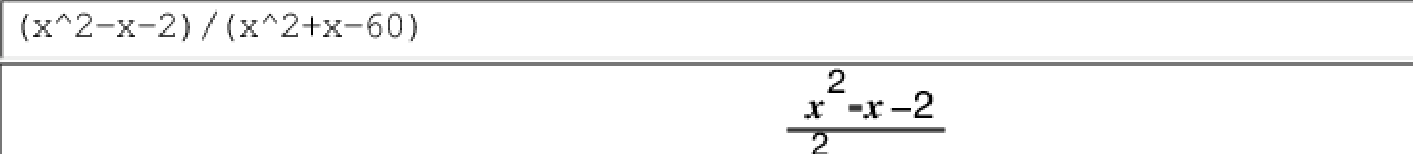
\includegraphics[width=\textwidth]{factoriser}\end{center}

Puis on met en surbrillance $x^2-x-2$ et on clique sur {\tt factoriser} du menu 
{\tt Reecriture} ou sur  {\tt factoriser} du clavier {\tt kbd} et on obtient :
\begin{center}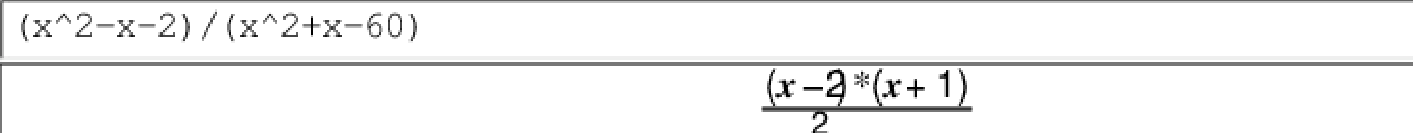
\includegraphics[width=\textwidth]{factorise}\end{center}

{\bf Exercices}\\
Factoriser :
\begin{enumerate}
\item $(a+b)^3+(a+b)^2$
\item $a^2+4ab+4b^2-1$
\item $4a^2-4a-4b^2+1$
\item $(4a-1)^2*+(8a+2)(a+5)$
\item $(3a-5)(a+6)+(5-3a)(a-3)+9a-15)$
\item $bc(b-c)+ca(c-a)+ab(a-b)$
\end{enumerate}
{\bf Solutions} avec {\tt Xcas}
\begin{enumerate}
\item On tape :\\
{\tt factoriser((a+b)\verb|^|3+(a+b)\verb|^|2)}\\
On obtient :\\
{\tt (a+b)\verb|^|2*(a+b+1)}
\item On tape :\\
{\tt factoriser(a\verb|^|2+4a*b+4b\verb|^|2-1)}\\
On obtient :\\
{\tt (a+2*b-1)*(a+2*b+1)}
\item On tape :\\
{\tt factoriser(4a\verb|^|2-4a-4b\verb|^|2+1)}\\
On obtient :\\
{\tt (2*a-2*b-1)*(2*a+2*b-1)}
\item On tape :\\
{\tt factoriser((4a-1)\verb|^|2*+(8a+2)*(a+5))}\\
On obtient :\\
{\tt 2*(a+5)*(4*a-1)\verb|^|2*(4*a+1)}
\item On tape :\\
{\tt factoriser((3a-5)*(a+6)+(5-3a)*(a-3)+9a-15))}\\
On obtient :\\
{\tt 12*(3*a-5)}
\item On tape :\\
{\tt factoriser(b*c*(b-c)+c*a*(c-a)+a*b*(a-b))}\\
On obtient :\\
{\tt (c-a)*(b-a)*(b-c)}
\end{enumerate}
\chapter{Arithm\'etique}
\section{La division euclidienne dans $\N$}\index{iquorem}\index{iquo}\index{irem}
Soient $a \in \N$ et $b\in \N$.\\
On \'ecrit $a=b*q+r$ avec $q \in \N$ et $r\in \N$ qui v\'erifie $0\leq r<b$.\\
On dit que $q$ est le quotient de la division euclidienne de $a$ par $b$ et que $r$ est le reste de la division euclidienne de $a$ par $b$.\\
On a :
$0\leq a-b*q<b$\\
On peut trouver $q$ et $r$ avec des soustractions successives.\\
On tape :
\begin{verbatim}
quoreste(a,b):={
local q;
q:=0;
tantque a>=b faire 
a:=a-b;
q:=q+1;
ftantque
retourne [q,a];
}:;
\end{verbatim}
Dans {\tt Xcas} cette fonction existe d\'ej\`a et s'appelle {\tt iquorem}.\\
On tape :\\
{\tt iquorem(45,7)}\\
On obtient :\\
{\tt [6,3]}\\
En effet $45=6*7+3$\\
Il existe aussi {\tt iquo(a,b)} qui renvoie le quotient {\tt q} de la division 
euclidienne de $a$ par $b$ et {\tt irem(a,b)} qui renvoie le reste {\tt r} de 
la division euclidienne de $a$ par $b$.\\
On tape :\\
{\tt iquo(45,7)}\\
On obtient : {\tt 6}\\
On tape :\\
{\tt irem(45,7)}\\
On obtient : {\tt 3}\\
Si $r$={\tt irem}$(a,b)$ est nul, on dit que $a$ est un multiple de $b$ et que 
$b$ est un diviseur de $a$.

\section{Le PGCD}\index{tantque}\index{faire}\index{ftantque}\index{retourne}
Le $PGCD(a,b)$ est le plus grand commun diviseur de $a$ et de $b$.\\
Pour calculer le $PGCD(a,b)$ on utilise l'algorithme d'Euclide qui utilise le 
fait que :
si $r$ est le reste de la division euclidienne de $a$ par $b$ alors :\\
$PGCD(a,b)=PGCD(b,r)$.\\
En effet si $a=bq+r$ tous les diviseurs communs \`a $a$ et $b$ sont aussi des 
diviseurs de $r$ et tous les diviseurs communs \`a $b$ et $r$ sont aussi des 
diviseurs de $a$.\\
Donc on cherche le $PGCD(b,r)$ et $r<b$ et on recommence. \`A chaque \'etape 
les restes sont positifs ou nuls et strictement d\'ecroissants donc il va 
arriver un moment ou un reste sera nul et donc le $PGCD(a,b)$ sera \'egal au 
dernier reste non nul.\\
On tape en utilisant :\\
{\tt tantque <condition> faire <instructions> ftantque} qui teste la condition
si <condition> est vraie les <instructions> sont ex\'ecut\'es puis on teste  
<condition> ...et on s'arr\^ete quand <condition> devient fausse.\\
{\tt retourne} renvoie la valeur de la fonction (ici renvoie le PGCD(a,b)).
\begin{verbatim}
PGCD(a,b):={
local r;
tantque b>0 faire 
r:=irem(a,b);
a:=b
b:=r;
ftantque
retourne a;
}:;
\end{verbatim}
On tape :\\
{\tt PGCD(45,30)}\\
On obtient :\\
{\tt 15}\\
On tape :\\
{\tt PGCD(30,45)}\\
On obtient :\\
{\tt 15}\\
On tape :\\
{\tt PGCD(45,30)}\\
On obtient :\\
{\tt 15}\\
On tape :\\
{\tt PGCD(1234567890,12345678)}\\
On obtient :\\
{\tt 18}\\
{\bf Remarque}\\
Lorsque $a<b$ on a $a=0*b+a$ donc le premier reste trouv\'e est $a$. On cherche 
ensuite le reste de  $b$ par $a$...dans l'exemple {\tt PGCD(30,45)}
l'algorithme dit :\\
le reste de 30 par 45 est 30\\
le  reste de 45 par 30 est 15\\
le  reste de 30 par 15 est 0\\
le premier reste non nul est donc 15 donc :\\
{\tt PGCD(45,30)=15} \\
Dans {\tt Xcas} cette fonction existe d\'eja et s'appelle {\tt gcd}.
On tape {\tt gcd(45,30)} et on obtient {\tt 15}\\
{\bf Exercice}\index{idivis}\index{gcd}
Un terrain rectangulaire a comme dimension 60 m de long et 45 m de large.\\
On veut planter des arbres r\'eguli\`erement espac\'es tout autour du terrain.
Quelle doit \^etre la distance entre 2 arbres consecutifs si on veut qu'il y 
ait un arbre sur chaque sommet du rectangle et si on veut que cette distance 
soit un nombre entier de m\`etres ?
{\bf Solution avec {\tt Xcas}}
{\tt idivis} renvoie la liste de tous les diviseurs d'un nombre entier.\\
{\tt gcd} renvoie le PGCD de 2 nombres entiers\\
La distance cherch\'ee est un diviseur commun \`a 60 et 45.\\
On tape :\\
{\tt gcd(60,45)}\\
On obtient : {\tt 15}\\
On tape pour avoir tous les diviseurs de 15 :\\
{\tt idivis(15)}\\
On obtient : {\tt [1,3,5,15]}\\
Donc la distance entre 2 arbres pourra \^etre 1m, 3m, 5m ou 15m.

\section{Rendre une fraction irr\'eductible}
Pour rendre une fraction $N/D$ ($N\in \Z$ et $D\in \Z$) irr\'eductible il faut 
diviser son num\'erateur $N$ et son d\'enominateur $D$ par le PGCD($N,D$).\\
{\tt Xcas} simplifie automatiquement une fraction en une fraction 
irr\'eductible.\\
On tape :\\
{\tt 12345678/3429355}\\
On obtient : {\tt 18/5}\\
On tape :\\
{\tt gcd(12345678,3429355)}\\
On obtient : {\tt 685871}\\
On tape :\\
{\tt 12345678/685871,3429355/685871}\\
On obtient : {\tt 18,5}

\chapter{\'Equations et in\'equations}
\section{R\'esoudre $x^2=a$}
Si $a<0$ il n'y a pas de solution\\
Si $a=0$ il y a  1 solution qui est $x=0$\\
Si $a>0$ il y a  2 solutions qui sont $x=-\sqrt a$ ou $x=\sqrt a$\\
Avec {\tt Xcas}\\
On tape :\\
{\tt resoudre(x\verb|^|2=-2)}\\
On obtient : {\tt []}\\
On tape :\\
{\tt resoudre(x\verb|^|2=2)}\\
On obtient : {\tt [-sqrt(2),sqrt(2)]}\\
On tape :\\
{\tt resoudre(x\verb|^|2=4+2*sqrt(3))}\\
On obtient : {\tt [-(sqrt(3))-1,sqrt(3)+1]}
\section{R\'esoudre une \'equation produit}
On sait qu'un produit de facteurs est nul si et seulement si un des facteur 
est nul.
Si un \'equation est mise sous la forme d'un produit, elle est donc facilement r\'esoluble.\\
{\bf Exercices}
\begin{enumerate}
\item R\'esoudre les \'equations :
\begin{itemize}
\item[$\bullet$] $(6x-1)^2+(2x-4)^2=10x(4x-2)$
\item[$\bullet$] $(3x+2)^2+7(3x+2)+5(9x^2-4)=0$
\end{itemize}
\item R\'esoudre et discuter suivant les valeurs de $m$ les \'equations :
\begin{itemize}
\item[$\bullet$] $2mx-1=x+7$
\item[$\bullet$] $(m-1)x+2x-3=m-1$
\end{itemize}
\end{enumerate}
{\bf Les solutions avec {\tt Xcas}}
\begin{enumerate}
\item R\'esoudre les \'equations :
\begin{itemize}
\item[$\bullet$] $(6x-1)^2+2x-4)^2=10x(4x-2)$\\
On tape:\\
{\tt resoudre((6x-1)\verb|^|2+(2x-4)\verb|^|2=10x*(4x-2))}\\
On obtient : {\tt [17/8]}\\
Pour avoir le d\'etail des calculs, on tape :\\
{\tt developper((6x-1)\verb|^|2+(2x-4)\verb|^|2=10x*(4x-2))}\\
On obtient : {\tt 40*x\verb|^|2-28*x+17=(40*x\verb|^|2-20*x)}\\
Donc $8x=17$ i.e. $x=17/8$
\item[$\bullet$] $(3x+2)^2+7(3x+2)+5(9x^2-4)=0$\\
On tape:\\
{\tt resoudre((3x+2)\verb|^|2+7*(3x+2)+5*(9x\verb|^|2-4)=0)}\\
On obtient : {\tt [-2/3,1/18]}\\
Pour avoir le d\'etail des calculs, on tape :\\
{\tt factoriser((3x+2)\verb|^|2+7*(3x+2)+5*(9x\verb|^|2-4))}\\
On obtient : {\tt (3*x+2)*(18*x-1)}\\
Donc $(3x+2)(18x-1)=0$ si et seulement si $3x+2=0$ ou si $18x-1=0$ i.e.
$x=-2/3$ ou $x=1/18$
\end{itemize}
\item R\'esoudre et discuter suivant les valeurs de $m$ les \'equations :
\begin{itemize}
\item[$\bullet$] $2mx-1=x+7$\\
On tape:\\
{\tt resoudre(2*m*x-1=x+7)}\\
On obtient : {\tt [8/(2*m-1)]}\\
{\bf Attention} \\
{\tt Xcas} ne renvoie que le cas g\'en\'eral qui n'est valable 
ici que si $m\neq 1/2$.
\item[$\bullet$] $(m-1)x+2x-3=m-1$\\
On tape:\\
{\tt resoudre((m-1)*x+2x-3=m-1)}\\
On obtient : {\tt [(m+2)/(m+1)]}\\
{\bf Attention} \\
{\tt Xcas} ne renvoie que le cas g\'en\'eral qui n'est valable ici que si 
$m\neq -1$
\end{itemize}
\end{enumerate}


\section{R\'esoudre une in\'equation}
Dans une in\'equation on peut faire passer un terme d'un membre \`a l'autre \`a
condition de changer son signe.\\
Dans une in\'equation on peut diviser ou multiplier les 2 membres d'une 
in\'equation par un nombre strictement positif sans changer le sens de 
l'in\'equation et par un nombre strictement n\'egatif en changeant le sens de 
l'in\'equation.\\
{\bf Exercices}
\begin{enumerate}
\item R\'esoudre les \'equations :
\begin{itemize}
\item[$\bullet$] $(6x-1)^2+(2x-4)^2=10x(4x-2)$
\item[$\bullet$] $(3x+2)^2+7(3x+2)+5(9x^2-4)=0$
\end{itemize}\item R\'esoudre les in\'equations :
\begin{itemize}
\item[$\bullet$] $3(x-1)+7(3x-2)<6(x+1)$
\item[$\bullet$] $\displaystyle \frac{3x-4}{x-1}>=3$
\end{itemize}
\item R\'esoudre et discuter suivant les valeurs de $m$ les in\'equations :
\begin{itemize}
\item[$\bullet$] $m(x-3)>x+2$
\item[$\bullet$] $m(x-1)+(x-3)(x-7)>(x+1)^2$
\end{itemize}
\end{enumerate}
{\bf Les solutions avec {\tt Xcas}}
\begin{enumerate}
\item R\'esoudre les in\'equations :
\begin{itemize}
\item[$\bullet$] $3(x-1)+7(3x-2)<6(x+1)$\\
On tape :\\
{\tt  resoudre(3*(x-1)+7*(3x-2)<6*(x+1))}\\
On obtient : {\tt [x<(23/18)]}\\
Pour avoir le d\'etail des calculs, on tape :\\
{\tt E:=(3*(x-1)+7*(3x-2)<6*(x+1))}\\
On obtient : {\tt (6*(x+1))>(3*(x-1)+7*(3*x-2))}\\ 
{\bf Attention}\\
{\tt Xcas} \'ecrit toujours une in\'equation avec le signe {\tt >} ou {\tt >=}.\\
On tape :\\
{\tt developper(gauche(E)-droit(E))}\\
On obtient : {\tt -18*x+23}\\
$-18*x+23>0$ est \'equivalent \`a $23>18x$ donc $x<\frac{23}{18}$
\item[$\bullet$] $\displaystyle \frac{3x-4}{x-1}>=3$\\
On tape :\\
{\tt resoudre((3*x-4)/(x-1)>=3)}\\
On obtient : {\tt [x<1]}\\
Pour avoir le d\'etail des calculs, on tape :\\
{\tt E:=(3*x-4)/(x-1)>=3}\\
{\tt factoriser(gauche(E)-droit(E))}\\
On obtient : {\tt -1/(x-1)}\\
$-1/(x-1)>=0$ est \'equivalent \`a $x-1<0$ donc \`a $x<1$
\end{itemize}
\item R\'esoudre et discuter suivant les valeurs de $m$ les in\'equations :
\begin{itemize}
\item[$\bullet$] $m(x-3)>x+2$\\
On tape :\\
{\tt purge(m);resoudre(m*(x-3)>x+2,x)} 
On obtient :\\
{\tt  un message donnant la solution de l'\'equation correspondante ici 
$(3m+2)/(m-1)$}\\
On tape :\\
{\tt supposons(m>1);}\\
{\tt resoudre(m*(x-3)>x+2,x)}\\
On obtient : {\tt [x>((3*m+2)/(m-1))]}\\
On tape :\\
{\tt supposons(m<1);}\\
{\tt resoudre(m*(x-3)>x+2,x)}\\
On obtient : {\tt [x<((3*m+2)/(m-1))]}\\
Pour avoir le d\'etail des calculs, on tape :\\
{\tt E:=m*(x-3)>x+2}\\
{\tt developper(gauche(E)-droit(E))}\\
On obtient : {\tt (m-1)*x-3*m-2}\\
Donc $(m-1)*x>3*m+2$ et on termine \`a la main :\\
si $m>1$ alors la solution est $\displaystyle x>\frac{3*m+2}{m-1}$\\
si $m<1$ alors la solution est $\displaystyle x<\frac{3*m+2}{m-1}$\\
si $m=1$  alors $3*m+2=5$ donc il n'y a pas de solution.

\item[$\bullet$] $m(x-1)+(x-3)(x-7)>(x+1)^2$\\
On tape :\\
{\tt purge(m);resoudre(m*(x-1)+(x-3)*(x-7)>(x+1)\verb|^|2,x)} renvoie un 
message donnant
la solution de l'\'equation correspondante ici $(m-20)/(m-12)$\\
On tape alors :\\
{\tt supposons(m>12)}\\
{\tt resoudre(m*(x-1)+(x-3)*(x-7)>(x+1)\verb|^|2,x)} renvoie un message donnant
On obtient : {\tt [x>((m-20)/(m-12))]}\\
On tape alors :\\
{\tt supposons(m<12)}\\
{\tt resoudre(m*(x-1)+(x-3)*(x-7)>(x+1)\verb|^|2,x)} renvoie un message donnant
On obtient : {\tt [x<((m-20)/(m-12))]}\\
Pour avoir le d\'etail des calculs, on tape :\\
{\tt E:=m*(x-1)+(x-3)*(x-7)>(x+1)\verb|^|2}\\
{\tt developper(gauche(E)-droit(E))}\\
On obtient : {\tt (m-12)*x-m+20}\\
Donc $(m-12)*x>m-20$ et on termine \`a la main :\\
si $m>12$ alors la solution est $\displaystyle x>\frac{m-20}{m-12}$\\
si $m<12$ alors la solution est $\displaystyle x<\frac{m-20}{m-12}$\\
si $m=12$  alors $m-20=-8$ donc l'in\'equation est verifi\'ee pour tout 
$x \in \R$.
\end{itemize}
\end{enumerate}
\section{R\'esoudre une \'equation ou une in\'equation graphiquement}\index{plotfunc}\index{in}\index{inter}\index{droite}\index{abscisse}\index{affichage}
Il peut \^etre interressant de visualiser la ou les solutions d'une \'equation 
ou d'une in\'equation en la rep\'esentant graphiquement.\\
Reprenons les exemples pr\'ec\'edents :
\begin{enumerate}
\item R\'esoudre les \'equations :
\begin{itemize}
\item[$\bullet$] $(6x-1)^2+(2x-4)^2=10x(4x-2)$
\item[$\bullet$] $(3x+2)^2+7(3x+2)+5(9x^2-4)=0$
\end{itemize}
\item R\'esoudre les in\'equations :
\begin{itemize}
\item[$\bullet$] $3(x-1)+7(3x-2)<6(x+1)$
\item[$\bullet$] $\displaystyle \frac{3x-4}{x-1}>=3$
\end{itemize}
\end{enumerate}
{\bf Les solutions graphiques avec {\tt Xcas}}
\begin{enumerate}
\item R\'esoudre les \'equations :
\begin{itemize}
\item[$\bullet$] $(6x-1)^2+(2x-4)^2=10x(4x-2)$
On tape :\\
{\tt G1:=plotfunc((6x-1)\verb|^|2+(2x-4)\verb|^|2-10x*(4x-2))}\\
On obtient apr\`es avoir fait un grossissement (cliquez sur {\tt in} et sur {\tt auto}) :\\
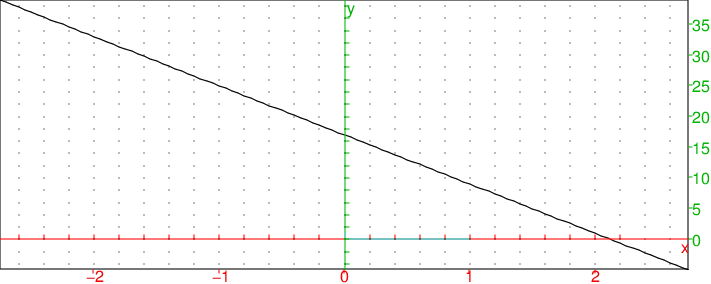
\includegraphics[width=\textwidth]{equagraph1}\\
On tape :\\
{\tt abscisse(inter(G1,droite(y=0)))}\\
On obtient :
{\tt [17/8]}
\item[$\bullet$] $(3x+2)^2+7(3x+2)+5(9x^2-4)=0$
On tape :\\
{\tt G2:=plotfunc((3x+2)\verb|^|2+7*(3x+2)+5*(9x\verb|^|2-4))}\\
puis apr\`es avoir vu que la courbe coupe l'axe des $x$ entre-1 et 1, on tape :\\
{\tt plotfunc((3x+2)\verb|^|2+7*(3x+2)+5*(9x\verb|^|2-4),x=-1..1)}\\
On obtient apr\`es avoir fait un grossissement (cliquez sur {\tt in} et sur {\tt auto}) :\\
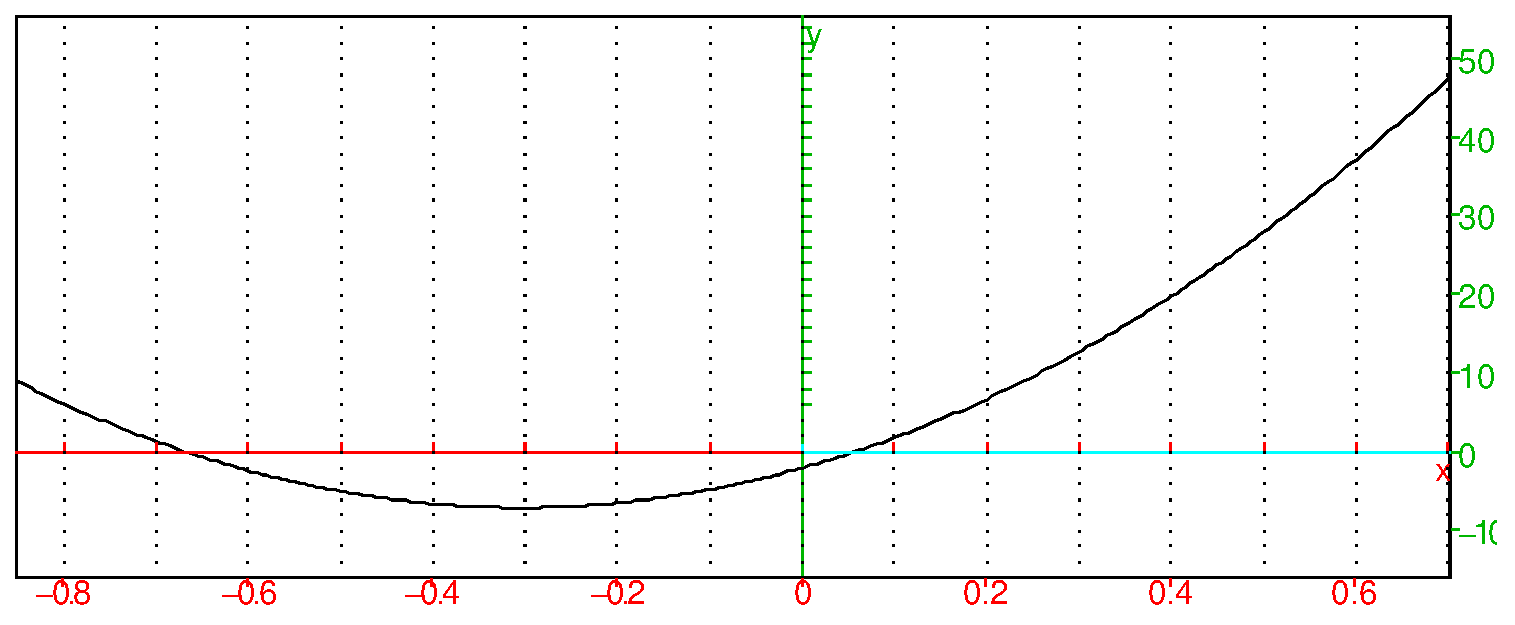
\includegraphics[width=\textwidth]{equagraph2}\\
On tape :\\
{\tt abscisse(inter(G2,droite(y=0)))}\\
On obtient :
{\tt [-2/3,1/18]}
\end{itemize}
\item R\'esoudre les in\'equations :
\begin{itemize}
\item[$\bullet$] $3(x-1)+7(3x-2)<6(x+1)$
On tape :\\
{\tt d1:=droite(y=3*(x-1)+7*(3x-2),affichage=rouge);}\\
{\tt d2:=droite(y=-6*(x+1),affichage=bleu)}\\
On obtient :\\
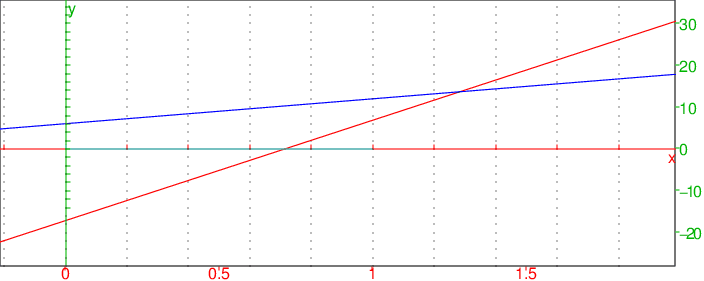
\includegraphics[width=\textwidth]{equagraph3}\\
On tape :\\
{\tt abscisse(inter(d1,d2))}\\
On obtient :
{\tt [23/18]}\\
Les points de la droite bleue sont au dessus des points de la droite rouge lorsque $x>23/18$.
\item[$\bullet$] $\displaystyle \frac{3x-4}{x-1}>=3$
On tape :\\
{\tt plotfunc((3x-4)/(x-1),x,affichage=rouge),droite(y=3,affichage=bleu),\\ droite(x=1,affichage=vert)}\\
On obtient :\\
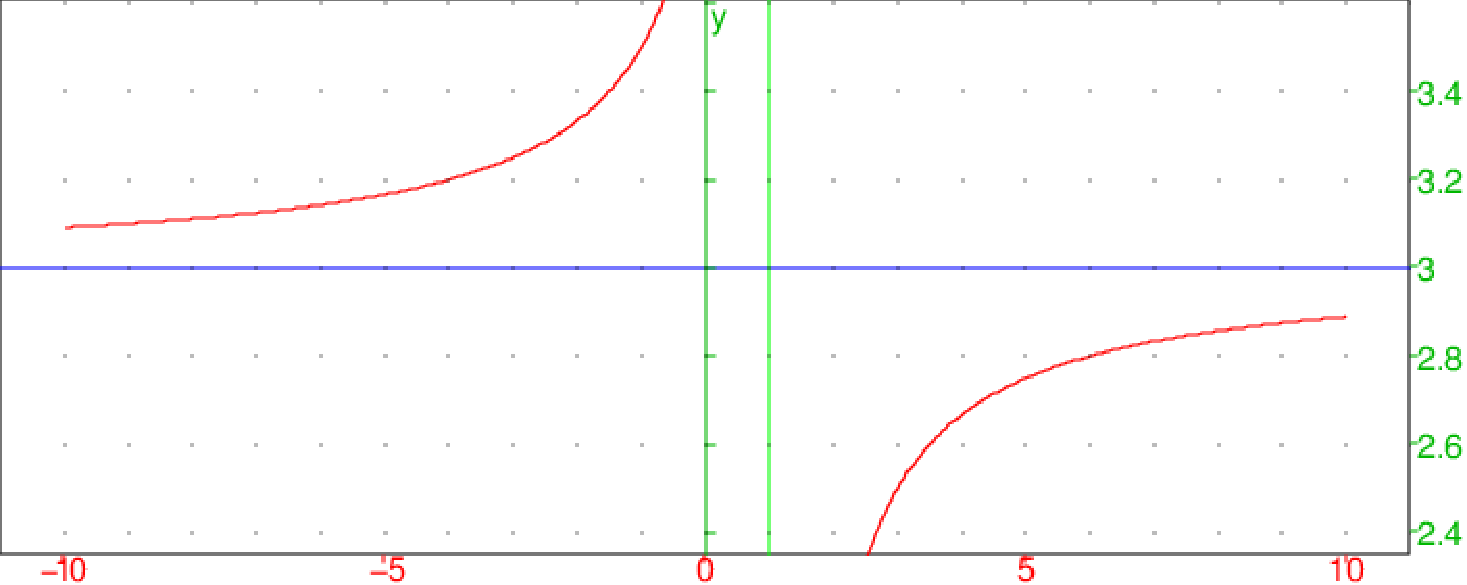
\includegraphics[width=\textwidth]{equagraph4}\\
Les points de la la courbe rouge sont au dessus des points de la droite bleue lorsque $x<1$.
\end{itemize}
\end{enumerate}


\chapter{Syst\`emes d'\'equations}
\section{R\'esoudre un syst\`eme par substitution}\index{resoudre\_systeme\_lineaire}\index{linsolve}
Soit le syst\`eme :\\
$$\left\{
\begin{array}{l}
2x-5y=8\\
3x+4y=2
\end{array}
\right.
$$
La 1-i\`ere \'equation donne :\\
$\displaystyle y=\frac{2x-8}{5}$\\
Donc le syst\`eme est \'equivalent \`a :
$\left\{
\begin{array}{lrl}
 &y&=\displaystyle\frac{2x-8}{5}\\
3x+&4y&=2
\end{array}
\right.
$\\
En substituant $y$ dans la deuxi\`eme \'equation, le syst\`eme est 
\'equivalent \`a :\\
$\left\{
\begin{array}{lrl}
 &y&=\displaystyle\frac{2x-8}{5}\\
3x+&4\displaystyle\frac{2x-8}{5}&=2
\end{array}
\right.
$\\
La 2-i\`eme \'equation donne :\\
$15x+8x-32=10$ \\
$23x=42$\\
$\displaystyle x=\frac{42}{23}$\\
En reportant cette valeur dans la 1-i\`ere \'equation on obtient :\\
$\displaystyle y=\frac{2\frac{42}{23}-8}{5}$\\
$\displaystyle y=\frac{84-8*23}{23*5}=-\frac{4*25}{23*5}-\frac{20}{23}$\\
Le syst\`eme :\\
$\left\{
\begin{array}{l}
2x-5y=8\\
3x+4y=2
\end{array}
\right.
$ admet donc comme solution :
$\displaystyle x=\frac{42}{23},y=-\frac{20}{23}$

Avec {\tt Xcas}, on tape :\\
{\tt linsolve([2x-5y=8,3x+4y=2],[x,y])}\\
ou bien\\
{\tt resoudre\_systeme\_lineaire([2x-5y=8,3x+4y=2],[x,y])}\\
On obtient :\\
{\tt [42/23,-20/23]}\\
\section{R\'esoudre un syst\`eme par combinaison}
La m\'ethode par combinaison consiste \`a \'eliminer une variable en remplacant
une \'equation par une combinaison lin\'eaire des 2 \'equations. Par exemple, 
on \'elimine $x$ dans la 2-i\`eme \'equation en faisant une combinaison des 
2 \'equations ce qui donne une nouvelle 2-i\`eme \'equation : le syst\`eme est 
alors \'equivalent au syst\`eme compos\'e de la 1-i\`ere \'equation et cette
nouvelle \'equation.\\
Soit le syst\`eme :\\
$$\left\{
\begin{array}{l}
2x-5y=8\\
3x+4y=2
\end{array}
\right.
$$
On remplace la deuxi\`eme \'equation par la combinaison :\\
3*1-i\`ere \'equation -2*2-i\`eme \'equation que l'on note:\\
$\left\{
\begin{array}{lr}
2x-5y=8 &\quad |*3\\
3x+4y=2 &\quad |*-2
\end{array}
\right.
$\\
Donc le syst\`eme est \'equivalent \`a :
$\left\{
\begin{array}{rrr}
2x&-5y=&8 \\
&-23y=&20
\end{array}
\right.
$\\
Donc $\displaystyle y=-\frac{20}{23}$\\
En reportant cette valeur dans la premi\`ere \'equation on obtient :\\
$\displaystyle 2x+5\frac{20}{23}=8$\\
$46x+5*20=8*23$\\
$46x=8*23-100=84$\\
$\displaystyle x=\frac{24}{23}$\\
Le syst\`eme :\\
$\left\{
\begin{array}{l}
2x-5y=8\\
3x+4y=2
\end{array}
\right.
$ admet donc comme solution :
$\displaystyle x=\frac{42}{23},y=-\frac{20}{30}$
\section{R\'esoudre un syst\`eme graphiquement}\index{inter\_droite}\index{point}\index{droite}\index{coordonnees}\index{equation}
R\'esoudre graphiquement le syst\`eme :\\
$$\left\{
\begin{array}{l}
2x-5y=8\\
3x+4y=2
\end{array}
\right.
$$
Chacune de ces \'equations prises s\'eparement est l'\'equation d'une droite et admet une infinit\'e de solutions qui sont les coordonn\'ees des points 
situ\'es sur cette droite.\\
Ce syst\`eme a donc comme solution les coordonn\'ees du point d'intersection
des droites d'\'equation :\\ 
$2x-5y=8$ et $3x+4y=2$
Tra\c{c}ons ces 2 droites :\\
La droite d'\'equation $2x-5y=8$ passe par les points :\\
$A$  de coordonn\'ees $x=4,y=0$ et $B$  de coordonn\'ees $x=-1,y=-2$\\
La droite d'\'equation $3x+4y=2$ passe par les points  :\\
$C$ de coordonn\'ees $x=0,y=1/2$ et $D$  de coordonn\'ees $x=2,y=-1$\\
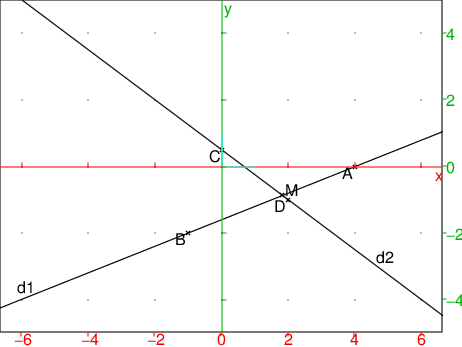
\includegraphics[width=\textwidth]{systgraph}\\
Avec {\tt Xcas}, on tape dans un niveau de g\'eom\'etrie $2d$:\\
{\tt d1:=droite(2x-5y=8)}\\
{\tt d2:=droite(3x+4y=2)}\\
On peut placer les points $A,B,C,D$ en tapant :\\
{\tt A:=point(4)}\\
{\tt B:=point(-1,-2)}\\
{\tt C:=point(0,1/2)}\\
{\tt D:=point(2,-1)}\\
Le point d'intersection de $d_1$ et $d_2$ est obtenu en tapant :\\
{\tt M:=inter\_droite(d1,d2)}\\
{\tt coordonnees(M)}\\
On obtient :\\
{\tt [42/23,-20/23]}\\
On remarquera qu'en faisant juste le dessin sur une feuille de papier, on ne 
pourra pas en g\'en\'eral, d\'eterminer les valeurs exactes des coordonn\'ees 
du point d'intersection mais seulement leurs valeurs approch\'ees.\\
{\bf Exercice}\\
Dans un rep\`ere orthonorm\'e $(O,x,y)$ repr\'esenter graphiquement les 
droites $d_1$ et $d_2$ qui ont comme \'equation respective 
$2x+y=5$ et $2x-y=3$\\
Soit $A$ le point d'intersection de $d_1$ et $d_2$.\\
 D\'eterminer graphiquement les coordonn\'ees de $A$ point d'intersection 
et v\'erifier le r\'esultat obtenu\\
 D\'eterminer l'\'equation de la droite $OA$.\\
{\bf Solution avec {\tt Xcas}}\\
On tape dans un niveau de g\'eom\'etrie $2d$ :\\
{\tt O:=point(0);}
{\tt d1:=droite(2x+y=5);}\\
{\tt d2:=droite(2x-y=3);}\\
{\tt A:=inter\_droite(d1,d2)}\\
{\tt d:=droite(0,A,affichage=4);}\\
On obtient : \\
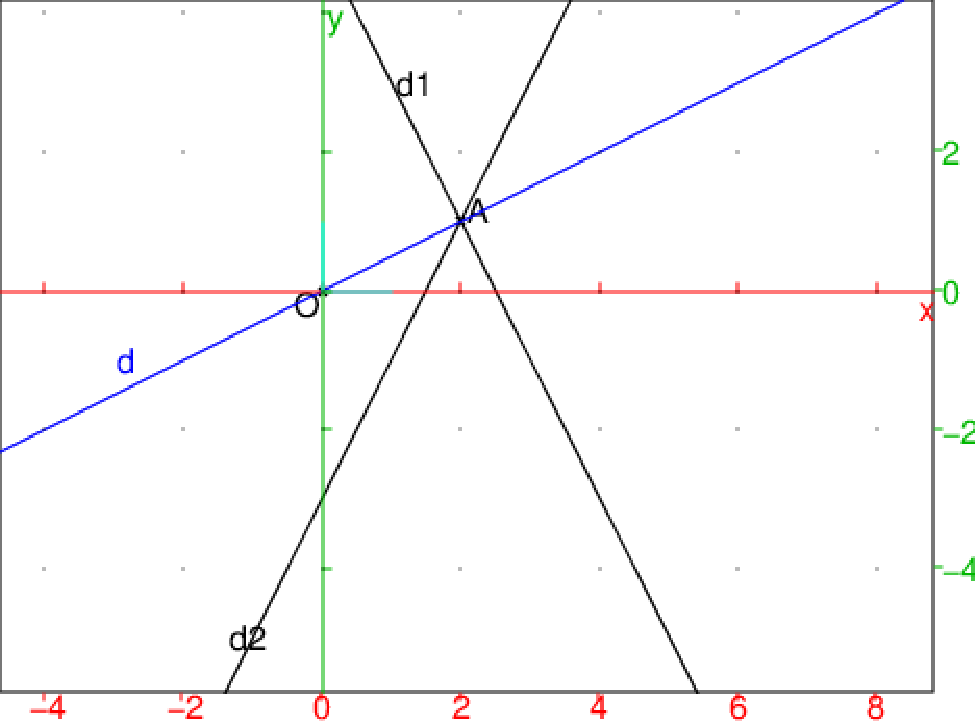
\includegraphics[width=\textwidth]{systgraph2}\\
On tape :\\
{\tt coordonnees(A);}\\
On obtient : {\tt [2,1]}\\
et on v\'erifie que l'on a bien :\\
$2*2+1=5$ et $2*2-1=3$\\
On tape :\\
{\tt equation(d);}\\
On obtient : {\tt y=x/2}\\
On remarque que la somme des 2 
\'equations \'elimine $y$. On va donc remplacer la 2-i\`eme \'equation par la 
somme des 2 \'equations et le syst\`eme est \'equivalent \`a :\\
$2x+y=5$ et $4x=8$ \'equivalent \`a\\
$x=2$ et $4+y=5$ \'equivalent \`a\\
$x=2$ et $y=1$ \\
On tape avec {\tt Xcas} :\\
{\tt resoudre\_systeme\_lineaire([2x+y=5,4+y=5],[x,y])}\\
On obtient : {\tt [2,1]}
\section{Exercices se ramenant \`a la r\'esolution d'un syst\`eme}\index{abcuv}
\index{legende}\index{evalf}\index{quadrant3}
\begin{enumerate}
\item
On paye une somme de 100 euros avec des $x$ pi\`eces de 2 euros et $y$  billets
 de 5 euros. Le nombre de pi\`eces et de billet est 26.
Calculer le nombre de pi\`eces et le nombre de billets. On donnera une solution
\`a l'aide d'une m\'ethode graphique, d'une m\'ethode alg\'ebrique et d'une 
m\'ethode arithm\'etique.\\
Le probl\`eme est-il possible si le nombre de pi\`eces et le nombre de billets
est un nombre entier $m$ quelconque.\\

{\bf M\'ethode graphique} avec {\tt Xcas}\\
On tape :\\
{\tt d1:=droite(x+y=26,affichage=bleu)}\\
{\tt d2:=droite(2x+5y=100):;affichage(d2,vert)}\\
{\tt legende(20*i,"d2",quadrant3,vert)}\\
{\tt A:=inter\_droite(d1,d2)}\\
On obtient :\\
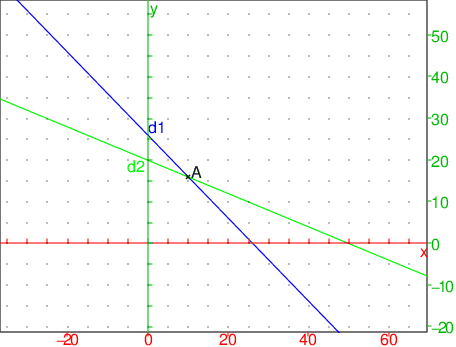
\includegraphics[width=\textwidth]{systgraph1}\\
On tape :\\
{\tt coordonnees(A)}\\
On obtient :\\
{\tt [10,16]}\\
Donc il y a 10 pi\`eces de 2 euros et 16 billets de 5 euros.\\
{\bf M\'ethode alg\'ebrique} avec {\tt Xcas}\\
On tape :\\
{\tt linsolve([x+y=26,2x+5y=100],[x,y])}\\
On obtient :\\
{\tt [10,16]}\\
Donc il y a 10 pi\`eces de 2 euros et 16 billets de 5 euros.\\
{\bf M\'ethode arithm\'etique}\\ 
On cherche $x \in \N$ et $y \in \N$ tel que :\\
$x+y=26$ et $2x+5y=100$\\
Pour r\'esoudre $2x+5y=100$ avec des entiers relatifs on cherche une solution 
particuli\`ere de $2x+5y=100$ et on ajoute la solution g\'en\'erale de 
$2x+5y=0$ qui est $x=-5k,y=2k$.\\
Pour avoir une  solution particuli\`ere de $2x+5y=100$, avec des entiers de 
$\Z$, avec {\tt Xcas}, on tape :\\
{\tt abcuv(2,5,100)}\\
On obtient :\\
{\tt [50,0]}\\
Donc $x=50-5k,y=2k$.\\
On veut que $x+y=26$ donc $50-3k=26$ soit $k=8$ donc :\\
$x=50-5*8=40$ et $y=2*8=16$\\ 
{\bf Syst\`eme  $x+y=m$ et $2x+5y=100$}\\
On a $20\leq m\leq 50$ car :\\
20 est la valeur minimum de $m$ qui correspond au nombre de billets de 5 euros 
 qu'il faut pour  payer 100 euros \\
50 est la valeur maximum de $m$ qui correspond au nombre de pi\`eces de 2 euros 
qu'il faut  pour  payer 100 euros\\
{\bf M\'ethode graphique} avec {\tt Xcas}, on tape :\\
{\tt assume(m=[0,20,50,1])}
{\tt d1:=droite(x+y=m,affichage=bleu)}\\
{\tt d2:=droite(2x+5y=100):;affichage(d2,vert)}\\
{\tt legende(20*i,"d2",quadrant3,vert)}\\
{\tt A:=inter\_droite(d1,d2)}\\
{\tt evalf(coordonnees(A))}\\
Il y a alors un curseur $m$ qui va de 1 en 1 de 20 jusque 50.\\
On peut suivre les valeur de la derni\`ere commande est voir que pour \\
$m=23$ les coordonn\'ees de $A$ sont (5,18),\\
$m=26$ les coordonn\'ees de $A$ sont (5,16),\\
$m=29$ les coordonn\'ees de $A$ sont (15,14), etc..\\
On peut donc conjecturer que $20-m$ doit \^etre un multiple de 3.\\
{\bf M\'ethode alg\'ebrique}\\
Avec {\tt Xcas}, on tape :\\
{\tt linsolve([x+y=m,2x+5y=100],[x,y])}\\
On obtient :\\
{\tt [5/3*m-100/3,-2/3*m+100/3]}\\
On tape :\\
{\tt factoriser([5/3*m-100/3,-2/3*m+100/3])}\\
On obtient :\\
{\tt [5*(m-20)/3,-2*(m-50)/3]}\\
les nombres $x$ et $y$ doivent \^etre des entiers naturels donc $m$ doit 
satisfaire aux conditions :\\
$m-20\geq 0$, $50-m\leq 0$ et\\
 $m-20$ et $m-50$ doivent \^etr e des multiples de 3.\\ 
Donc $20 \leq m \leq 50$, et $m=20+3*k=50-3*p$ ($k\in  \N$ et $p \in \N$\\
soit  $3(k+p)=30$ soit $k+p=10$ ce qui fait que l'on doit avoir :\\
$m=20+3k$ pour $k=0..10$.\\
Avec {\tt Xcas}, on tape :\\
{\tt M:=(20+3k)\$(k=0..10)}\\
On obtient les valeurs de $m$ possibles :\\
{\tt 20,23,26,29,32,35,38,41,44,47,50}\\
On tape :\\
{\tt SM:=([5*(M[k]-20)/3,-2*(M[k]-50)/3,20+3k]\$(k=0..10)}\\
On obtient les solutions $SM[k]$ et les valeurs de $m=M[k]$ correspondantes :\\
{\tt [0,20,20],[5,18,23],[10,16,26],[15,14,29],[20,12,32], [25,10,35],
[30,8,38],[35,6,41],[40,4,44],[45,2,47],}\\ 
{\tt [50,0,50][0,20],[5,18],[10,16],[15,14],[20,12],}\\
{\tt [25,10],[30,8],[35,6],[40,4],[45,2],[50,0]}\\
{\bf M\'ethode arithm\'etique}\\ 
Si $2x+5y=100$ avec $x \in \N$ et $y\in \N$ c'est que :\\
$x$ est divisible par 5 puisque $2x=100-5y=5(20-y)$  donc $x=5k$\\
$y$ est divisible par 2 puisque $5y=100-2x=2(50-x)$  donc $y=2p$\\
Le syst\`eme devient :\\
$x+y=5k+2p=m$ et $2x+5y=10k+10p=100$ soit \\
$5k+2p=m$ et $p=10-k$\\
$5k+20-2k=m$ et $p=10-k$\\
Donc $m=20+3k=50-3p$
\item Trouver les 2 facteurs d'un produit sachant que l'un est le triple de 
l'autre et que si on augmentait chacun de 4 le produit augmenterait de 224.\\
{\bf Solution}\\
Soient $x$ et $y$ les 2 facteurs on a :\\
$x=3y$ et $(x+4)(y+4)=xy+224$\\
Puisque $(x+4)(y+4)=xy+4(x+y+4)$, il faut r\'esoudre le syst\`eme :\\
$x=3y$ et $x+y=224/4-4=56-4=52$ ce qui revient \`a r\'esoudre le syst\`eme :\\
$x=3y$ et $3y+y=52$\\
Donc $y=13$ et $x=39$
V\'erifions :\\
$xy=13*39=507$ et $17*43=731$ et on a bien $731-507=224$\\
Avec {\tt Xcas}, on tape :\\
{\tt linsolve([x=3y,(x+4)*(y+4)=x*y+224],[x,y])}\\
On obtient :\\
{\tt [39,13]}
\item J'ai trois fois l'age de mon fils et quand mon fils aura l'age que j'ai
nous aurons ensemble 104 ans.\\
Quel est mon age et quel est celui de mon fils ?\\
{\bf Solution}\\
Soient $x$ mon age et $y$ celui de mon fils. On a :\\
$x=3y$ et mon fils aura l'age que j'ai dans $x-y$ ans
Dans $x-y$ ans j'aurai $x+x-y=2x-y$ ans et mon fils aura $x$ ans.
Ensemble on aura donc $2x-y+x=104$\\
Il faut donc r\'esoudre le syst\`eme :\\
$x=3y$ et $3x-y=104$ ce qui revient \`a r\'esoudre le syst\`eme :\\
$x=3y$ et $9y-y=8y=104$\\
Donc $y=104/8=13$ et $x=39$.\\
V\'erifions :\\
Dans $39-13=26$ ans, j'aurai $39+26=65$ ans et mon fils aura $13+26=39$ ans.
Ensemble on aura bien $65+39=104$ ans\\  
Avec {\tt Xcas}, on tape :\\
{\tt linsolve([x=3y,2x-y+x=104],[x,y])}\\
On obtient :\\
{\tt [39,13]}
\end{enumerate}
\chapter{Notion de fonction}\index{subst}\index{:=}
Il ne faut pas confondre expression et fonction.
Une expression est une combinaison de nombres et de variables
reli\'es par des op\'erations alors qu'une 
fonction associe \`a une variable une expression. Par exemple,
\verb|a:=x^2+2*x+1| définit une expression et
\verb|b(x):=x^2+2*x+1| définit une fonction. 
On obtient la valeur de l'expression \verb|a| en 0, avec
\verb|subst(a,x=0)| et  la valeur de la fonction \verb|b| en 0, 
avec \verb|b(0)|.
\section{Image d'un nombre par une fonction}\index{\$}
Soit $f$ est une fonction de $\R$ dans $\R$. Cela veut dire que pour tout 
$a$ dans $\R$ $f$ associe le nombre $f(a)$ de $\R$. On dit que  $f(a)$ estv l'image de $qa$ par $f$.\\
{\bf Exemple}\\
Soit $f(x)=x^3-3x+2$.
Trouver l'image des nombres -2,-1,0,1,2
Avec {\tt Xcas}, on tape :\\
{\tt f(x):=x\verb|^|3-3x+2}\\
{\tt f(k)\$(k=-2..2)}\\
On obtient les valeurs de $f(-1),f(0),f(1),f(2)$ :\\
{\tt 0,4,2,0,4}\\
Factoriser $f(x)$.\\
$f(x)$ s'annule pour $x=1$ et pour $x=-2$ donc $(x-1)$ et $(x+2)$ sont des 
facteurs de $f(x)$.\\
Donc $f(x)=(x-1)*(ax^2+bx+c)=x^3-3x+2$\\
On en d\'eduit par identification que $a=1$, $c=-2$ et $b-a=0$ donc  
$f(x)=(x-1)(x^2+x-2)$\\
$x^2+x-2$ s'annule lorsque $x=-2$ donc $x^2+x-2=(x+2)(x-1)$ d'o\`u 
$f(x)=(x-1)^2(x+2)$\\
Avec {\tt Xcas}, on tape :\\
{\tt factoriser(f(x))}\\
On obtient :\\
{\tt (x-1)\verb|^|2*(x+2)}

\section{Ant\'ec\'edent(s) d'un nombre par une fonction}\index{resoudre}
Les ou l'ant\'ec\'edent(s) d'un nombre $b$ par une fonction $f$ sont les 
nombres $a$ tels que $f(a)=b$.\\
{\bf Exemple}\\
Soit $f(x)=x^3-3x+2$.\\
Trouver les ant\'ec\'edent(s) des nombres 0,2,4.\\
Avec {\tt Xcas}, on tape :\\
{\tt solve(f(x)=0,x)}\\
On obtient :\\
{\tt [-2,1]}\\
On tape :\\
{\tt solve(f(x)=2,x)}\\
On obtient :\\
{\tt [-(sqrt(3)),0,sqrt(3)]}\\
On tape :\\
{\tt resoudre(f(x)=4,x)}\\
On obtient :\\
{\tt [-1,2]}
\section{Graphe d'une fonction}\index{plotfunc}
Le graphe d'une fonction est l'ensemble des points de coordonn\'ees 
$x,f(x)$ dans un rep\`ere $Oxy$

{\bf Exemple}\\
Soit $f(x)=x^3-3x+2$.\\
Tracer le graphe de $f$ sur l'intervalle [-3,3].\\
On tape :\\
{\tt plotfunc(f(x),x=-3..3))}\\
On obtient :\\
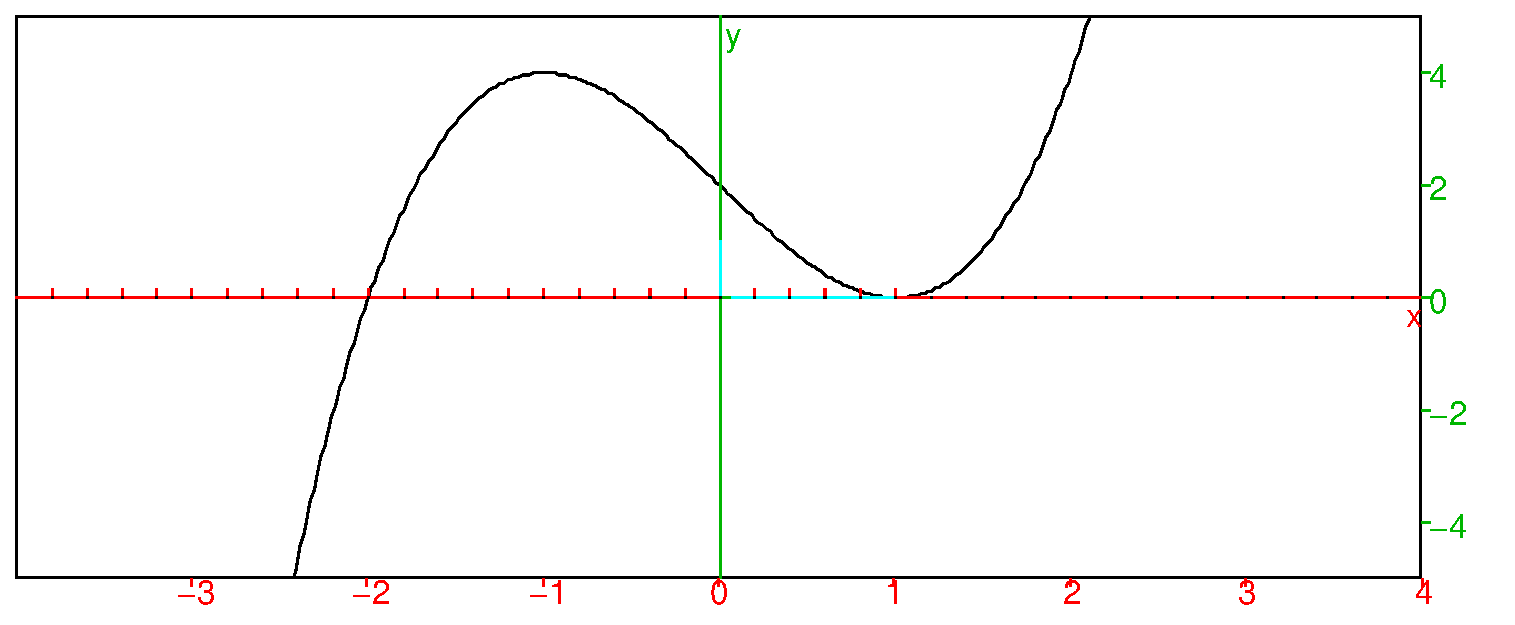
\includegraphics[width=\textwidth]{graphef}
\chapter{Fonctions lin\'eaires et affines}\index{droite}
Une fonction lin\'eaire r\'eelle est une fonction de la forme $f(x)=ax$ avec 
$x\in \R$ et $a\in \R$\\
Une fonction affine r\'eelle est une fonction de la forme $f(x)=ax+b$ avec 
$x\in \R$, $a\in \R$ et $b\in \R$ \\
\section{Repr\'esentation d'une fonction lin\'eaire}
Soit un rep\`ere orthonorm\'e $Oxy$.\\
La repr\'esentation graphique d'une fonction lin\'eaire $f(x)=ax$ est une 
droite passant par l'origine $O$ du rep\`ere et qui a comme de pente $a$.
On dit que cette droite a pour \'equation $y=ax$\\
Avec {\tt Xcas}, on ouvre un niveau de g\'eom\'etrie 2d (Alt+g).\\
On clique sur {\tt Edit} de ce niveau et on choisit {\tt Ajouter param\`etre}.\\
Une boite de dialogue pr\'eremplie s'ouvre : on valide avec {\tt OK} et on 
obtient au niveau 1 comme ligne de commande :\\
{\tt assume(a=[0,-5,5,0.1])}\\
cela provoque la mise en place d'un curseur (sous le pav\'e situ\'e \`a 
droite de l\'ecran graphique) qui permet de changer les valeurs de {\tt a}.\\
On tape :\\
{\tt droite(y=a*x)}\\
Puis on fait bouger le curseur.\\
On obtient : {\tt Le graphe de la droite d'\'equation $y=ax$ pour diff\'erentes valeurs de $a$}\\

\section{Repr\'esentation d'une fonction affine}
Soit un rep\`ere orthonorm\'e $Oxy$.\\
La repr\'esentation  graphique d'une fonction affine $f(x)=ax+b$ est une droite
de pente $a$ passant par le point $B$ de coordonn\`ees $0,b$
On dit que cette droite a pour \'equation $y=ax+b$\\
Avec {\tt Xcas}, on ouvre un niveau de g\'eom\'etrie 2d (Alt+g).\\
On clique sur {\tt Edit} de ce niveau et on choisit {\tt Ajouter param\`etre}.\\
Une boite de dialogue pr\'eremplie s'ouvre : on valide avec {\tt OK} et on 
obtient au niveau 1 comme ligne de commande :\\
{\tt assume(a=[0,-5,5,0.1])}\\
cela provoque la mise en place d'un curseur (sous le pav\'e situ\'e \`a 
droite de l\'ecran graphique) qui permet de changer les valeurs de {\tt a}.\\
On refait la m\^eme chose ou on recopie la commande pour avoir au niveau 2
{\tt assume(b=[0,-5,5,0.1])}\\
cela provoque la mise en place d'un curseur (sous le pav\'e situ\'e \`a 
droite de l\'ecran graphique) qui permet de changer les valeurs de {\tt b}.\\
On tape :\\
{\tt droite(y=a*x+b)}\\
Puis on fait bouger le curseur {\tt a} et le curseur {\tt b}
On obtient : {\tt Le graphe de la droite d'\'equation $y=ax+b$ pour 
diff\'erentes valeurs de $a$ et de $b$}\\
\section{Repr\'esentation graphique des solutions $(x,y$ de l'\'equation
$ax+by+c=0$}
On suppose que soit $b\neq 0$ soit  $b=0$ et $a\neq 0$\\
Si $b\neq 0$, l'\'equation $ax+by+c=0$ est \'equivalente \`a l'\'equation 
$\displaystyle y=-\frac{ax}{b}-\frac{c}{b}$.\\
Donc si $b\neq 0$, les points de coordonn\'ees $(x,y$ de l'\'equation 
$ax+by+c=0$ se trouvent sur la droite d'\'equation 
$\displaystyle y=-\frac{ax}{b}-\frac{c}{b}$.\\
Si $b= 0$ et $a\neq 0$, a l'\'equation $ax+by+c=0$ est \'equivalente \`a 
l'\'equation $ax+c=0$.\\
Puisque $a\neq 0$, l'\'equation $ax+by+c=0$ est \'equivalente \`a l'\'equation 
$\displaystyle x=-\frac{c}{a}$. Les points de coordonn\'ees $(x,y$ de 
l'\'equation $\displaystyle x=-\frac{c}{a}$ ont tous la m\^eme abscisse et 
se trouvent donc sur une droite parall\`ele \`a l'axe des $y$ et qui a pour 
\'equation $\displaystyle x=-\frac{c}{a}$.\\
Donc l'\'equation d'une droite est de la forme $ax+by+c=0$ ce qui repr\'esente 
\`a la fois les droites parall\`eles \`a l'axe des $y$ (quand $b=0$) et les 
droites d'\'equation de la forme $y=mx+p$ (avec $m=-\frac{a}{b}$ et 
$p=-\frac{c}{b}$ quand $b\neq 0$).
\section{Fonction affine d\'efinie par 2 points}
Soit une droite passant par le point $A$ de coordonn\'ees $a_1,a_2$ et par le 
point $B$ de coordonn\'ees $b_1,b_2$. On cherche l'\'equation de cette droite.\\
Si $a_1\neq b_1$ l'\'equation de cette droite peut s'\'ecrire $y=ax+b$.\\
On cherche alors $a$ et $b$ qui sont solution du syst\`eme :\\
$a_2=a_1a+b$ et $b_2=b_1a+b$ \\
On tape :\\
{\tt droite(point(1,2),point(3,-1))}\\
On obtient :\\
{\tt le dessin de la droite passant par les points (1,2) et (3,-1)}\\
On tape :\\
{\tt equation(droite(point(1,2),point(3,-1)))}\\
On obtient :{\tt y=(-3*x/2+7/2)}\\
On tape :\\
{\tt droite(point(1,2),point(3,2))}\\
On obtient :\\
{\tt le dessin de la droite parall\`ele \`a l'axe des $y$ passant par le point  (0,2)}\\
On tape :\\
{\tt equation(droite(point(1,2),point(3,2)))}\\
On obtient :{\tt y=2}\\
On tape :\\
{\tt droite(point(1,2),point(1,3))}\\
On obtient :\\
{\tt le dessin de la droite parall\`ele \`a l'axe des $x$ passant par le point  (1,0)}\\
On tape :\\
{\tt equation(droite(point(1,2),point(1,3)))}\\
On obtient :{\tt x=1}\\
On tape :\\
{\tt equation(droite(point(a1,a2),point(b1,b2)))}\\
On obtient :{\tt y=((a2-b2)*1/(a1-b1)*x+(a1*b2-a2*b1)/(a1-b1))}\\
qui est bien s\^uer valable que si $a_1\neq b_1$ !
\section{Fonction affine d\'efinie par 1 point et sa pente}\index{pente}
On tape :\\
{\tt equation(droite(point(1,2),pente=-1))}\\
On obtient :{\tt y=(-x+3)}\\
On tape :\\
{\tt equation(droite(point(0,b),pente=a))}\\
On obtient :{\tt y=(a*x+b)}\\
On tape :\\
{\tt equation(droite(point(b1,b2),pente=a))}\\
On obtient : {\tt y=(-a*b1+b2+a*x)}
\section{Reproduction d'un tableau de Piet Mondrian}
Piet Mondrian est un peintre hollandais (1872 -1944). Longtemps peintre de 
vaches et de prairies, il a cr\'e\'e vers 1917 le n\'eo-plasticisme.\\ 
Voici le tableau \`a reproduire :\\
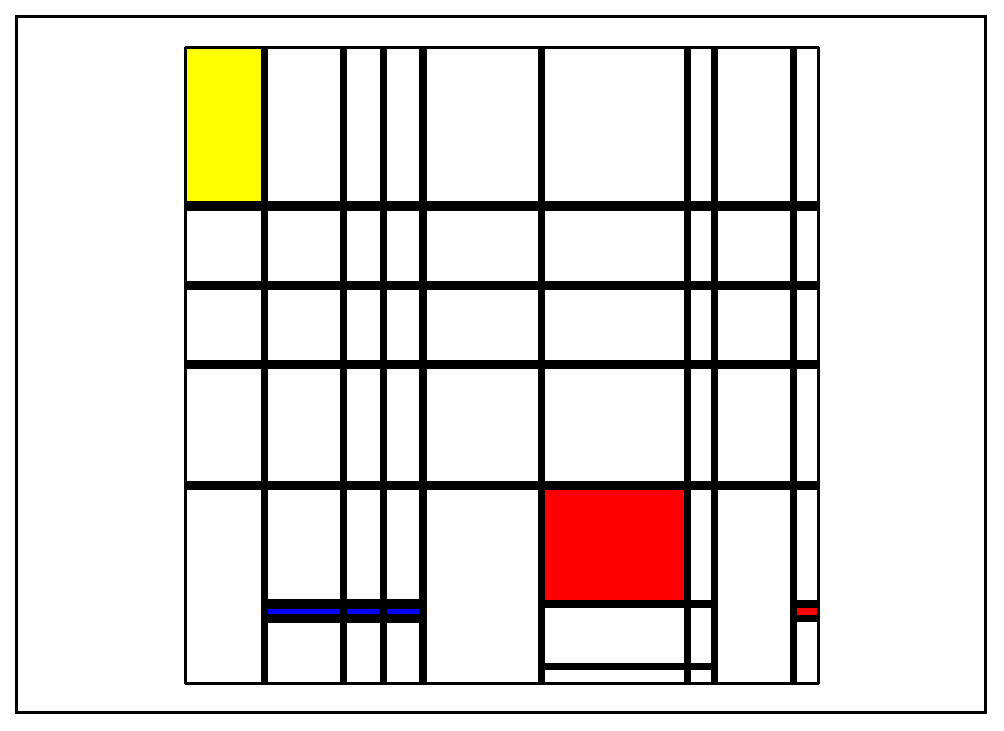
\includegraphics[width=\textwidth]{mondrian1}\\
Et voici la suite d'instructions :
\begin{verbatim}
rectangle(6i,1+6i,2,affichage=rempli+3);
rectangle(1+0.8i,3+0.8i,1/10,affichage=rempli+4);
rectangle(9/2+i,6.33+i,0.8,affichage=rempli+1);
segment(1+0.8i,3+0.8i, affichage=epaisseur_ligne_4);;
segment(1+1*i,3+1*i, affichage=epaisseur_ligne_4);;
segment(5i/2,8+5i/2,affichage=epaisseur_ligne_4);;
segment(3,3+8*i,affichage=epaisseur_ligne_3);;
segment(5i,8+5i,affichage=epaisseur_ligne_4);;
segment(6i,8+6i,affichage=epaisseur_ligne_4);;
segment(1,1+8i,affichage=epaisseur_ligne_3);;
segment(2,2+8i,affichage=epaisseur_ligne_3);;
segment(5/2,5/2+8i,affichage=epaisseur_ligne_3);;
segment(3,3+8i,affichage=epaisseur_ligne_3);;
segment(9/2,9/2+8i,affichage=epaisseur_ligne_3);;
segment(19/3,19/3+8i,affichage=epaisseur_ligne_3);;
segment(20/3,20/3+8i,affichage=epaisseur_ligne_3);;
segment(23/3,23/3+8i,affichage=epaisseur_ligne_3);
segment(9/2+i,20/3+i,affichage=epaisseur_ligne_3);
segment(9/2+0.2i,20/3+0.2i,affichage=epaisseur_ligne_3);
segment(4i,8+4i,affichage=epaisseur_ligne_4);;
rectangle(23/3+0.8*i,8+0.8*i,6/10,affichage=rempli+1);
segment(23/3+0.8i,8+0.8i, affichage=epaisseur_ligne_3);;
segment(23/3+1*i,8+1*i, affichage=epaisseur_ligne_3);;
segment(23/3,23/3+8i,affichage=epaisseur_ligne_3);;
carre(0,8);
\end{verbatim}
\section{Grandeurs proportionnelles}
On dit que $y$ et $x$ sont proprotionnels si $y/x$ est \'egales \`a une 
constante $a$ qui s'appelle le coefficient de proportionnalit\'e.\\
Par exemple le prix $y$ d'un tissu est proportionnel \`a sa 
longueur $x$.\\
{\bf Exercice}
Un pain de 400g est vendu dans un supermarch\'e 0.85 euros.\\
Sur l'\'etiquette il est marqu\'e :
Prix au kilo 1.89 euros.\\
\begin{itemize}
\item
Si ce prix au kilo \'etait exact quel devrait \^etre le prix de ce pain 
de 400g?\\
\item
Si ce prix au kilo \'etait exact quel devrait \^etre le poids de ce pain 
qui coute 0.85 euros ?\\
\item Quel est le prix r\'eel au kilo ?
\end{itemize}
{\bf Solution}
\begin{itemize}
\item 1 kilo=1000 grammes et 400 grammes=0.4 kilo.\\
Si 1 kilo coute 1.89 euros cela veut dire que le prix $y$ en euros est 
proportionnel au poids $x$ du pain en kilo et que le coefficient de
 proportionnalit\'e vaut 1.89 et on a $y=1.89*x$\\
Donc un pain 400grammes=0.4 kilos doit couter :\\
1.89*0.4=0.756 euros, soit environ 0.76 euros.
\item si le prix $y$ vaut 0.85 euros c'est que le poids $x$ de ce pain 
v\'erifie la relation $0.85=1.89*x$ donc :\\
$x=0.85/1.89=0.449735449735$\\
Le poids de ce pain devrait \^etre d'environ 450 grammes.
\item Le prix r\'eel au kilo est \'egal \`a $y/x$ c'est \`a dire \`a :\\
0.85/0.4=2.125 euros.
\end{itemize}
\section{Pourcentage}
\subsection{Devis HT et TTC}
Un artisan doit faire un devis qu'il estime \`a 500 euros HT (hors taxes).\\
A combien se monte le devis avec la TVA si celle-ci est de 19.6\%.

Le montant de la TVA est :\\
500*19.6*0.01=500*0.196=98
Le montant TTC est donc:\\
500+98 =598 euros\\
ou bien directement; le montant TTC est :\\
500*1.196=598 euros\\

Un artisan a fait un devis d'un montant de 600 euros TTC (avec la TVA).\\
A combien se monte le devis HT (hors taxes) si la TVA  est de 19.6\% ?
si la TVA  est de 7\% ?

Si la TVA  est de 19.6\%, le montant HT est donc de :\\
600/1.196=501.67 euros.\\ 
Si la TVA  est de 7\%, le montant HT est donc de :\\
600/1.07=560.74 euros.
\subsection{Placement sur un livret}
On place sur un livret la somme de 10000 euros \`a un taux annuel d'int\'er\^et 
de 2.5\% (net d'imp\^ots de de taxes).\\
Les int\'er\^ets \'etant vers\'es sur le livret, quelle somme a-t-on obtenue au 
bout d'un an sur le livret? \\
Au bout d'un an, par combien la somme initiale a-t-elle \'et\'e multipli\'ee ?\\
Quelle somme a-t-on obtenue au bout de 2 ans ? 5 ans ? 
 
Au bout d'un an, on a  10000*2.5/100= 10000*0.025=250 euros d'int\'er\^ets donc 
au total on a sur le livret : 10000+10000*0.025=10000*1.025=10250 euros.\\
Au bout d'un an, la somme initiale a-t-elle \'et\'e multipli\'ee par 1.025.\\
Au bout de 2 ans, on a  10250*0.025=256.25 euros d'int\'er\^ets donc au total on 
a sur le livret : 10250+256.25=10506.25 euros ou encore \\
le total se monte \`a $10000*1.025*1.025=10000*1.025^2=10506.25$ euros.\\
Au bout de  5 ans, on a  $10000*1.025^5=11314.08$ euros sur le livret.\\
On place sur un livret la somme de $S$ euros \`a un taux annuel d'int\'er\^et 
de $t*0.01$ (net d'imp\^ots de de taxes).\\
Quelle somme a-t-on obtenue au bout d'un an ? \\
Les int\'er\^ets \'etant vers\'es sur le compte, ils rapportent aussi des 
int\'er\^et.\\
Quelle somme a-t-on obtenue au bout de $n$ ans ? \\ 

\noindent Au bout d'un an on a : $S*(1+t*0.01)$ euros\\
Au bout de $n$ ans on a : $S*(1+t*0.01)^n$ euros\\
\section{Cercle et Arc de cercle}
Voici les commandes de {\tt Xcas} qui permettent de faire un cercle :\\
{\tt cercle} ou {\tt circle} permet de d\'efinir un cercle et un arc de cercle.
{\tt arc} permet de d\'efinir un arc par 2 points et son angle au centre.
 Si on veut dessiner un cercle {\tt cercle} ou {\tt circle} a 1 ou 2 arguments :
\begin{itemize}
\item son \'equation.\\ 
Par exemple {\tt cercle((x-1)\verb|^|2+(y-2)\verb|^|2=1)} 
\item son centre et son rayon le centre \'etant un point
et le rayon un nombre r\'eel.\\
Par exemple : {\tt cercle(point(1,2),1)}
\item son diam\`etre : les arguments sont alors 2 points.\\
Par exemple : {\tt cercle(point(1,2),point(0,3))}
\end{itemize}
Si on veut dessiner un arc de cercle $AB$ on utilise :
\begin{enumerate} 
\item {\tt cercle} ou {\tt circle} a 4 arguments
\begin{itemize}
\item son centre, son rayon et les angles aux centres des points $A$ et $B$ 
(les arguments sont alors un point (pour le centre), 3 nombres r\'eels pour le 
rayon et les 2 angles au centre. C'est l'axe d\'efinit par le diam\`etre qui d\'etermine l'origine pour la mesure des angles au centre.\\
Par exemple : {\tt cercle(point(1,2),1,pi/4,pi/2)}
\item son diam\`etre  et les angles aux centres des points $A$ et $B$ (les arguments sont alors 2 points et 2 nombres r\'eels).\\
Par exemple : {\tt cercle(point(1,2),point(0,3),pi/6,2pi/3)}\\
{\bf Attention}
{\tt cercle(point(0,3),point(1,2),pi/6,2pi/3)} et {\tt cercle(point(1,2),point(0,3),pi/6,2pi/3)} sont des arcs sym\'etriques par rapport au diam\`etre
\end{itemize}
\item {\tt arc} avec 3,4 ou 5 arguments
\begin{itemize}
\item les 3 arguments sont 2 points qui sont les  extr\'emit\'es de l'arc et 
l'angle au centre.\\
Par exemple : {\tt arc(point(1,2),point(0,3),pi/2)}
\item avec 4 ou 5 arguments, on rajoute le nom d'1 ou 2 variables qui donneront
le centre et le rayon du cercle contenant cet arc.\\ 
Par exemple : {\tt arc(point(1,2),point(0,3),pi/2,C)} dessinne l'arc et le point {\tt C} qui est le centre du cercle supportant l'arc ({\tt coordonnees(C)} renvoie {\tt [0,2]}) ou\\
{\tt arc(point(1,2),point(0,3),pi/2,C,r)}
dessinne l'arc et le point {\tt C} qui est le centre du cercle supportant l'arc ({\tt coordonnees(C)} renvoie {\tt [0,2]}) et {\tt r} renvoie {\tt 1}.
\end{itemize}
\end{enumerate}
{\bf Remarque}\\
On peut rajouter un dernier argument aux commandes tr\'ec\'edentes pour g\'erer
l'affichage par exemple :\\
{\tt cercle(point(1,2),point(0,3),pi/6,2pi/3,affichage=rempli+4)}\\
{\tt  arc(point(1,2),point(0,3),pi/2,affichage=rempli+1)}
\section{Reproduction d'un tableau de Robert Delaunay}
Voici Disque de Robert Delaunay reproduit avec {\tt Xcas}:\\
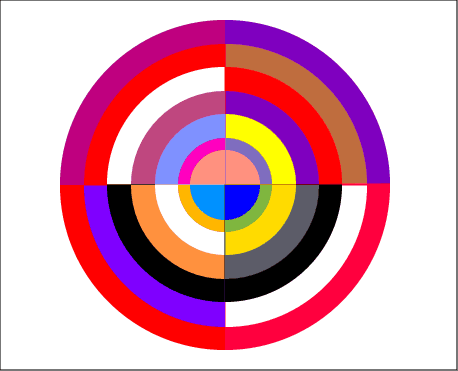
\includegraphics[width=\textwidth]{delaunay}
\begin{verbatim}
cercle(0,7,0,pi/2,affichage=rempli+192);
cercle(0,6,0,pi/2,affichage=rempli+123);
cercle(0,5,0,pi/2,affichage=rempli+88);
cercle(0,4,0,pi/2,affichage=rempli+192);
cercle(0,3,0,pi/2,affichage=rempli+95);
cercle(0,2,0,pi/2,affichage=rempli+195);
cercle(0,1.5,0,pi/2,affichage=rempli+172);
cercle(0,7,pi/2,pi,affichage=rempli+160);
cercle(0,6,pi/2,pi,affichage=rempli+88);
cercle(0,5,pi/2,pi,affichage=rempli+7);
cercle(0,4,pi/2,pi,affichage=rempli+164);
cercle(0,3,pi/2,pi,affichage=rempli+236);
cercle(0,2,pi/2,pi,affichage=rempli+208);
cercle(0,1.5,pi/2,pi,affichage=rempli+172);
cercle(0,7,pi,3pi/2,affichage=rempli+88);
cercle(0,6,pi,3pi/2,affichage=rempli+232);
cercle(0,5,pi,3pi/2,affichage=rempli);
cercle(0,4,pi,3pi/2,affichage=rempli+132);
cercle(0,3,pi,3pi/2,affichage=rempli+7);
cercle(0,2,pi,3pi/2,affichage=rempli+93);
cercle(0,1.5,pi,3pi/2,affichage=rempli+220);
cercle(0,7,3pi/2,pi*2,affichage=rempli+128);
cercle(0,6,3pi/2,pi*2,affichage=rempli+7);
cercle(0,5,3pi/2,pi*2,affichage=rempli);
cercle(0,4,3pi/2,pi*2,affichage=rempli+24);
cercle(0,3,3pi/2,pi*2,affichage=rempli+94);
cercle(0,2,3pi/2,pi*2,affichage=rempli+117);
cercle(0,1.5,3pi/2,pi*2,affichage=rempli+216);
\end{verbatim}

\chapter{Statistiques}

\section{S\'erie statistique donn\'ee par une liste}\index{count\_eq}\index{\$}
\index{alea}\index{pour}\index{NULL}\index{fpour}\index{jusque}\index{append}
\index{diagramme\_batons}\index{histogramme}\index{count\_eq}
On jette 2 d\'es cubiques non pip\'es et on note la somme obtenue dans une 
liste {\tt R}.\\
Simuler ce jet 25 fois de suite \`a l'aide de {\tt Xcas}.\\
Calculer les fr\'equences de chaque issue et construire l'histogramme (i.e. le 
diagramme en b\^atons) correspondant.\\
Simuler ce lancer 40 fois de suite \`a l'aide du tableur de {\tt Xcas}.\\
Simuler ce lancer 1000 fois de suite \`a l'aide de {\tt Xcas}.\\
Calculer les fr\'equences de chaque issue et constriure le diagramme en 
b\^atons correspondant.\\

Avec {\tt Xcas}, on tape dans une ligne de commande :\\
{\tt R:=[]; pour j de 1 jusque 25 faire R:=append(L,alea(6)+alea(6)+2);fpour;}\\
ou bien on tape :\\
{\tt R:=[(alea(6)+alea(6)+2)\$(k=1..25)]}\\
En effet {\tt alea(6)} renvoie  un nombre choisi al\'eatoirement parmi
les nombres {\tt 0,1,2,3,4,5} donc {\tt alea(6)+1} renvoie
 un nombre choisi al\'eatoirement parmi les nombres {\tt 1,2,3,4,5,6}.\\ 
{\bf Attention} {\tt alea(6)+alea(6)+2} n'est pas \'egal \`a {\tt 2*alea(6)+2} 
et n'est pas \`egal non plus \`a {\tt alea(11)+2}.\\
Puis on utilise {\tt count\_eq(k,R)} qui compte le nombre d'\'el\'ements de la 
liste {\tt R} égaux à {\tt k} pour {\tt k} allant de 0 \`a 12 et on tape :\\
{\tt [count\_eq(k,R)\$(k=0..12)]}\\
Ou bien on tape directement :\\
{\tt L:=[0\$ 13]}
cela cr\'ee une liste form\'ee de 13 z\'eros.\\
{\tt R:=NULL;}\\
cela cr\'ee une s\'equence vide\\
{\tt pour j de 1 jusque 25 faire k:=alea(6)+alea(6)+2;R:=R,k;L[k]:=L[k]+1;fpour;}\\ 
cela effectue 25 jets de 2 d\'es et on cr\'ee la s\'equence {\tt R} qui donne 
la suite des r\'esultats et la liste {\tt L} qui compte dans {\tt L[k]} le 
nombre de fois que {\tt k} a \'et\'e obtenu.\\
{\tt R:=[R];}\\
cela transforme la s\'equence  {\tt R} en une liste.\\
On obtient par exemple pour {\tt R}:\\ 
{\tt [7,8,8,3,10,5,9,4,2,7,9,6,5,10,7,7,6,6,7,4,4,4,9,5,8]}\\
On obtient alors pour {\tt L}:\\ 
{\tt [0,0,1,1,4,3,3,5,3,3,2,0,0]}\\
Les frequences sont donc {\tt L/25}. 
On obtient \\
{\tt [0,0,1/25,1/25,4/25,3/25,3/25,1/5,3/25,3/25,2/25,0,0]}\\
On tape :\\
{\tt histogramme([[k,L[k]]\$(k=0..12)])}\\
Ou on tape :\\
{\tt histogramme(R,0.5,1)}
On obtient :\\ 
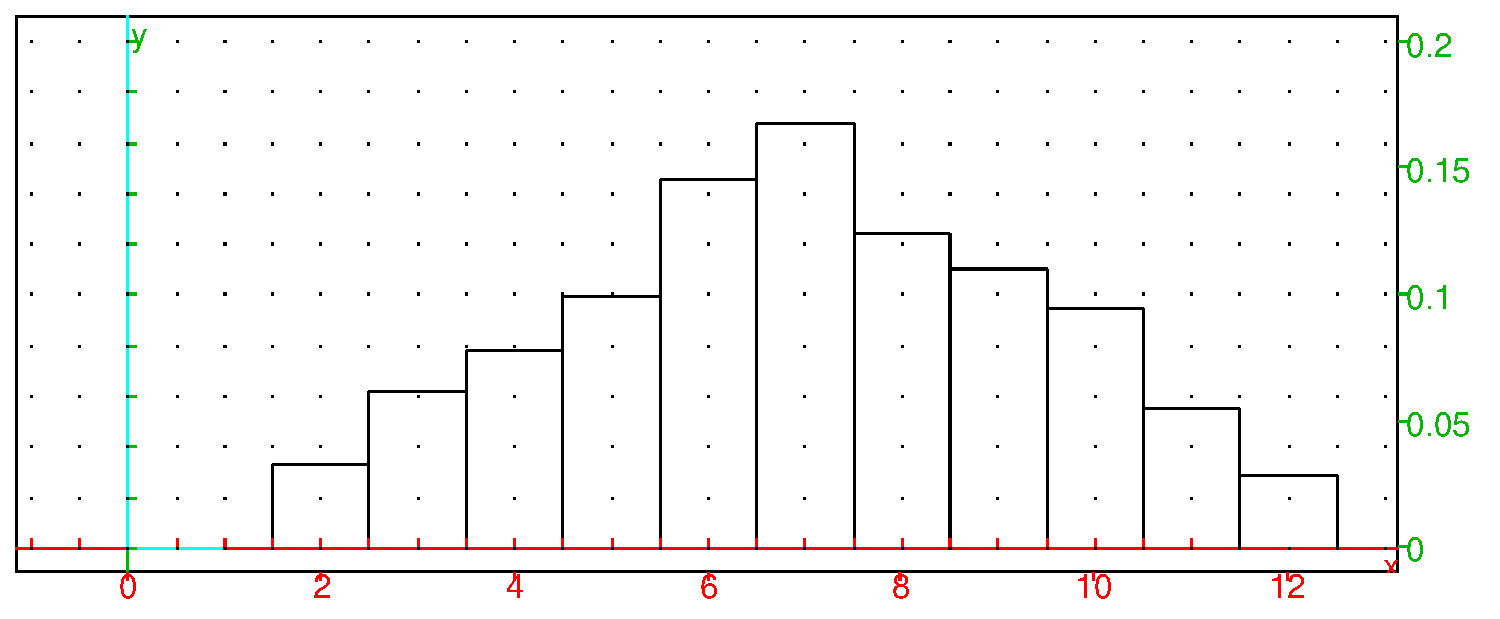
\includegraphics[width=\textwidth]{troishist}\\
ou bien on tape :\\
{\tt diagramme\_batons([[k,L[k]]\$(k=0..12)])}\\
On obtient :\\ 
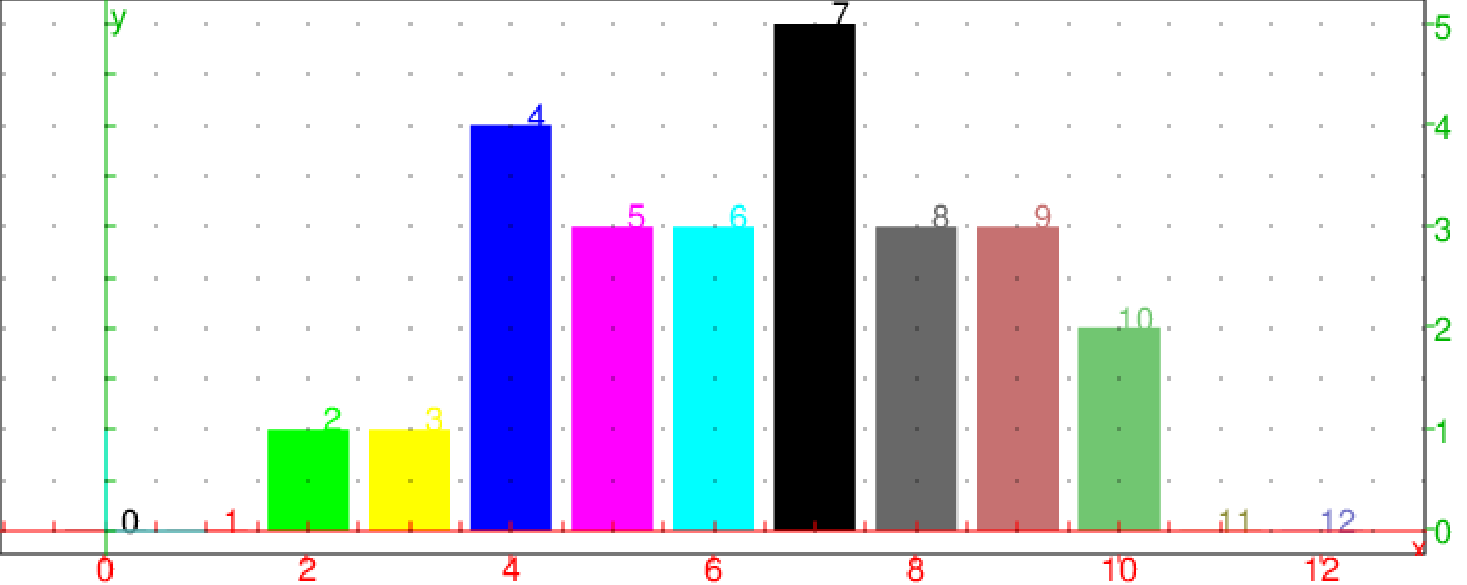
\includegraphics[width=\textwidth]{troisbat}\\
{\bf Avec le tableur}
On ouvre le tableur avec par exemple avec :\\
{\tt Alt+t}\\
 ou avec le menu :
{\tt Tableur->Nouveau tableur}\\
qio propose 40 lignes de 0 \`a 39. On appuie donc sur {\tt OK
Dans {\tt A} on met les nombres entiers 0,1..39 :\\
pour cela on met dans {\tt A0} : {\tt 0} et dans {\tt A1} : {\tt =A0+1} \\
puis on s\'electionne {\tt A1} et on tape {\tt Ctrl+d} pour remplir 
vers le bas.\\
Dans {\tt B} on met le r\'esultat des 40 jets :\\
pour cela on met dans {\tt B0} : {\tt alea(6)+alea(6)+2}\\
puis on s\'electionne {\tt B0} et on tape {\tt Ctrl+d} pour remplir vers 
le bas.\\
Dans {\tt C2} on va mettre le nombre de fois qu'il y a 2 dans {\tt B} et
dans {\tt C3} on mettre le nombre de fois qu'il y a 3 dans {\tt B} etc...\\
Pour cela, on tape dans {\tt C2} :{\tt =count\_eq(A2,[\$B\$0:\$B\$39])} puis 
on s\'electionne {\tt C2} et on tape {\tt Ctrl+d} pour remplir 
vers le bas.\\
Dans le menu {\tt Maths} du tableur, on s\'electionne :\\
{\tt stats-1d->diagramme\_batons} et on met {\tt A2:A12,C} dans plage de 
cellule et {\tt D0} comme cellule cible.\\
On obtient dans \tt D0} : {\tt =diagramme\_batons([[2,1],...[12,0]])} \\
et  sous le tableur (ou \`a c\^ot\'e si on a d\'ecoch\'e 
{\tt Paysage}) le graphique :\\
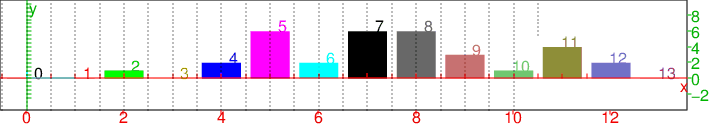
\includegraphics[width=\textwidth]{trisbatab}\\
{\bf Pour 1000 lancers},\\
 on tape directement dans une ligne de commande :\\
{\tt LL:=[0\$ 13]}
{\tt pour j de 1 jusque 1000 faire k:=alea(6)+alea(6)+2;LL[k]:=LL[k]+1;fpour;}\\ 
On obtient :\\ 
{\tt [0,0,33,62,78,100,146,168,124,110,95,55,29]}\\
Les 2 premiers 0 signifient que le score obtenu en jetant 2 d\'es n'est jamais 
nul et jamais \'egal \`a 1, puis 33 signifie que 2 a \`et\'e obtenu 33 fois 
lorsqu'on a fait 1000 lancers etc...\\
Les fr\'equences sont donc {\tt LL/1000}\\
On obtient \\
{\tt [0,0,33/1000,31/500,39/500,1/10,73/500,21/125,31/250,11/100,19/200,11/200,29/1000]}\\
On tape :\\
{\tt evalf(LL/1000,3)}\\
On obtient :\\
{\tt [0.0,0.0,0.033,0.062,0.078,0.1,0.146,0.168,0.124,0.11,0.095,0.055,0.029]}\\
On tape :\\
{\tt histogramme([[k,LL[k]]\$(k=0..12)])}\\
On obtient :\\ 
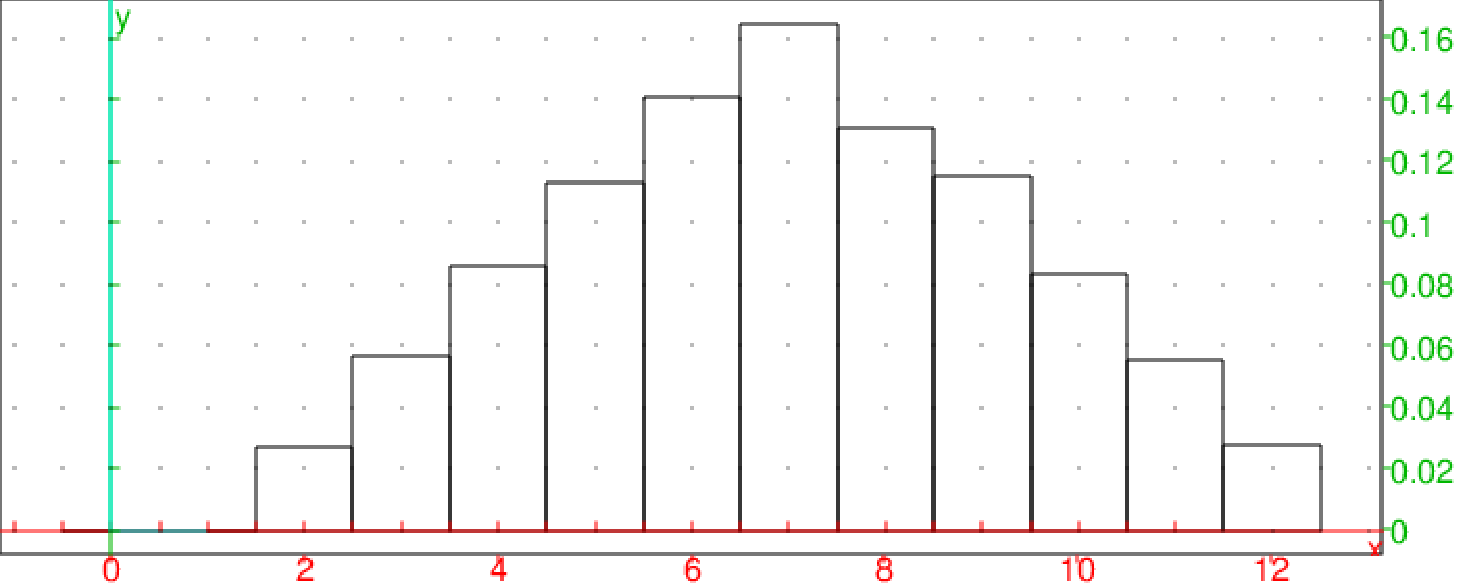
\includegraphics[width=\textwidth]{troishist1}\\
On peut aussi utiliser :\\
{\tt =diagramme\_batons([[k,LL[k]]\$(k=0..12)])}\\
{\bf Calcul \`a la main les fr\'equences th\'eoriques}\\
Il y a en tout $6^2=36$ possibilit\'es.\\
Calculons parmi ces 36 possibilit\'es combien ont comme somme 2,
ont comme somme 3,...,ont comme somme 12 :
\begin{itemize}
\item 2 est obtenu si on a fait (1,1) donc 1 fois
\item 3 est obtenu si on a fait (1,2) ou (2,1) donc 2 fois
\item 4 est obtenu si on a fait (1,3), (2,2) ou (3,1) donc 3 fois
\item 5 est obtenu si on a fait (1,4), (2,3), (3,2) ou (4,1) donc 4 fois
\item 6 est obtenu si on a fait (1,5), (2,4), (3,3), (4,2) ou (5,1) donc 5 fois
\item 7 est obtenu si on a fait (1,6), (2,5), (3,4), (4,3), (5,2) ou (6,1) donc
 6 fois
\item 8 est obtenu si on a fait (2,6), (3,5), (4,4) (5,3) ou (6,2) donc 5 fois
\item 9 est obtenu si on a fait  (3,6), (4,5) (5,4) ou (6,3) donc 4 fois
\item 10 est obtenu si on a fait (4,6) (5,5) ou (6,4) donc 3 fois
\item 11 est obtenu si on a fait (5,6) ou (6,5) donc 2 fois
\item 12 est obtenu si on a fait (6,6) donc 1 fois
\end{itemize}
On v\'erifie (1+2+3+4+5)*2+6=36\\
Les fr\'equences th\'eoriques de 2,3,4,5,6,7,8,9,10,11,12  sont donc:\\
{\tt 1/36, 1/18, 1/12, 1/9, 5/36, 1/6, 5/36, 1/9, 1/12, 1/18, 1/36 }
On tape :\\
{\tt evalf([1/36,1/18,1/12,1/9,5/36,1/6,5/36,1/9,1/12,1/18,1/36],3)}\\ 
On obtient :\\
{\tt [0.028,0.056,0.083,0.111,0.139,0.167,0.139,0.111,0.083,0.056,0.028]}
\section{S\'erie statistique donn\'ee par un tableau ou un graphique}
\chapter{Probabilit\'es}
\section{\'Equiprobabilit\'e}\index{alea}\index{rand}\index{min}\index{max}\index{trier}
On jette 3 d\'es \`a 6 faces. On suppose que ces 3 d\'es ne sont pas pip\'es 
(i.e. il y  a \'equiprobabilit\'e d'obtenir chaque face)\\
On ordonne par ordre croissant les 3 valeurs obtenues : $m,d,M$.\\
$A$ gagne si $M-m>d$ et sinon c'est $B$ qui gagne.\\
Le jeu est-il \'equitable ?

Il y a $6^3=$ possibilit\'es il faut calculer le nombres de possibilit\'es qui
correspondent \`a  $M-m>d$.\\
On peut faire cela avec un programme en utilisant les fonctions :\\
{\tt alea} ou {\tt  rand}, {\tt max} et {\tt min} de {\tt Xcas} :\\
{\tt a:=rand(6)+1;b:=rand(6)+1;c:=rand(6)+1;} donne les 3 valeurs obtenues\\
{\tt M:=max(a,b,c); m:=min(a,b,c);} calcule le maximum {\tt M} et le minimum 
{\tt m} de ces 3 valeurs,\\
{\tt d:=a+b+c-M-m;} calcule le terme m\'edian puisque $M+d+m=a+b+c$.\\
On tape :\\
\begin{verbatim}
destrois(n):={
 local M,m,d,a,b,c,j,p;
 pour j de 1 jusque n faire 
   a:=rand(6)+1;
   b:=rand(6)+1;
   c:=rand(6)+1;
   M:=max(a,b,c);
   m:=min(a,b,c);
   d:=a+b+c-M-m;
   si M-m<d alors p:=p+1 fsi;
   fpour;
  retourne(p/n);
  }:;
\end{verbatim}
On peut aussi utiliser une s\'equence et la fonction {\tt trier} qui trie par 
ordre croissant.
On tape :\\
\begin{verbatim}
destroiss(n):={
 local M,m,d,S,j,p;
 pour j de 1 jusque n faire 
   S:=trier(rand(6)+1,rand(6)+1,rand(6)+1);
   m:=S[0];
   d:=S[1];
   M:=S[2];
   si M-m<d alors p:=p+1 fsi;
   fpour;
  retourne(p/n);
  }:;
\end{verbatim}
On tape :\\
{\tt destrois(10000)}\\
On obtient :\\
{\tt 5105/10000}\\
On tape :\\
{\tt destrois(100000)}\\
On obtient :\\
{\tt 51247/1000000}\\
\begin{verbatim}
probadestrois():={
 local M,m,d,a,b,c,p;
 pour a de 1 jusque 6 faire 
  pour b de 1 jusque 6 faire 
   pour c de 1 jusque 6 faire 
    M:=max(a,b,c);
    m:=min(a,b,c);
    d:=a+b+c-M-m;
    si M-m<d alors p:=p+1 fsi;
   fpour;
  fpour;
 fpour;
 retourne(p/6^3);
  }:;
\end{verbatim}
Ou bien on tape :
\begin{verbatim}
probadestroiss():={
 local M,m,d,a,b,c,p,S;
 pour a de 1 jusque 6 faire 
  pour b de 1 jusque 6 faire 
   pour c de 1 jusque 6 faire 
    S:=trier(a,b,c);
    m:=S[0];
    d:=S[1];
    M:=S[2];
    si M-m<d alors p:=p+1 fsi;
   fpour;
  fpour;
 fpour;
 retourne(p/6^3);
  }:;
\end{verbatim}
On tape :\\
{\tt probadestrois()}\\
ou 
{\tt probadestroiss()}\\
On obtient :\\
{\tt 37/72 ($\simeq$ 0.513888888889)}\\
{\bf Calcul \`a la main}\\
Il y a en tout $6^3=216$ possibilit\'es.\\
Calculons le nombre de cas favorables pour que $A$ gagne.\\
\begin{itemize}
\item Si $M-m=5$ on doit avoir $M-m=5<d$ donc $d=6$  les 3 possibilit\'es sont
(1,6,6) (6,1,6) et (6,6,1). Ce qui fait en tout 3 possibilit\'es.
\item Si $M-m=4$ on doit avoir $M-m=4<d$ donc $d=6$ ou $d=5$. 
 \begin{itemize}
\item Si  $d=6$  3 possibilit\'es (2,6,6),
\item si $d=5$ (1,5,5) soit 3 possibilit\'es ou (2,5,6) soit 3!=6 
possibilit\'es. 
\end{itemize}
Ce qui fait en tout 3+3+6=12 possibilit\'es.
\item Si $M-m=3$ on doit avoir $M-m=3<d$ donc $d=6$ ou $d=5$ ou $d=4$. 
\begin{itemize}
\item Si $d=6$ 3 possibilit\'es (3,6,6), 
\item si $d=5$ (2,5,5) 3 possibilit\'es ou (3,5,6) soit 3!=6 possibilit\'es,
\item si $d=4$ (1,4,4) 3 possibilit\'es ou (2,4,5) 3!=6 possibilit\'es ou 
(3,4,6) 3!=6 possibilit\'es.
 \end{itemize}
Ce qui fait en tout 3*3+3*6=27 possibilit\'es.
\item Si $M-m=2$ on doit avoir $M-m=2<d$ donc $d=6$ ou $d=5$ ou $d=4$ ou $d=3$.
\begin{itemize}
\item si $d=6$ 3 possibilit\'es (4,6,6), 
\item si $d=5$ (3,5,5) 3 possibilit\'es ou (4,5,6) soit 6 possibilit\'es, 
\item si $d=4$ (2,4,4) 3 possibilit\'es ou (3,4,5) 6 possibilit\'es ou (4,4,6) 
3 possibilit\'es,
 \item si $d=3$ (1,3,3) 3 possibilit\'es ou (2,3,4) 6 possibilit\'es ou (3,3,5) 3 possibilit\'es. 
\end{itemize}
Ce qui fait en tout 4*3+5*6=36 possibilit\'es.
 \item Si $M-m=1$ on doit avoir $M-m=1<d$ donc $d=6$ ou $d=5$ ou $d=4$ ou $d=3$ ou 
$d=2$. 
\begin{itemize}
\item Si $d=6$ 3 possibilit\'es (5,6,6), 
\item si $d=5$ (4,5,5) 3 possibilit\'es ou (5,5,6) soit 3 possibilit\'es, 
\item si $d=4$ (3,4,4) 3 possibilit\'es ou (4,4,5) 3 possibilit\'es, 
\item si $d=3$ (2,3,3) 3 possibilit\'es ou 
(3,3,4) 3 possibilit\'es,
\item  si  $d=2$  (1,2,2) 3 possibilit\'es ou (2,2,3) 3 possibilit\'es.
\end{itemize}
 Ce qui fait en tout 3*9=27 possibilit\'es.
\item  Si $M-m=0$ on doit avoir $M-m=0<d$ donc $M=m=d$ et $d=6$ ou $d=5$ ou $d=4$ ou $d=3$ ou $d=2$ ou $d=1$.  Ce qui fait en tout 6 possibilit\'es.
\end{itemize}
On fait le total soit :\\
3+12+27+36+27+6=111 cas possibles.
Donc la probabilit\'e pour $A$ de gagner est :\\
{\tt 111/216} on obtient {\tt 37/72}
\section{La loterie "illico SOLITAIRE" et le tableur}
La loterie "illico SOLITAIRE" consiste \`a acheter, pour 2 euros, un ticket 
faisant partie d'un bloc de 750 000 tickets. Pour ce bloc il y a :
\begin{verbatim}
100000 lots de     2 euros
 83000 lots de     4 euros
 20860 lots de     6 euros
  5400 lots de    12 euros
  8150 lots de    20 euros
   400 lots de   150 euros
    15 lots de  1000 euros
     2 lots de 15000 euros
\end{verbatim}
Calculer \`a l'aide  de {\tt Xcas} :\\
La probabilit\'e de gagner une somme sup\'erieur ou \'egale \`a 500 euros 
Mettre les donn\'ees dans le tableur de {\tt Xcas} et faites apparaitre :
\begin{itemize}
\item le nombre de tickets gagnants
\item la valeur en euros de tous les tickets gagnants
\item la moyenne des gains
\item le pourcentage de tickets gagnants
\end{itemize}
Combien avez-vous de chances de gagner ? (gagner signifiant avoir un lot 
sup\'erieur \`a sa mise)\\
Ce jeu vous parait-il \'equitable ?\\

{\bf La solution}\\
Dans la colonne $A$ on met le nombre de tickets gagnants et dans 
la colonne $B$ la valeur en euros de ces tickets.\\
On tape donc dans $A_0$ 100000 et dans $B0$ 2 etc...\\ 
Le nombre de tickets gagnant est la somme : $A_0+A_1+... A_{10}$.
Pour cela on remplit la colonne $C$ et on met :\\
dans $C_0$ : $A_0$\\
dans $C_1$ : $=C_0+A_1$\\
et on remplit vers le bas.\\
En $C_7$ on lit 217827, ce qui repr\'esente le nombre de tickets gagnants.\\

Pour avoir la somme des lots de tous les tickets gagnants, on remplit la 
colonne $D$  et on met :\\
dans $D_0$ : $A_0*B_0$\\
dans $D_1$ : $=D0+A_1*B_1$\\
et on remplit vers le bas.\\
En $D_7$ on lit 989960, ce qui repr\'esente la valeur en euros de tous les 
tickets gagnants.\\
La moyenne des gains est \'egale \`a : \\
989960/750000.=1.31994666667 euros\\

Le pourcentage de tickets gagnants est \'egale \`a :\\
{\tt evalf(217827/750000)} soit 0.290436.\\
Ce pourcentage est sup\'erieur \`a 0.25 donc il y a plus d'une chance sur 4 
d'avoir un ticket gagnant. MAIS, il y a 100000 tickets gagnants de 2 euros, 
soit des tickets qui repr\'esentent pour le parieur un gain nul ! \\
Donc le pourcentage de tickets gagnants un lot sup\'erieur \`a sa mise
est \'egale \`a :\\
{\tt evalf(117827/750000)} soit 0.157102666667.\\
On peut donc dire que le parieur \`a 15.7102666667 chances sur 100 de gagner 
plus que sa mise de 2 euros.\\
Celui qui organise cette loterie, si il vend tous les tickets du bloc, gagne :\\
{\tt 750000*2- 989960} soit 510040 euros !\\
Soit $X$ la variable al\'eatoire \'egale au gain possible.\\
 $X$ peut prendre les valeurs :\\
-2 avec une probabilit\'e de $1-217827/750000=177391/250000$\\
0 avec une probabilit\'e de $100000/750000=2/15$\\
2  avec une probabilit\'e de $83000/750000=83/750$\\
4  avec une probabilit\'e de $20860/750000=1043/37500$\\
10  avec une probabilit\'e de $5400/750000=9/1250$\\
18  avec une probabilit\'e de $8150/750000=163/15000$\\
148  avec une probabilit\'e de $ 400/750000=1/1875$\\
998   avec une probabilit\'e de $15 /750000=1/50000$\\
14998  avec une probabilit\'e de $2/750000=1/375000$\\ 
Donc l'esp\'erance de $X$ est donc \'egale \`a :\\
$E(X)=-2*177391/250000+2*83/750+4*1043/37500+10*9/1250+18*163/15000+
148*1/1875+998*1/50000+14998*1/375000=-12751/18750\simeq -0.680053333333$
Donc l'esp\'erance de gain est une perte de 0.68 euros.\\
0n retrouve le r\'esultat pr\'ec\'edent puisque on mise 2 euros et que la 
moyenne des gains est \'egale \`a 989960/750000 euros ($\simeq 1.31994666667$ 
euros, soit une perte moyenne (989960/750000-2)=-12751/18750 euros soit environ
de -0.68 euros.

\section{La loterie "CAS-H illico" et le tableur}
La loterie "CAS-H illico" consiste \`a acheter, pour 5 euros, un ticket 
faisant partie d'un bloc de 15 000 000 tickets. Pour ce bloc il y a :
\begin{verbatim}
1560000 tickets gagnants de      5 euros 
1760000 tickets gagnants de     10 euros 
 375000 tickets gagnants de     20 euros 
 112500 tickets gagnants de     50 euros 
 112500 tickets gagnants de    100 euros 
   3750 tickets gagnants de    500 euros 
   1800 tickets gagnants de   1000 euros 
     40 tickets gagnants de   5000 euros 
      5 tickets gagnants de  10000 euros 
      3 tickets gagnants de 100000 euros  
      3 tickets gagnants de 500000 euros 
\end{verbatim}
Calculer \`a l'aide  de {\tt Xcas} :\\
La probabilit\'e de gagner une somme sup\'erieur ou \'egale \`a 500 euros 
Mettre les donn\'ees dans le tableur de {\tt Xcas} et faites apparaitre :
\begin{itemize}
\item le nombre de tickets gagnants
\item la valeur en euros de tous les tickets gagnants
\item la moyenne des gains
\item le pourcentage de tickets gagnants
\end{itemize}
Voici la publicit\'e de la loterie "CAS-H illico" :\\
"Plus d'1 chance sur 4 de gagner !"\\
Qu'en pensez-vous ?\\
Ce jeu vous parait-il \'equitable ?\\

{\bf La solution}\\
Dans la colonne $A$ on met le nombre de tickets gagnants et dans 
la colonne $B$ la valeur en euros de ces tickets.\\
On tape donc dans $A_0$ 1560000 et dans $B0$ 5 etc...\\ 
Le nombre de tickets gagnant est la somme : $A_0+A_1+... A_{10}$.
Pour cela on remplit la colonne $C$ et on met :\\
dans $C_0$ : $A_0$\\
dans $C_1$ : $=C_0+A_1$\\
et on remplit vers le bas.\\
En $C_{10}$ on lit 3925601, ce qui repr\'esente le nombre de tickets gagnants.\\

Pour avoir la somme des lots de tous les tickets gagnants, on remplit la 
colonne $D$ et on met :\\
dans $D_0$ : $A_0*B_0$\\
dans $D_1$ : $=D0+A_1*B_1$\\
et on remplit vers le bas.\\
En $D_{10}$ on lit 55500000, ce qui repr\'esente la valeur en euros de tous les 
tickets gagnants.\\
La moyenne des gains est \'egale \`a : \\
55500000/15000000=37/10=3.7 euros\\

Le pourcentage de tickets gagnants est \'egale \`a :\\
{\tt evalf(3925601/15000000)} soit 0.261706733333.\\
Ce pourcentage est sup\'erieur \`a 0.25 donc il y a plus d'une chance sur 4 
d'avoir un ticket gagnant. MAIS, il y a 1560000 tickets gagnants de 5 euros, 
soit des tickets qui repr\'esentent pour le parieur un gain nul ! \\
Puisque 1-0.261706733333=0.738293266667, on peut donc dire que le parieur \`a
 73.8293266667 chances sur 100 de perdre 5 euros\\
Puisque 1560000/15000000.=0.104, on peut donc dire que le parieur \`a
10.4 chances sur 100 de ne rien gagner et de ne rien perdre.\\
Le pourcentage de tickets gagnants une somme sup\'erieure strictement \`a 
5 euros est \'egale \`a :\\
{\tt evalf((3925601-1560000)/15000000)} soit 0.157706733333.\\ 
On peut donc dire que le parieur \`a 15.7706733333 chances sur 100 de gagner 
plus que sa mise de 5 euros.\\
Celui qui organise cette loterie, si il vend tous les tickets du bloc, gagne :\\
{\tt 15000000*5-55500000} soit 19500000 euros !\\
Soit $X$ la variable al\'eatoire \'egale au gain possible.\\
 $X$ peut prendre les valeurs :\\
-5 avec une probabilit\'e de $1-3925601/15000000=11074399/15000000$\\
0 avec une probabilit\'e de $1560000/15000000=13/125$\\
5  avec une probabilit\'e de $1760000/15000000=44/375$\\
15  avec une probabilit\'e de $375000/15000000=1/40$\\
45  avec une probabilit\'e de $112500/15000000=3/400$\\
95  avec une probabilit\'e de $112500/15000000=3/400$\\
495  avec une probabilit\'e de $ 3750/15000000=1/4000$\\
995   avec une probabilit\'e de $1800 /15000000=3/25000$\\
4995   avec une probabilit\'e de $40/15000000=1/375000$\\
9995 avec une probabilit\'e de $5/15000000=1/3000000$
99995  avec une probabilit\'e de $3/15000000=1/5000000$\\ 
499995 avec une probabilit\'e de $3/15000000=1/5000000$\\
Donc l'esp\'erance de $X$ est donc \'egale \`a :\\
$E(X)=-5*11074399/15000000+5*44/375+15*1/40+45*3/400+95*3/400+
495*1/4000+995*3/25000+4995*1/375000+9995*1/3000000+99995*1/5000000+
499995*1/5000000=-13/10$
Donc l'esp\'erance de gain est une perte de 1.30 euros.\\
0n retrouve le r\'esultat pr\'ec\'edent puisque on mise 5 euros et que la 
moyenne des gains est \'egale \`a 3.7 euros, soit une perte moyenne de 
-1.30 euros.

\section{Pour comprendre l'\'ecart type}
\subsection{Un exercice}
Le comit\'e des f\^etes d'un village veut organiser une loterie en \'emettant 
1000 billets \`a 2 euros.\\
{\bf A}\\ 
Le comit\'e des f\^etes h\'esite entre 3 possibilit\'es quand aux lots 
possibles :\\
\begin{enumerate}
\item il y a 10 billets qui gagnent 102 euros
\item il y a 43 billets qui gagnent 3,4,..32,33,33,34,...44 euros
\item il y a 100 billets qui gagnent 10.2 euros
\end{enumerate}
Soient $X_1,X_2,X_3$ les variables al\'eatoires \'egales au gain (en euros) du 
joueur qui ach\'ete 1 billet pour chacune des 3 possibilit\'es.\\
Pour chacune des 3 possibilit\'es calculer la moyenne et l'\'ecart type de 
cette variable al\'eatoire.\\
{\bf B}\\ 
Apr\`es un sondage Le comit\'e des f\^etes d\'ecide d'opter pour la premi\`ere 
solution :\\
sur 1000 billets \`a 2 euros il y a 10 billets qui gagnent 102 euros.\\
\begin{enumerate}
\item 2 amis d\'ecident d'acheter ensemble 2 billets et de se partager les 
gains car ils estiment qu'il auront plus de chances de gagner. Est-ce vrai ?\\
Soit $X_4$ la variable al\'eatoire \'egales au gain (en euros) d'un des 2 amis. 
Calculer la moyenne et l'\'ecart type de cette variable al\'eatoire $X_4$.
\item m\^eme question pour $n$ ($n=2..1000)$ amis d\'ecident d'acheter ensemble
 $n$ billets et de se partager les gains
\item Les comit\'es des f\^etes de 100 villages organisent le m\^eme type de 
loterie: 1000 billets de 2 euros avec 10 lots de 102 euros. Un habitant d'un 
village voisin d\'ecide de miser 
\begin{itemize}
\item 20  euros\\
A-t-il inter\^et \`a acheter les billets de loterie d'un m\^eme village ou 
des billets de loterie de villages tous diff\'erents ?
Calculer pour chacun des cas la moyenne et l'\'ecart type de ces gains.
\item 200  euros\\
M\^eme question.
Faire un graphique qui compare les probabilit\'e d'avoir $k$  ($k=0..10$) 
billets gagnants sur les 100 billets achet\'es.
\end{itemize}
\end{enumerate}
\subsection{La solution de A}
\begin{itemize}
\item il y a 10 billets qui gagnent 102 euros $X_1$ peut prendre 2 valeurs :\\
 -2 avec la probabilit\'e de 99/100 ou \\
100 (102-2=100) avec la probabilit\'e de 1/100 $simeq$ 0.01.\\
Donc pour calculer la moyenne $m_1=E(X_1)$, on tape :\\
{\tt  m1:=-2*99/100+100*1/100}\\
On obtient :\\ 
{\tt  -49/50}$\simeq$ {\tt -0.98}\\
Donc pour calculer l'\'ecart type $\sigma(X_1)$, on tape :\\
{\tt  sqrt((-2-m1)\verb|^|2*99/100+(100-m1)\verb|^|2*1/100)}\\
On obtient :\\ 
{\tt  7650*sqrt(11)/2500}$\simeq$ {\tt  10.1488718585}
\item il y a 43 billets qui gagnent 3,4,..32,33,33,34,...44 euros
$X_2$ peut prendre 43 valeurs :\\
 -2 avec la probabilit\'e de 957/1000 ou \\
1,2..30 avec la probabilit\'e de 1/1000\\
31 (33-2=31) avec la probabilit\'e de 2/1000\\
32..42 avec la probabilit\'e de 1/1000\\
Donc pour calculer la moyenne $m_2=E(X_2)$, on tape :\\
{\tt m2:=-2*957/1000+sum(n,n=1..30)*1/1000+31*2/1000+\\
          sum(n,n=32..42)*1/1000}\\
On obtient :\\ 
{\tt  -49/50}$\simeq$ {\tt -0.98}\\
Donc pour calculer l'\'ecart type $\sigma(X_2)$, on tape :\\
{\tt sqrt((-2-m2)\verb|^|2*957/1000+sum((n-m2)\verb|^|2,n=1..30)*1/1000+\\
     (31-m2)\verb|^|2*2/1000+sum((n-m2)\verb|^|2,n=32..42)*1/1000)}\\
On obtient :\\ 
{\tt  25*sqrt(73534)/1250}$\simeq$ {\tt 5.42343064858}
\item il y a 100 billets qui gagnent 10.2 euros
$X_3$ peut prendre 2 valeurs : \\
-2 avec la probabilit\'e de 9/10 ou\\
 8.2 (10.2-2=8.2) avec la probabilit\'e de 1/10
Donc pour calculer la moyenne $m_3=E(X_3)$, on tape :\\
{\tt  m3:=-2*9/10+8.2*1/10}\\
On obtient :\\ 
{\tt  -0.98}\\
Donc pour calculer l'\'ecart type $\sigma(X_3)$, on tape :\\
{\tt  sqrt((-2-m3)\verb|^|2*9/10+(8.2-m3)\verb|^|2*1/10)}\\
On obtient :\\ 
{\tt  3.06}
\end{itemize}
On remarque que dans les 3 cas les moyennes sont les m\^emes mais par contre 
les \'ecarts types sont diff\'erents : ils sont de plus en plus petits au
fur et \`a mesure que l'on a plus de chances d'avoir un billet gagnant en effet
\`a moyenne \'egale si on a plus de chances d'avoir un billet gagnant c'est que
le gain est plus petit et donc l'\'ecart des gains \`a la moyenne est plus petit
car l'\'ecart type r\'esume les \'ecarts entre chaque r\'esultat possible et 
la valeur moyenne.\\
Dans tous les 3 cas la vente de tous les billets rapportera au comit\'e des 
f\^etes la somme de 980 euros. Mais que faut-il pr\'ef\'erer peu de gros 
lots ou beaucoup de petits lots ? \`A vous de choisir !!!!\\
\subsection{La solution de B}
Sur 1000 billets \`a 2 euros il y a 10 billets qui gagnent 102 euros.\\
\begin{enumerate}
\item 2 amis d\'ecident d'acheter ensemble 2 billets et de se partager les gains.\\
Soit $X_4$ la variable al\'eatoire\'egale au gain obtenu par l'un d'eux,
$X_4$ peut prendre les valeurs :\\
\begin{itemize}
\item -2 avec la probabilt\'e :\\
{\tt comb(990,2)/comb(1000,2)}$\simeq$ 0.98009009009
\item (102-4)/2=49 avec la probabilt\'e :\\
{\tt comb(990,1)*comb(10,1)/comb(1000,2)}$\simeq$ 0.0198198198198
\item 100 avec la probabilt\'e :\\
{\tt comb(10,2)/comb(1000,2)}$\simeq$ 9.00900900901e-05
\end{itemize}
Donc pour $n=2$\\
En misant 2 euros on a une chance de gagner en se mettant \`a 2, avec une 
probabilit\'e de 0.0199099099099 (au lieu de 0.01) mais le gain risque d\^etre 
moins important !
Pour calculer la moyenne $m_4=E(X_4)$, on tape :\\
{\tt m4:=(-2*comb(990,2)+49*comb(990,1)*comb(10,1)+\\
100*comb(10,2))/comb(1000,2)}\\
On obtient encore la m\^eme moyenne :\\ 
{\tt -49/50}$\simeq$ -0.98\\
Pour calculer l'\'ecart type $\sigma(X_4)$, on tape :\\
{\tt  sqrt(((-2-m4)\verb|^|2*comb(990,2)+(49-m4)\verb|^|2*comb(990,1)*\\comb(10,1)+(100-m4)\verb|^|2*comb(10,2))/comb(1000,2))}\\
On obtient :\\ 
{\tt 850*sqrt(609279)/92500}$\simeq$ 7.17274345342.\\
\item $n$ amis d\'ecident d'acheter ensemble $n$ billets et de se partager les 
gains.\\
Ce qu'il faut comprendre c'est que si $n$ ($n\leq 1000$) parieurs d\'ecident de
partager le gain provenant des $n$ billets de cette loterie, l'esp\'erance de 
gain d'un joueur sera toujours de -0.98 (c'est \`a dire une perte de -0.98 
euros) mais l'\'ecart type sera de plus en plus petit au fur et \`a mesure que 
$n$ augmente : le cas limite \'etant $n=1000$ avec un gain s\^ur de -0.98 euros
et donc un \'ecart type nul.
{\bf  La solution de B pour $n=2..1000$ avec un programme}\\
On doit regarder 3 cas diff\'erents :
\begin{itemize}
\item $1<=n<=10$\\
Dans ce cas le nombre $p$ de billets gagnants peut \^etre $0,1..n$
\item $11<=n<=990$\\
Dans ce cas le nombre $p$ de billets gagnants peut \^etre $0,1..10$
\item $991<=n<=1000$\\
Dans ce cas le nombre $p$ de billets gagnants peut \^etre $n-990..10$
\end{itemize}
On tape pour calculer dans chacun de ces cas la moyenne et l'\'ecart type de la 
variable al\'eatoire \'egale au gain d'un parieur :\\
\begin{verbatim}
msigma(n):={
local p,m,sigma2;
m:=0;
sigma2:=0;
si n<=10 alors 
  pour p de 0 jusque n faire
    m:=m+(102*p-2*n)/n*comb(990,n-p)*comb(10,p)/comb(1000,n);
  fpour;
  pour p de 0 jusque n faire
    sigma2:=sigma2+((102*p-2*n)/n-m)^2*comb(990,n-p)*comb(10,p)/
                    comb(1000,n);
  fpour;
sinon
  si n<=990 alors 
    pour p de 0 jusque 10 faire
      m:=m+(102*p-2*n)/n*comb(990,n-p)*comb(10,p)/comb(1000,n);
    fpour;
    pour p de 0 jusque 10 faire
      sigma2:=sigma2+((102*p-2*n)/n-m)^2*comb(990,n-p)*comb(10,p)/
                      comb(1000,n);
    fpour;
  sinon
    pour p de n-990 jusque 10 faire
      m:=m+(102*p-2*n)/n*comb(990,n-p)*comb(10,p)/comb(1000,n);
    fpour;
    pour p de n-990 jusque 10 faire
      sigma2:=sigma2+((102*p-2*n)/n-m)^2*comb(990,n-p)*comb(10,p)/
                      comb(1000,n);
    fpour;
  fsi;
fsi;
retourne [m,sqrt(sigma2)];
}:;
\end{verbatim}
Pour $n$ fix\'e, on appelle $mn$ la moyenne et $sn$ l'\'ecrat type et on trace 
les points d'abscisse $n$ et d'ordonn\'ee $sn/mn$ (c'est le coefficient de 
dispersion) :
\begin{verbatim}
gmsigma():={
  local L,n,msn,mn,sn;
  L:=NULL;
   pour n de 1 jusque 1000 faire
    msn:=msigma(n);mn:=evalf(msn[0]);sn:=evalf(msn[1]);
    L:=L,point(n,sn/mn,affichage=1);
   fpour;
 retourne L;
}:;  
\end{verbatim}
On tape :\\
{\tt gmsigma()}\\
On obtient le coefficient de dispersion en fonction de $n$ :\\
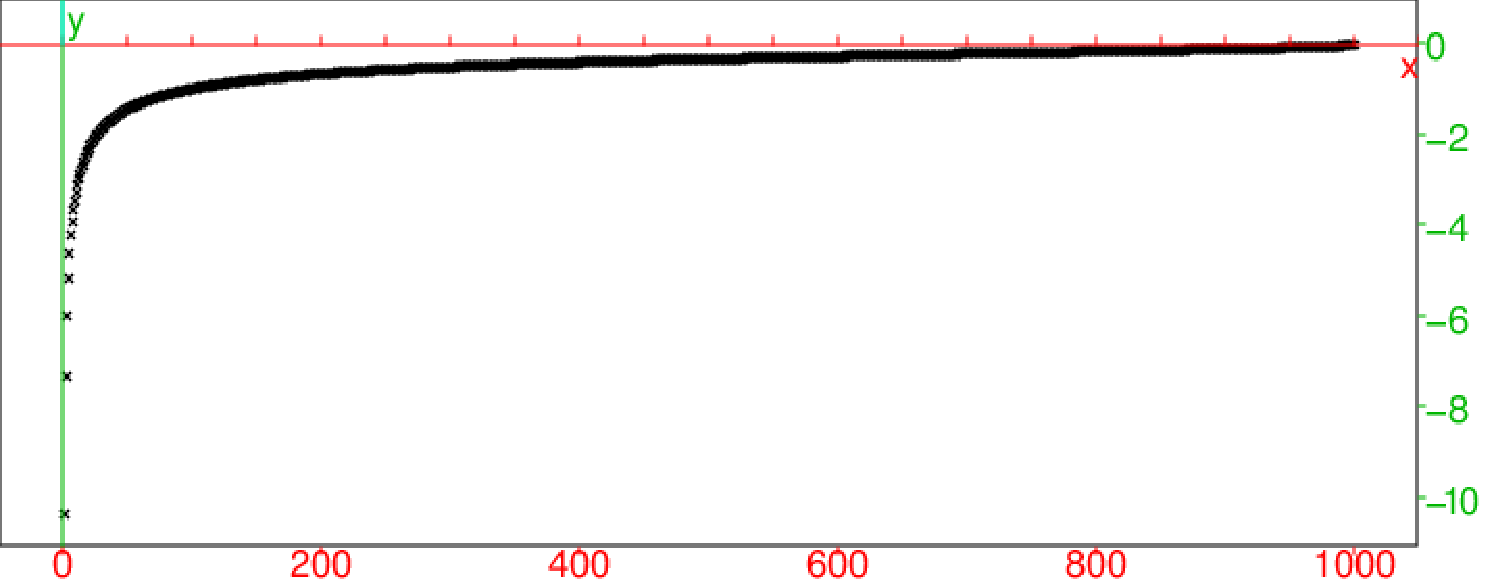
\includegraphics[width=\textwidth]{ecartype}\\
\item Les comit\'es des f\^etes de 100 villages organisent le m\^eme type de 
loterie : 1000 billets de 2 euros avec 10 lots de 102 euros.
\begin{itemize}
\item Un habitant d'un village voisin d\'ecide de miser 20  euros\\
Si il ach\`ete 10 billets de la  loterie du m\^eme village :\\
Soit $X_5$ la variable al\'eatoire \'egale au gain du parieur.\\
$X_5$ a 11 valeurs possibles qui sont : $102*k-20$ pour $k=0..10$\\
Chacune de ces valeurs a une probabilit\'e \`egale \`a :\\
{\tt comb(10,k)*comb(990,10-k)/comb(1000,10)} pour $k=0..10$\\
On tape :\\
{\tt V5:=[(102*k-20)\$(k=0..10)]}\\
On obtient:\\
{\tt [-20,82,184,286,388,490,592,694,796,898,1000]}\\
On tape :\\
{\tt P5:=[(comb(10,k)*comb(990,10-k)/comb(1000,10))\$(k=0..10)]}\\
On obtient pour {\tt evalf(P5,4)} :\\
{\tt [0.904,0.09215,0.0038,8.248e-05,1.027e-06,7.505e-09,3. 172e-11,7.345e-14,8.363e-17,3.758e-20,3.796e-24]}\\
La moyenne $m_5$ vaut :\\
{\tt moyenne(V5,P5)} soit {\tt -49/5}\\
L'\'ecart type $\sigma_5$ vaut :\\
{\tt ecart\_type(V5,P5)} soit {\tt 2805*sqrt(111)/925}$\simeq$ 31.948658137

Si il ach\`ete 10 billets de la loterie de 10 villages diff\'erents :\\
Chaque billet \`a une probabilit\'e de 1/100 d\^etre gagnant car les 10 tirages
sont ind\'ependants : il s'agit alors de la loi binomiale $B(10,1/100)$.
Soit $X_6$ la variable al\'eatoire \'egale au gain du parieur.\\
$X_6$ a 11 valeurs possibles : les m\^emes que $X_5$ et donc :\\
{\tt V6:=V5}\\
Chacune de ces valeurs a une probabilit\'e \`egale \`a  :\\
{\tt binomial(10,k,1/100)=comb(10,k)*(1/100)\verb|^|k*(99/100)\verb|^|(10-k)}
On tape pour vair la probabilit\'e des 11 premi\`eres valeurs :\\
{\tt P6:=[binomial(10,k,1/100)\$(k=0..10)]}\\
On obtient pour {\tt evalf(P5,4)} :\\
{\tt [0.9044,0.09135,0.004152,0.0001118,1.977e-06,2.396e-08, 2.017e-10,1.164e-12,4.41e-15,9.9e-18,1e-20]}
La moyenne $m_6$ vaut :\\
{\tt moyenne(V6,P6)} soit {\tt -49/5}\\
L'\'ecart type $\sigma_6$ vaut :\\
{\tt ecart\_type(V6,P6)} soit {\tt 765*sqrt(110)/250}$\simeq$ 32.093550754\\
\item Un habitant d'un village voisin d\'ecide de miser 200  euros\\
Il ach\`ete 100 billets de la loterie du m\^eme village :\\
Soit $X_7$ la variable al\'eatoire \'egale au gain du parieur.\\
$X_7$ a 11 valeurs possibles qui sont : $102*k-200$ pour $k=0..10$\\
Chacune de ces valeurs a une probabilit\'e \`egale \`a :\\
{\tt comb(10,k)*comb(990,100-k)/comb(1000,100)} pour $k=0..10$\\
On tape :\\
{\tt V7:=[(102*k-200)\$(k=0..10)]}\\
On obtient:\\
{\tt [-200,-98,4,106,208,310,412,514,616,718,820]}\\
On tape :\\
{\tt P7:=[(comb(10,k)*comb(990,100-k)/comb(1000,100))\$(k=0..10)]}\\
On obtient  pour {\tt evalf(P7,4)} :\\
{\tt [0.3469,0.3894,0.1945,0.05691,0.01081,0.001391,0.0001229,7.359e-06,2.858e-07,6.499e-09,6.572e-11]}\\
La moyenne $m_7$ vaut :\\
{\tt moyenne(V7,P7)} soit {\tt -98}\\
L'\'ecart type $\sigma_7$ vaut :\\
{\tt ecart\_type(V7,P7)} soit {\tt 102*sqrt(1221)/37}$\simeq$ 96.3288287235

Si il ach\`ete 100 billets de la loterie de 100 villages diff\'erents :\\
Chaque billet \`a une probabilit\'e de 1/100 d\^etre gagnant car les 100 tirages
sont ind\'ependants : il s'agit alors de la loi binomiale $B(100,1/100)$.
Soit $X_8$ la variable al\'eatoire \'egale au gain du parieur.\\
$X_8$ a 101 valeurs possibles car chaque billet peut gagner (bien que peu probable !) :\\
{\tt V8:=[(102*k-200)\$(k=0..101)]:;}\\
Chacune de ces valeurs a une probabilit\'e \`egale \`a  :\\
{\tt binomial(100,k,1/100)}
On tape :\\
{\tt P8:=[binomial(100,k,1/100)\$(k=0..101)]:;}\\
On obtient pour les 14 premi\`eres valeurs approch\'ees de {\tt evalf(P8,4)} :\\
{\tt [0.366,0.3697,0.1849,0.061,0.01494,0.002898,0.0004635,6.286e-05,7.382e-06,7.622e-07,7.006e-08,5.79e-09,4.338e-10,2.966e-11]]}
La moyenne $m_8$ vaut :\\
{\tt moyenne(V8,P8)} soit {\tt -98}\\
L'\'ecart type $\sigma_8$ vaut :\\
{\tt ecart\_type(V8,P8)} soit {\tt 765*sqrt(11)/25}$\simeq$ 101.488718585\\

On compare les probabilit\'es d'avoir $k=0..10$ billets gagnants.\\
On tape :\\
{\tt  [point(V7[k],P7[k],affichage=epaisseur\_point\_2)\$(k=0..10),
point(V8[k],P8[k],affichage=1+point\_plus+epaisseur\_point\_2)\\
\$(k=0..10)]}\\
On obtient en rouge la loi binomiale :\\
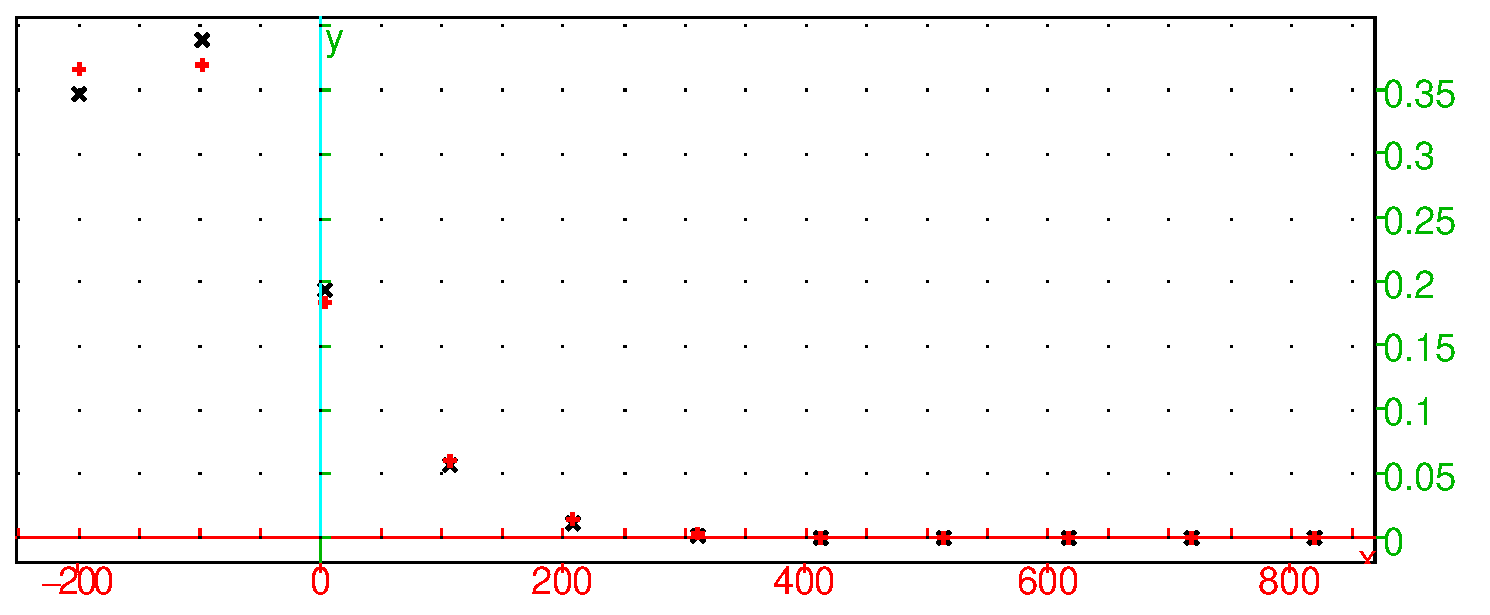
\includegraphics[width=\textwidth]{ecartbi}
\end{itemize}
\end{enumerate}
%\section{Arbre pour mod\'eliser une exp\'erience al\'eatoire}
%\chapter{Th\'eor\`eme de Thal\'es}
%\section{Calcul d'une longueur}
%\section{D\'emontrer que 2 droites sont parall\`eles}
\chapter{Trigonom\'etrie-Angles-Polygones}
\section{Longueur d'un c\^ot\'e d'un triangle rectangle}\index{pa2b2}\index{longueur}\index{segment}\index{triangle}\index{polygone}\index{plotparam}
\subsection{Exercice 1}
On peut montrer que si $p$ est un nombre premier qui a 1 comme reste lorsqu'on
le divise par 4 alors il existe deux entiers $a$ et $b$ tels que $p=a^2+b^2$.\\
{\bf Application}
$p=61$, $p=153$.\\
Factoriser $n=388$ et d\'ecomposer $n$ en une somme de 2 carr\'es.\\
Construire le triangle $ABC$ tel que 
 $BC=a=\sqrt{388}$, , $AC=b=\sqrt{61}$, $AB=c=\sqrt{153}$.\\
D\'eterminer l'aire de $ABC$.\\
Inventer un exercice semblable \`a celui la.\\
{\bf La solution}
On v\'erifie que 61 et 153 sont premiers et ont 1 comme reste lorsqu'on les 
divise par 4 :\\
\begin{itemize}
\item 61 n'est pas divisible par 2,3,5,7 et comme $11^2=121>61$ on en d\'eduit 
que 61 est un nombre premier.\\
0n a : 61=4*15+1 
\item 153 n'est pas divisible par 2,3,5,7,11 et comme $13^2=169>153$ on en 
d\'eduit que 153 est un nombre premier.\\
0n a : 153=4*38+1 
\end{itemize}
On trouve par tatonnement que :\\
$61=25+36=5^2+6^2$\\
$153=9+144=3^2+12^2$\\
Ou bien on utilise la fonction {\tt pa2b2} de {\tt Xcas} qui fait cette 
d\'ecomposition. {\tt pa2b2(p)} renvoie la liste $[a,b]$ tel que $p=a^2+b^2$
On tape {\tt pa2b2(61)} et on obtient {\tt [6,5]}\\
On tape {\tt pa2b2(153)} et on obtient {\tt [12,3]}\\
On factorise 388, on tape :\\
{\tt factoriser\_entier(388)} et on obtient {\tt 2\verb|^|2*97}\\
On  v\'erifie que 97 est premier et a 1 comme reste lorsqu'on le divise par 4 :
97 n'est pas divisible par 2,3,5,7 et comme $11^2=121>97$ on en d\'eduit 
que 97 est un nombre premier.\\
On a  : 97=4*24+1.\\
Donc 97 se d\'ecompose en une somme de 2 carr\'es.\\
On trouve par tatonnement que :\\
$97=16+81=4^2+9^2$\\
Ou bien on tape {\tt pa2b2(97)} et on obtient {\tt [9,4]}\\ 
Donc $388=4*(4^2+9^2)=8^2+18^2$\\
Pour construire le triangle $ABC$, on sait d'apr\`es le th\'eor\`eme de 
Pythagore et les r\'esultats pr\'ec\'edent que :
$BC=a=\sqrt{388}$ est l'hypoth\'enuse d'un triangle rectangle de c\^ot\'es de 
longueur 8 et 18,\\
$AC=b=\sqrt{61}$ est l'hypoth\'enuse d'un triangle rectangle de c\^ot\'es de 
longueur 5 et 6,\\ 
$AB=c=\sqrt{153}$ est l'hypoth\'enuse d'un triangle rectangle de c\^ot\'es de 
longueur 3 et 12.\\
On remarque que 8=5+3 et que 18=6+12, d'o\`u la construction dans un niveau de 
g\'eom\'etrie $2d$ :
\begin{verbatim}
B:=point(18);
C:=point(0,8);
A:=point(6,3);
triangle (A,B,C);
segment(A,6,affichage=2);
segment(A,point(0,3),affichage=2);
\end{verbatim}
On obtient :\\
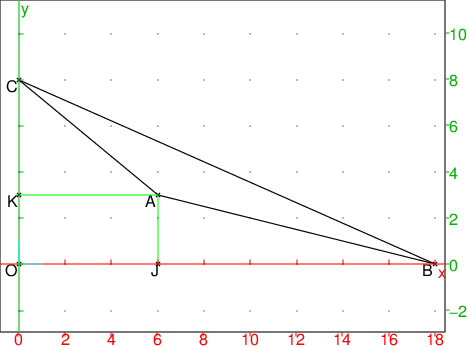
\includegraphics[width=\textwidth]{troistri}\\
On tape pour v\'erifier :\\
{\tt longueur2(B,C),longueur2(A,C),longueur2(A,B)}\\
On obtient :\\
{\tt 388,61,153}\\
L'aire du triangle $ABC$ se calcule facilement par diff\'erence :\\
aire de $OBC$ est \'egale \`a 18*8/2=72.\\
aire de $KAC$ est \'egale \`a 5*6/2=15.\\
aire de $OBAK$ est \'egale \`a 3*(18+6)/2=3*12=36.\\
Donc l'aire du triangle $ABC$ est \'egale \`a 72-15-36=21.\\
On  v\'erifie avec {\tt Xcaqs}, on tape :\\
{\tt aire(triangle(A,B,C))}\\
On obtient :\\
{\tt 21}\\
Pour faire un exercice de m\^eme style, il faut choisir d'avoir
la m\^eme configuration pour la construction du triangle $ABC$.\\
Par exemple :\\
$OB=2+8=10$, $OC=1+5=6$ et $A$ le point de coordonn\'ees (2,1).\\
On a alors :\\
$BC^2=100+36=136$\\
$AC^2=4+25=29$\\
$AB^2=1+64=65$\\
et  l'aire du triangle $ABC$ est \'egale \`a 19.
\subsection{Exercice 2}
Soient dans le plan, un rectangle $ABCD$ et un point $M$ \`a l'int\'erieur 
du rectangle.\\
Les parall\`eles aux c\^ot\'es du rectangle passant par $M$ coupent :\\
$AB$ en $P$, $BC$ en $Q$, $CD$ en $R$ et $AD$ en $S$.\\
On pose $a=AP$, $b=PB$, $c=AS$ et $d=SD$.\\
Calculer $MA^2$, $MB^2$, $MC^2$. $MD^2$ en fonction de $a,b,c,d$\\
Calculer $MC^2$ en fonction de $MA^2$, $MB^2$, $MD^2$.\\
Application num\'erique :\\
On donne $MA=9$, $MB=7$ et $MD=6$\\
Calculer $MC$\\
On veut d\'eterminer les  rectangles $ABCD$ ayant cette propri\'et\'e \`a 
savoir $MA=9$, $MB=7$ $MC=2$ et $MD=6$ pour un point $M$ du plan $ABC$.\\ 
Pour cela on note :\\
$x=a^2$, $y=b^2$, $z=c^2$ et $t=d^2$.\\
D\'eterminer le syst\`eme lin\'eaire que v\'erifie $x,y,z,t$\\
R\'esoudre ce syst\`eme lin\'eaire avec {\tt Xcas}.\\
Construire un rectangle $ABCD$ ayant cette propri\'et\'e.\\
{\bf La solution}\\
On ouvre un niveau de g\'eom\'etrie 2-d.\\
On tape :\\
\begin{verbatim}
A:=point(0);
B:=point(5);
C:=point(5+i*3);
D:=point(i*3);
polygone(A,B,C,D);
M:=point(4+i);
P:=point(4);
R:=point(4+3*i);
S:=point(i);
Q;=point(5+i);
segment(A,M);
segment(B,M);
segment(C,M);
segment(D,M);
segment(P,R);
segment(S,Q);
segment(A,P,affichage=1),
point(2,legend="a",affichage=1)
segment(B,P,affichage=2),
point(4.5,legend="b",affichage=2)
segment(A,S,affichage=4),
point(i/2,legend="c",affichage=4)
segment(D,S,affichage=5),
point(i*2,legend="d",affichage=5)
\end{verbatim}
On obtient :\\
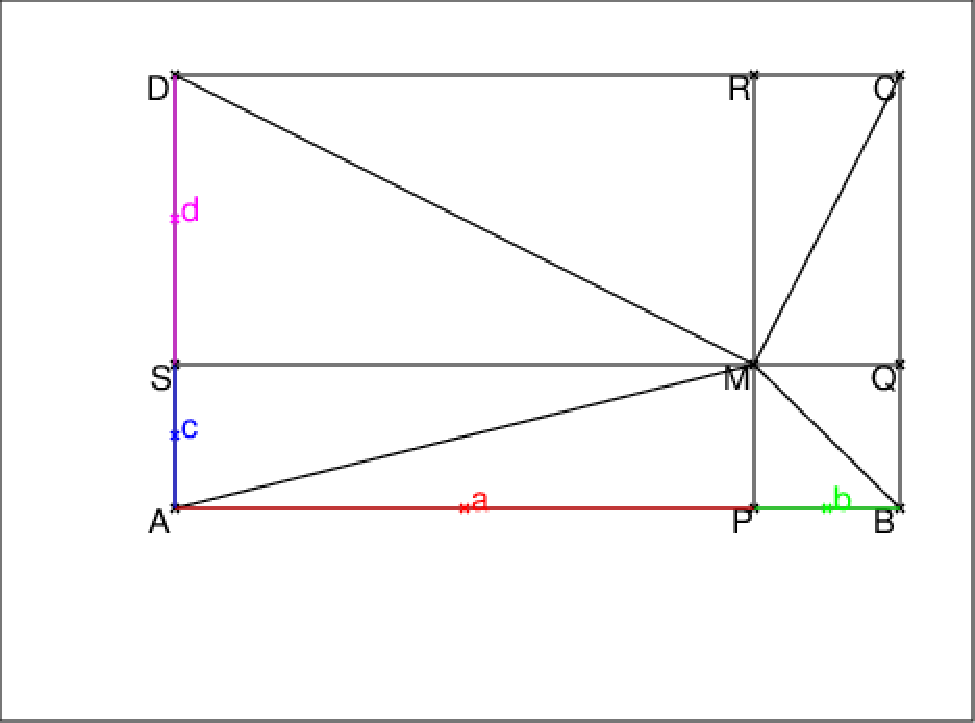
\includegraphics[width=\textwidth]{troisrect}\\

On a d'apr\`es Pythagore :\\
$AM^2=a^2+c^2$\\
$BM^2=b^2+c^2$\\
$CM^2=b^2+d^2$\\
$DM^2=a^2+d^2$\\
Donc :\\
$AM^2+CM^=a^2+c^2+b^2+d^2$\\
$BM^2+DM^2=b^2+c^2+a^2+d^2$\\
Donc $AM^2+CM^=BM^2+DM^2$\\
On en d\'eduit :\\
$CM^2=BM^2+DM^2-AM^2$
On remarquera que cette relation est enore valable si $M$ se trouve \`a 
l'ext\'erieur du rectangle $ABCD$.\\
Application num\'erique :\\
$CM^2=49+36-81=4$
Donc $CM=2$\\

Soit maintenant un rectangle $ABCD$ et un point $M$ du plan $ABC$.\\
Les parall\`eles aux c\^ot\'es du rectangle passant par $M$ coupent :\\
$AB$ en $P$, $BC$ en $Q$, $CD$ en $R$ et $AD$ en $S$.\\
On pose  $a=AP$, $b=PB$, $c=AS$ et $d=SD$.\\
On a d'apr\`es ce qui pr\'ec\`ede :\\
$AM^2=a^2+c^2=81$\\
$BM^2=b^2+c^2=49$\\
$CM^2=b^2+d^2=4$\\
$DM^2=a^2+d^2=36$\\
c'est \`a dire si $x=a^2,y=b^2,z=c^2,t=d^2$:\\
x+z=81\\
y+z=49\\
y+t=4\\
x+t=36\\
Avec {\tt Xcas}, on tape :\\
{\tt resoudre\_systeme\_lineaire([x+z=81,y+z=49,y+t=4,x+t=36],[x,y,z,t])}
On obtient :\\
{\tt [-t+36,-t+4,t+45,t]}\\
Si on choisit $d^2=t=1$ i.e, $d=1$, on en d\'eduit $a^2=35,b^2=3,c^2=46$\\
Donc le rectangle $ABCD$ a pour c\^ot\'e :\\
$AB=a+b=\sqrt{35}+\sqrt 3$ et\\
$AD=\sqrt{46}+1$\\
Le point $M$ a pour coordonn\'ees $(\sqrt{35},\sqrt{46})$.\\
On tape
\begin{verbatim}
M:=point(sqrt(35),sqrt(46));
A:=point(0);
B:=point((sqrt(35)+sqrt(3));
C:=point((sqrt(35)+sqrt(3)+i+i*sqrt(46)));
D:=point(i+i*sqrt(46));
polygone(A,B,C,D);
segment(A,M);
segment(B,M);
segment(C,M);
segment(D,M);
\end{verbatim}
On obtient :\\
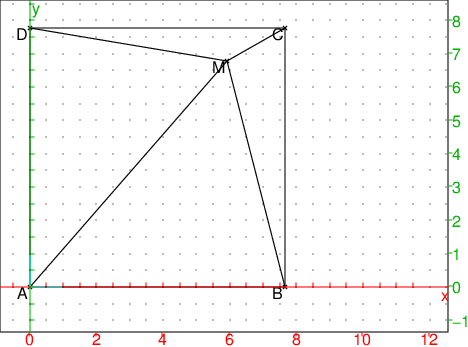
\includegraphics[width=\textwidth]{castrois1}\\
On tape :\\
{\tt longueur(M,A)}\\
On obtient :\\
{\tt 9}\\
On tape :\\
{\tt longueur(M,B)}\\
On obtient :\\
{\tt 7}\\
On tape :\\
{\tt longueur(M,D)}\\
On obtient :\\
{\tt 6}\\
On tape :\\
{\tt longueur(M,C)}\\
On obtient :\\
{\tt 2}\\

Ou bien on utilise $t$ comme param\`etre ($t$ varie entre 0 et 4 pour que 
$y=b^2$ soit positif).
On a $a^2=-36-t,b^2=4-t,c^2=45+t,d^2=t$ donc on tape
\begin{verbatim}
supposons(t=[1,0,4,0.1]);
M:=point(sqrt(36-t),sqrt(45+t));
A:=point(0);
B:=point(sqrt(36-t)+sqrt(4-t));
C:=point(sqrt(36-t)+sqrt(4-t)+i*sqrt(t)+i*sqrt(45+t));
D:=point(i*sqrt(t)+i*sqrt(45+t));
polygone(A,B,C,D);
segment(A,M);
segment(B,M);
segment(C,M);
segment(D,M);
longueur(M,A);
longueur(M,B);
longueur(M,C);
longueur(M,D);
plotparam(affixe(M),t=0..4);
\end{verbatim}
$M$ a comme coordonn\'ees $a,b$.\\
On a $a^2+c^2=81$ et $a^2=(36-t),c^2=(45+t)=-a^2+81$.\\
donc $M$ se trouve sur l'arc $M_0M_1$ du cercle de centre $A$ et 
de rayon 9. avec $M0$ de coordon\'ees $(6,3\sqrt 5)$ et $M1$ de coordonn\'ees 
$(4\sqrt 2,7)$.
%\section{Mesure d'un angle d'un triangle rectangle}

\chapter{G\'eom\'etrie dans l'espace}
\section{Le t\'etra\`edre r\'egulier}\index{tetraedre}\index{sommets}\index{plan}\index{projection}\index{aire}
\subsection{Travail pr\'eparatoire}
Faire d\'ecouper par chaque \'el\`eve dans du papier 4 triangles 
\'equilat\'eraux \'egaux de c\^ot\'e $a=3cm$.\\
 R\'eunir 3 de ces triangles (qu'on nomme $S1AB$, $S2BC$
et $S3CA$) de fa\c{c}on \`a r\'eunir $S1,S2,S3$ en $S$ et d'obtenir une 
pointe de sommet $S$ et de base $ABC$ (les 3 triangles seront reunis selon 
$SA,SB,SC$) :\\
on obtient un t\'etra\`edre dont la face est $ABC$ manquante. Cette face 
manquante peut \^etre combl\'ee par le 4-i\`eme triangle \'equilat\'eral $ABC$. 
Fixer ce 4-i\`eme triangle aux 3 autres et projeter $S$ en $H$ sur cette face 
$ABC$. 
Les questions :\\
\begin{enumerate}
\item O\`u se trouvent $H$ ?
\item Calculer $AH$,$BH$,$CH$,$SH$.
\item Calculer l'angle que font les faces $SAB,SBC,SCA$ avec la face $ABC$.
\item Calculer le volume de ce t\'etra\`edre r\'egulier en fonction de $a=AB$.
\item Ouvrir maintenant la pointe coupant $SA,SB,SC$ pour obtenir une figure 
plane ($S$ va redevenir 3 points $S1,S2,S3$). Qu'obtient-on ?
\item O\`u se trouvent alors les points $A, B, C$ ?
\item Que d\'ecrivent les points $S1,S2,S3$ lorsque l'on replie le triangle 
$S1S2S3$ pour former le t\'etra\`edre $SABC$.
\end{enumerate}

Si $B1$ est la projection de $S3$ sur $AC$, on a :\\
$S3B1=a\sqrt 3/2$, $B1H=a\sqrt 3/6$ et \\
$SH^2=SB1^2-B1H^2=3a^2/4-3a^2/36=2a^2/3$
L'angle $b$ que font les faces entre elles a donc pour tangente :\\
$\tan(b)=SH/B1H=a\sqrt 2/\sqrt 3/(a\sqrt 3/6)=6\sqrt 2/3=2\sqrt 2$
\subsection{V\'erification et calculs avec {\tt Xcas}}\index{milieu}\index{rotation}
On ouvre un niveau de g\'eom\'etrie 3d. On choisit de construire un 
t\'etra\`edre de c\^ot\'e $3$.
 \begin{enumerate}
\item On tape :\\
\begin{verbatim}
A:=point(0,0,0);
B:=point(3,0,0);
C:=point(3/2,sqrt(3)*3/2,0);
T:=tetraedre(A,B,C):;T;
S:=sommets(T)[3];
H:=projection(plan(A,B,C),S);
normal(coordonnees(H))
\end{verbatim}
On obtient pour $H$:\\
{\tt [3/2,(sqrt(3))/2,0]}
\item On tape :\\
{\tt normal(longueur(A,H),longueur(B,H),longueur(C,H))}\\
On obtient :\\
{\tt sqrt(3),sqrt(3),sqrt(3)}\\
On tape :\\
{\tt  normal(longueur(S,H))}\\
On obtient:\\
{\tt sqrt(6)}
\item On tape :\\
{\tt angle(plan(S,A,B),plan(A,B,C))}\\
On obtient :\\
{\tt acos(1/3)}
\item On tape pour avoir le volume du t\'etra\`edre $T$\\
{\tt normal(1/3*longueur(S,H)*aire(triangle(A,B,C)))}\\
On obtient :\\
{\tt 9*sqrt(3)/4}
\item On tape :\\
\begin{verbatim}
A:=point(0,0,0);
B:=point(3,0,0);
C:=point(3/2,sqrt(3)*3/2,0);
T:=tetraedre(A,B,C):;T;
S:=sommets(T)[3];
S1:=rotation(droite(A,B),pi-acos(1/3),S);
S2:=rotation(droite(B,C),pi-acos(1/3),S);
S3:=rotation(droite(C,A),pi-acos(1/3),S);
triangle(S1,S2,S3);
\end{verbatim}
On obtient :\\
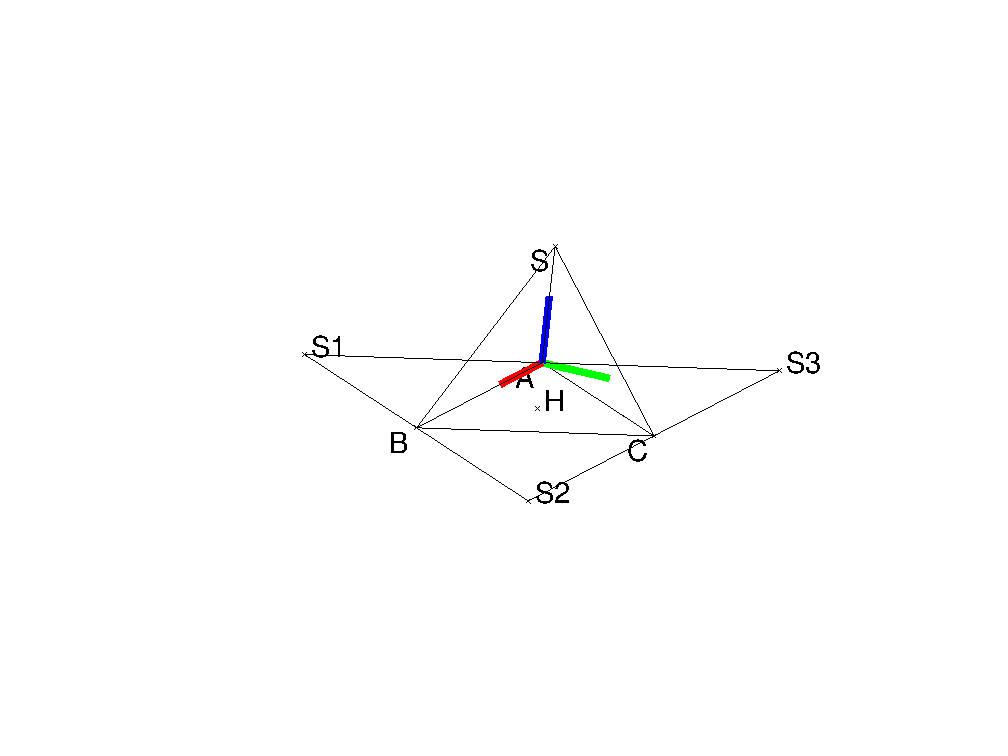
\includegraphics[width=\textwidth]{tetraedre}\\
\item On tape :\\
{\tt normal(coordonnees(milieu(S1,S3))-coordonnees(A))}\\
On obtient :\\
{\tt [0,0,0]}\\
ou on tape :\\
{\tt normal(coordonnees(milieu(S1,S3)))==normal(coordonnees(A))}\\
On obtient :\\
{\tt 1} c'est \`a dire {\tt vrai}\\
On tape :\\
{\tt normal(coordonnees(milieu(S1,S2))-coordonnees(B))}\\
On obtient :\\
{\tt [0,0,0]}\\
On tape :\\
{\tt normal(coordonnees(milieu(S2,S3))-coordonnees(C))}\\
On obtient :\\
{\tt [0,0,0]}
\end{enumerate}
{\bf Remarque}
Si on veut avoir les r\'esultats en fonction de $a$ il faut ajouter le 
param\`etre $a$ avec {\tt Edit} du niveau de g\'eom\'etrie 3d puis
ajouter param\`etre en mettant par exemple que $a$ varie de 0 \`a 5 et en 
mettant $a= 3$ ce qui donne comme niveau 1 :\\
{\tt assume(a=[3,0,5,0.1])} puis on modifie fes d\'efinitions :\\
{\tt B:=point(a,0,0);}\\
{\tt C:=point(a/2,a*sqrt(3)/2,0);} \\
les longueurs sont alors multipli\'ees pas $a/3$ et le volume par $a^3/27$.
\subsection{Faire une animation avec {\tt Xcas}}\index{rotation}\index{milieu}
\index{animation}\index{seq}
Faire une animation qui montre comment en pliant un triangle \'equilat\'eral,
 on obtient un t\'etra\'edre r\'egulier.
On pose $a=6$ et on a $\tan(b)=2\sqrt 2$ donc $b=\atan(2\sqrt 2)\simeq 1.23$
$S1$ subit une rotation d'un angle allant de 0 \`a $\pi-b\simeq 1.91$.\\
On note $MNP$ le triangle $S1S2S3$ et on note $S1$ le transform\'e de $M$ par 
la rotation d'axe $AB$ etc ...\\
Faire attention \`a l'orientation de l'axe de la rotation !!!\\
On tape :\\
\begin{verbatim}
tetreganim(t):={
local S1,S2,S3,A,B,C,c,K,M,N,P;
M:=point(0,0,0):;
N:=point(6,0,0):;
P:=point(3,3*sqrt(3),0):;
triangle(M,N,P);
A:=milieu(M,P);
B:=milieu(M,N);
C:=milieu(N,P);
S1:=rotation(droite(B,A),t,M);
S2:=rotation(droite(C,B),t,N);
S3:=rotation(droite(A,C),t,P);
retourne [affichage(triangle(S1,A,B),1+rempli),
          affichage(triangle(S2,C,B),2+rempli),
          affichage(triangle(S3,A,C),4+rempli)];
}:;
\end{verbatim}
Puis, on tape dans des lignes de commandes (WX-=-3,WX+=7 et les autre-5 et +5):
{\tt L1:=seq([tetreganim(t)],t=0..1.91,0.1):;}\\
{\tt L2:=seq([tetreganim(t)],t=1.91..0,-0.1):;}\\
{\tt animation(L1,L2)}\\
On obtient :\\
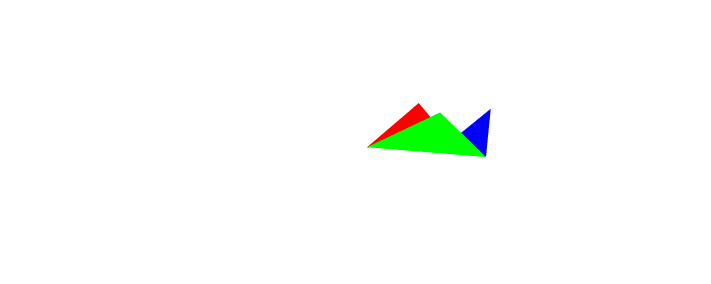
\includegraphics[width=\textwidth]{tetrareg}
\section{Le t\'etra\`edre non r\'egulier ayant 4 faces \'egales}
On veut plier une feuille triangulaire pour en faire un t\'etra\`edre.\\
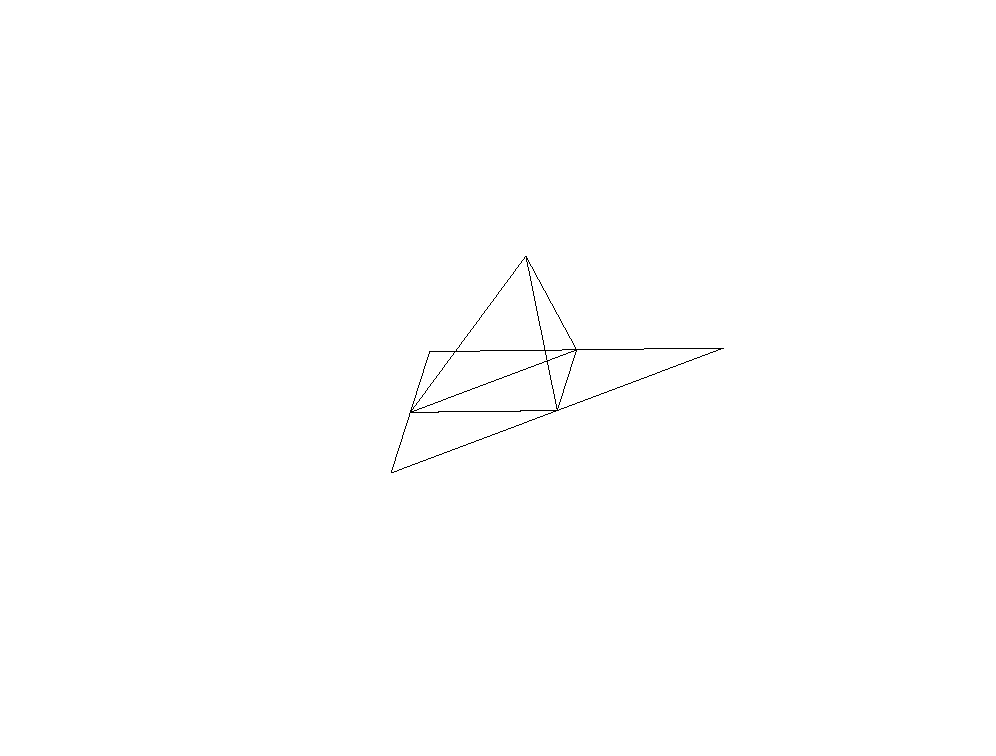
\includegraphics[width=\textwidth]{troisgeo33}\\
Cela est-il toujours possible ?\\
\subsection{Travail pr\'eparatoire}
Soit un triangle $ABC$. On veut le plier pour en faire un t\'etra\`edre $MNPQ$.
On veut plier le triangle $ABC$ pour amener $A,B,C$ en le sommet $Q$.\\
Si cela est possible on aura :\\
$MA=MB=MQ$ si $M$  est le point de pliure sur $AB$,\\
$NB=NC=NQ$ si $N$ est le point de pliure sur $BC$,\\
$PA=PC=PQ$ si $P$ est le point de pliure sur $AC$.\\
Donc le triangle $MNP$ est le triangle qui joint les milieux des c\^ot\'es du 
triangle $ABC$.\\
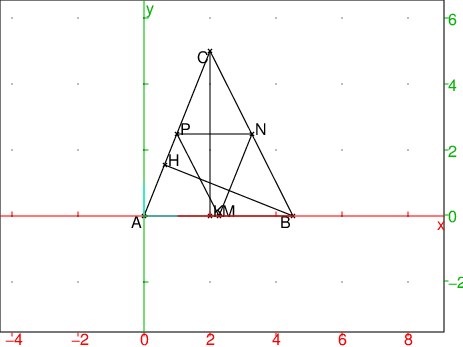
\includegraphics[width=\textwidth]{troisgeo0}\\
Peut-on toujours amener $A,B,C$ en le sommet $Q$ ?\\
Regardons tout d'abord en g\'eom\'etrie plane les propri\'et\'es de la figure 
form\'ee par $ABC$ et $MNP$.\\
Soient $J$ le sym\'etrique de $B$ par rapport \`a $MN$ et $K$ le sym\'etrique de
$C$ par rapport \`a $PN$ (cela revient \`a r\'ealiser les plis $MN$ et $PN$).\\
Montrer que
\begin{itemize}
\item le triangle $MNP$ a ses c\^ot\'es parall\`eles aux c\^ot\'es de $ABC$,
\item $MN=AC/2$, $NP=AB/2$ et $MP=BC/2$,
\item $J$ est le pied de la hauteur de $ABC$ issue de $B$ 
\item $K$ est le pied de la hauteur de $ABC$ issue de $C$ 
\end{itemize}
Regardons maintenant en g\'eom\'etrie dans l'espace o\`u se d\'eplacent les 
points $S2$ et $S3$ ($S2$ (resp $S3$) est le nom de $B$ (resp $C$)) quand on 
fait le pliage.\\
\begin{itemize}
\item Montrer que $S2$ et $S3$ sont sur la sph\`ere de diam\`etre $BC$ (i.e. 
centre $N$ et rayon $BC/2$),
\item Montrer que  $S2$ est aussi sur une 2i\`eme sph\`ere. Laquelle ? 
\item Montrer que  $S3$ est aussi sur une 3i\`eme sph\`ere. Laquelle ? 
\item Lorsque l'on plie selon $MN$, on fait subir au point  $S2$ une 
rotation. Quel est l'axe de cette rotation ? 
\item En d\'eduire que  $S2$ d\'ecrit un cercle de centre le milieu de $BJ$.\\
Ce cercle est l'intersection de 2 sph\`eres lesquelles ?
Montrer que le plan de ce cercle est le plan perpendiculaire en $J$ \`a $AC$.
\item Lorsque l'on plie selon $PN$, on fait subir au point  $S3$ une 
rotation. Quel est l'axe de cette rotation ? 
\item En d\'eduire que  $S2$ d\'ecrit un cercle de centre le milieu de $CK$.\\
Ce cercle est l'intersection de 2 sph\`eres lesquelles ?
Montrer que le plan de ce cercle est le plan perpendiculaire en $K$ \`a $AB$.
\item le probl\`eme sera possible si les cercles que d\'ecrivent $S2$ et $S3$ 
se coupent, c'est \`a dire si les plans de ces 2 cercles se coupent en dehors 
de la sph\`ere  de diam\`etre $BC$. Qu'est-ce que cela signifie pour 
l'orthocentre $H$ du triangle $ABC$ ?
\item Qu'est-ce que cela signifie pour les angles du triangle $ABC$ ?
\end{itemize}


Lorsqu'on plie la feuille selon $MN$, que d\'ecrit le point $B$ ?
Lorsqu'on plie la feuille selon $NP$, que d\'ecrit le point $C$ ?
$C$ d\'ecrit un cercle de diam\`etre $CK$ situ\'e dans le plan perpendiculaire 
\`a $NP$.\\
Ce cercle est la base d'un c\^one d'axe $NP$ et de demi-angle au sommet l'angle
$\widehat{CNP}=\widehat{CBA}$.\\
$B$ d\'ecrit un cercle de diam\`etre $BH$ situ\'e dans le plan perpendiculaire 
\`a $NM$.\\
Ce cercle est la base d'un c\^one d'axe $NM$ et de demi-angle au sommet l'angle
$\widehat{BNM}=\widehat{BCA}$.\\
Ces cercles se coupent-ils ?\\
On a si $BC=a$ et $AC=b$ : $HB=a*\sin(C)$ et $CK=b\sin(A)$\\
Si $\widehat A +\widehat C >\widehat B$ les 2 cercles se coupent.\\
Comme $\widehat A +\widehat C +\widehat B=\pi$ on en d\'eduit que l'on doit 
avoir $\widehat B <\pi/2$\\
de m\^eme on montre que  l'on doit 
avoir $\widehat C <\pi/2$ et $\widehat A <\pi/2$.
Donc le probl\`eme est possible si le triangle de d\'epart n'a que des angles 
aigus.\\
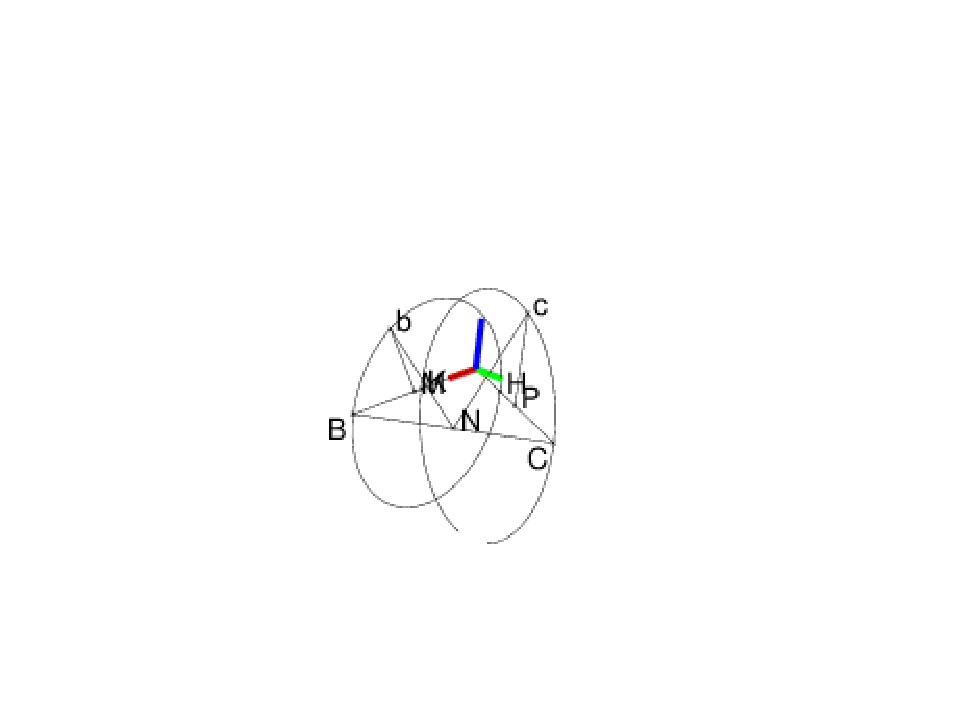
\includegraphics[width=\textwidth]{troisgeo1}

\subsection{Les relations dans un triangle $ABC$}\index{circonscrit}\index{cercle}
Avant de faire une animation, on va rappeler les relations qui relient les 
hauteurs, le rayon $R$ du cercle circonscrit et l'aire $S$ aux 3 cot\'es 
$a,b,c$ du triangle $ABC$.\\
{\bf Rappel}\
Soit un triangle $ABC$.\\
On note $h_a$ (resp $h_b,h_c$) la hauteur issue de $A$ (resp $B,C$),\\
$H$ l'orthocentre de $ABC$\\
$A_1$ le pied de la hauteur issue de $A$\\ 
$A_2$ le milieu de $AA_1$\\
$M$ (res $N,P$) les milieux de $AB$ (resp $BC,AC$)\\
$R$ le rayon du cercle circonscrit\\
$O$ le centre du cercle circonscrit et\\
$S$ l'aire du triangle $ABC$.\\
Si $a$ (resp $b,c$) repr\'esente la longueur du c\^ot\'e $BC$ (resp $AC,AB$),
on pose $\displaystyle p=\frac{a+b+c}{2}$ on a alors :\\
$O$ est l'intersection des m\'ediatrices de $AB$ et $BC$,\\
%(ici point de coordonn\'ees (3.0,1.03571428571)\\
$H$ est le transform\'e de $O$ par l'homoth\'etie de centre $G$ et de 
rapport -2.\\
%(ici point de coordonn\'ees 5.0,1.42857142857)
$\displaystyle S=\sqrt{p(p-a)(p-b)(p-c)}$\\
$\displaystyle R=\frac{abc}{4S}$
$AA_1=h_a=\frac{2S}{a}=\frac{2\sqrt{p(p-a)(p-b)(p-c)}}{a}$\\
$AH=2ON=2\sqrt{R^2-a^2/4}=\sqrt{4R^2-a^2}$\\
$\displaystyle A_2H=AH-\frac{h_a}{2}=\sqrt{4R^2-a^2}-\frac{S}{a}$\\
Si on plie le triangle selon $MP$, $MN$ et $NNP$ afin de reunir les points 
$A,B,C$ en $S$ de fa\c{c}on \`a former le t\'etra\`edre $SMNP$, alors $A$ se 
projette en $H$ orthocentre de $ABC$.\\ 
Si $a_1$ est l'angle de la face $AMP$ avec la face $MNP$ on a  :\\
$\displaystyle \cos(a_1)=2HA_2/AA_1=a*HA_2/S=\frac{a\sqrt{4R^2-a^2}}{S}-1=
\frac{a^2\sqrt{4b^2c^2-4S^2}}{2S^2}-1$\\
De m\^eme si $b_1$ (resp $c1$) est l'angle de la face $BNP$ (resp $CMP$)
avec la face $MNP$ on a  :\\
$\displaystyle \cos(b_1)=\frac{b^2\sqrt{4a^2c^2-4S^2}}{2S^2}-1$\\
$\displaystyle \cos(c_1)=\frac{c^2\sqrt{4a^2b^2-4S^2}}{2S^2}-1$\\
La hauteur du t\'etra\`edre est alors : \\
$\displaystyle h=AA_2\sin(a_1)=\frac{S}{a}\sin(a_1)$\\
Pour faiire une animation on a besoin de connaitre les angles $a_1,b_1,c_1$.\\
On  fait calculer ces angles par {\tt Xcas} avec les formules ci-dessus.\\
On tape :\\
{\tt c:=longueur(A,B);b:=longueur(A,C);a:=longueur(C,B);p:=(a+b+c)/2}\\
On obtient :\\
{\tt 6,6.10327780787,3.64005494464,7.87166637625}\\
On tape :\\
{\tt S:=sqrt(p*(p-a)*(p-b)*(p-c));2*S/c;R:=a*b*c/4/S;sqrt(4*R\verb|^|2-c\verb|^|2)}\\
On obtient :\\
{\tt 10.5,3.5,3.17375236615,2.07142857143}\\
On tape :\\
{\tt a1:=acos(-1+a\verb|^|2*sqrt(c\verb|^|2*b\verb|^|2-4*S\verb|^|2)/(2*S\verb|^|2));pi-a1}\\
On obtient :\\
{\tt 0.638952150388,2.5026405032}\\
On tape :\\
{\tt b1:=acos(-1+b\verb|^|2*sqrt(c\verb|^|2*a\verb|^|2-4*S\verb|^|2)/(2*S\verb|^|2));pi-b1}\\
On obtient :\\
{\tt 1.55719046484,1.58440218875}\\
On tape :\\
{\tt c1:=acos(-1+c\verb|^|2*sqrt(a\verb|^|2*b\verb|^|2-4*S\verb|^|2)/(2*S\verb|^|2));pi-c1}\\
On obtient :\\
{\tt 1.3860741241,1.75551852949}\\
On tape :\\
{\tt h:=S/a*sin(a1)}\\
On obtient :\\
{\tt 1.72022779697}\\
Le sommet du t\'etra\`edre est donc :\\
{\tt Q:= point(5.0,1.42857142857,1.72022779697)}
On tape :\\
{\tt angle(plan(Q,M,P),plan(M,N,P))}\\
On obtient $\pi-a_1$:\\
{\tt 2.5026405032}\\
On tape :\\
{\tt angle(plan(Q,P,M),plan(M,N,P))}\\
On obtient $a_1$:\\
{\tt 0.638952150388}

\subsection{R\'ealisation d'une animation du pliage}
\begin{verbatim}
animtriABC(t):={
local A,B,C,M,N,P,S1,S2,S3;
A:=point(0,0,0):;
B:=point(6,0,0);
C:=point(5,3.5,0);
triangle(A,B,C);
M:=milieu(A,B);
N:=milieu(B,C);
P:=milieu(A,C);
S1:=rotation(droite(M,P),t,A);
S2:=rotation(droite(N,M),t*1.58/2.5,B);
S3:=rotation(droite(P,N),t*1.76/2.5,C);
retourne triangle(M,P,S1),triangle(N,M,S2),triangle(N,P,S3);
}:;
\end{verbatim}
Puis, on tape :
{\tt L1:=seq([animtriABC(t)],t=0..2.5,0.1):;}\\
{\tt L2:=seq([animtriABC(t)],t=2.5..0,-0.1):;}\\
{\tt affichage(Q,1+epaisseur\_point\_2),animation(L1,L2)}\\
On obtient :\\

\includegraphics[width=\textwidth]{troisgeo34}

\chapter{Compl\'ements}
\section{Les calculs avec {\tt Xcas} }
\section{Le tableur de {\tt Xcas}}
On va utiliser le tableur sur un exemple.\\
{\bf L'\'enonc\'e}\\
Au 1ier janvier 2010, $A$ veut emprunter 120000 euros. Les int\'er\^ets de cet 
emprunt ont un taux de 3.8 \% si la dur\'ee du pr\^et est inf\'erieur ou 
\'egale \`a 15 ans et un taux de 4 \% l'an si la dur\'ee du pr\^et est entre 15
et 20 ans.\\ Le remboursement du pret se fait annuellement : 1ier remboursement
1ier janvier 2011, 2nd  remboursement 1ier janvier 2012 etc...).\\
Sachant que $A$ souhaite un remboursement annuel \'egal \`a 9600 euros (soit 800 euros par mois), quel sera dans ce cas le taux de son emprunt et en 
combien de temps le pr\^et sera-t-il rembourser ?\\
Donner le co\^ut de l'emprunt.\\
Trouver par essais-erreurs le montant du remboursement annuel minimum pour 
pouvoir b\'en\'eficier du taux de 3.8\%.\\
Calculer alors le co\^ut de l'emprunt dans ce cas.\\
On ouvre un niveau de tableur (Alt+t) :\\
Dans $A_0$, on tape 120000\\
Dans $B_0$, on tape 0.038\\
Dans $C_0$, on tape 9600\\
Dans $A_1$, on tape $=A_0+A_0*\$B\$0-\$C\$0$\\
puis on recopie cette formule vers le bas on trouve en $A_j$
les sommes \`a rembourser au d\'ebut de la $j$i\`eme ann\'ee.\\
On a  $A_{17}$ =2595.92037452 ce qui veut dire qu'au 1ier janvier 2027 il reste
encore \`a rembourser=2595.92 euros donc  au 1ier janvier 2028 il faudra
 encore rembourser :\\
2595.92037452*1.038=2694.56534875$\simeq$ 2694.57 euros (ou 
encore $A_{18}$ =-6905.43465124 donc au 1ier janvier 2028 il faudra
 encore rembourser 9600-6905.43465124=2694.56534876$\simeq$ 2694.57 euros).\\
Donc le taux applicable dans ce cas est de 4\%. \\
On modifie la valeur de $B_0$ on remplace 0.38 par 0.04.\\
On obtient alors :\\  
$A_{17}$ =6251.94053315 ce qui veut dire qu'au 1ier janvier 2027 (apres 17 
remboursements de 9600 euros) il reste
encore \`a rembourser=6251.94 euros donc au 1ier janvier \`a la fin
 de l'ann\'ee 2028 il faudra encore rembourser 6251.94053315*1.04=6502.01815448$\simeq$ 6502.02 euros (ou 
encore $A_{18}$ =-3097.98184553 donc au 1ier janvier de l'ann\'ee 2028 il faudra
 encore rembourser 9600-3097.98184553=6502.01815447$\simeq$ 6502.02 euros).\\
Le co\^ut de l'emprunt est donc :\\
17*9600+6502.02-120000=49702.02 euros\\
Le banquier offre un taux de 3.8 \% si la dur\'ee du pr\^et est inf\'erieur 
ou \'egale \`a 15 ans.\\
On fait des essais en augmentant le montant du remboursement la valeur de la 
case $A_{15}$ (somme qui reste due au bout de 15 ans i.e apr\`es 15 
remboursements) soit n\'egative.\\
On trouve que pour un remboursement annuel de 10643 euros (soit environ 887 
euros par mois)
$A_{15}$=-9.06558396714.\\
Le montant des int\'er\^ets est donc de :\\
10643*15-9.06558396714-120000=39635.934416$\simeq$ 39635.93 euros
\section{La g\'eom\'etrie 2d de {\tt Xcas}}
\subsection{L'aire d'un secteur circulaire}\index{cercle}
Soit un carr\'e $ABCD$ tel que $AB=1$.\\
On trace l'arc de cercle $BD$ de centre $A$ et de rayon $1$
et l'arc de cercle $AC$ de centre $B$ et de rayon $1$.\\
Ces 2 arcs se coupent en $F$ et d\'eterminent les 4 r\'egions ci-dessous dans 
le carr\'e $ABCD$ :\\
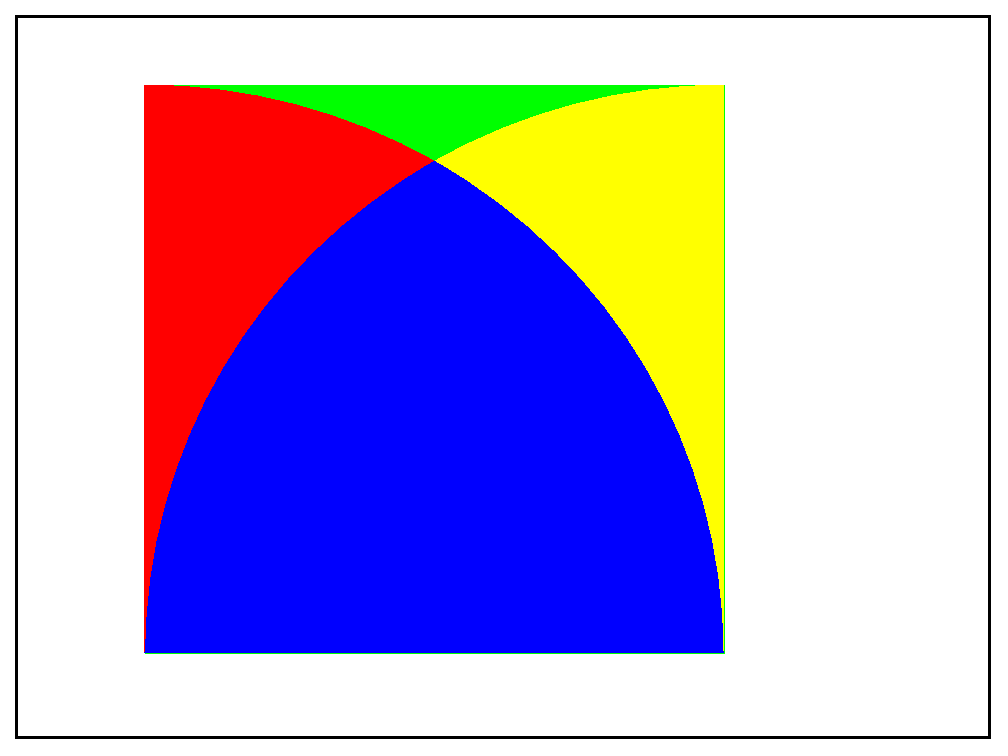
\includegraphics[width=\textwidth]{airearc}\\
Calculer l'aire de chacune de ces r\'egions.\\ 

Pour faire le dessin, on a tap\'e :
\begin{verbatim}
carre(0,1,affichage=vert+rempli);
cercle(0,1,pi/3,pi/2,affichage=1+rempli);
cercle(1,1,pi/2,2*pi/3,affichage=3+rempli);
cercle(0,1,0,pi/3,affichage=4+rempli);
cercle(1,1,2*pi/3,pi,affichage=4+rempli);
\end{verbatim}
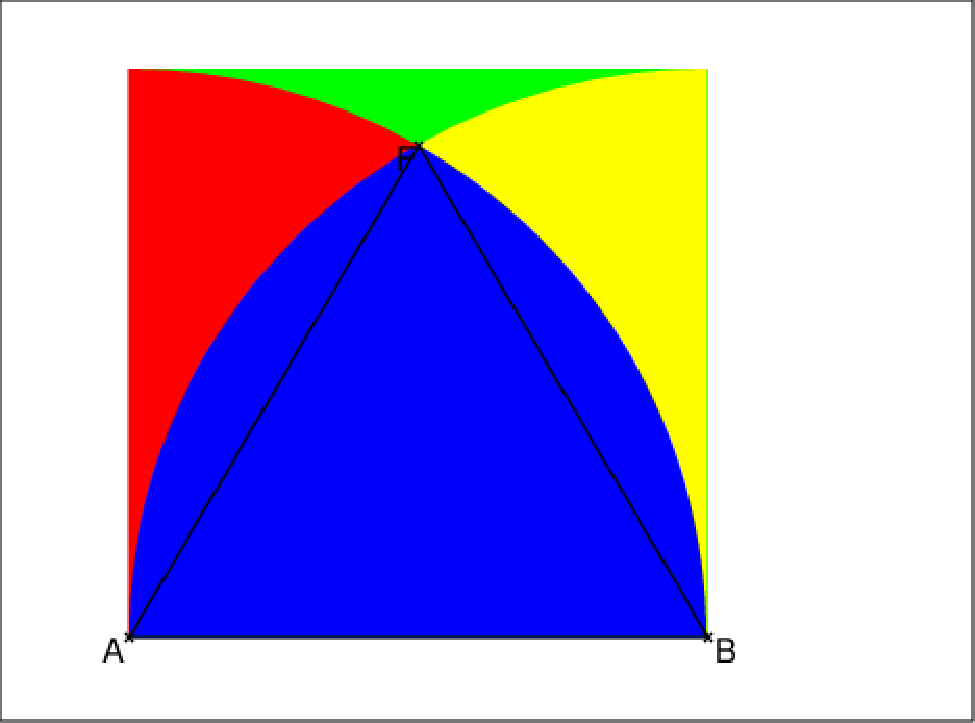
\includegraphics[width=\textwidth]{airearc1}\\
La somme de l'aire bleue et de l'aire du triangle \`equilat\`eral $ABF$ est 
\'egale \`a 2 fois l'aire d'un secteur angulaire d'angle $\pi/3$ et de rayon 1.\\
L'aire d'un secteur angulaire d'angle $\pi/3$ et de rayon 1 est \'egale \`a :\\
$\pi/6$\\
L'aire du triangle \`equilat\`eral $ABF$ est \'egale \`a :\\
$\sqrt 3/4$\\
L'aire bleue est donc \'egale \`a :\\
$2*\pi/6-\sqrt 3/4=\pi/3-\sqrt 3/4$\\
On tape :\\
{\tt evalf(pi/3-sqrt(3)/4)}\\
On obtient l'aire bleue:\\
{\tt 0.614184849304}\\
L'aire rouge est \'egale \`a l'aire jaune et c'est aussi la difference entre 
l'aire du secteur angulaire d'angle $\pi/2$ et de rayon 1 avec l'aire bleue.
L'aire rouge est donc \'egale \`a $\pi/4-\pi/3+\sqrt 3/4=\sqrt 3/4-\pi/12$.\\
On tape :\\
{\tt evalf(-pi/12+sqrt(3)/4)}\\
On obtient l'aire rouge ou l'aire jaune:\\
{\tt 0.171213314093}\\
L'aire verte est \'egale \`a la difference entre l'aire du carr\'e et la somme 
de l'aire rouge de l'aire jaune et de l'aire bleue.\\
L'aire verte est donc \'egale \`a :\\
$1-(-\pi/6+\sqrt 3/2+\pi/3-\sqrt 3/4)=1-\pi/6-\sqrt 3/4$.\\
On tape :\\
{\tt evalf(1-pi/6-sqrt(3)/4)}\\
On obtient l'aire verte:\\
{\tt 0.0433885225095}
\subsection{Le trap\`eze}\index{quadrilatere}
\subsubsection{Longueur du segment joignant les milieux des c\^ot\'es non parall\`eles et aire d'un trap\`eze}\index{}
Soient $ABD$ un trap\`eze : $AB//DC$ ,$AB=a,DC=b$), $M$ le milieu de $AD$, $N$ 
le milieu de $BC$ et les parall\`eles $AB$ et $DC$ sont distantes de $h$.
\begin{itemize}
\item Calculer la longueur du segment $MN$ en fonction de $a$ et $b$.
\item Calculer l'aire du trap\`eze en fonction de $a$ et $b$ et $h$.
\item  Faire un dessin qui montre ces r\'esultats d'un coup d'{\oe}il.
\end{itemize}
On fait les dessins  :\\
la figure 1 est obtenue en tra\c{c}ant un trap\`eze et son sym\'etrique par 
rapport \`a $M$ et on obtient un parall\'elogramme dont 2 c\^ot\'es parall\'eles
sont de longueur $2MN$  distant de $h$,\\
la figure 2  est obtenue en tra\c{c}ant les segments perpendiculaires \`a $AB$ 
passant par $M$ et $N$ et on obtient un rectangle dont les c\^ot\'es ont pour
 longueur $MN$ et $h$ \\
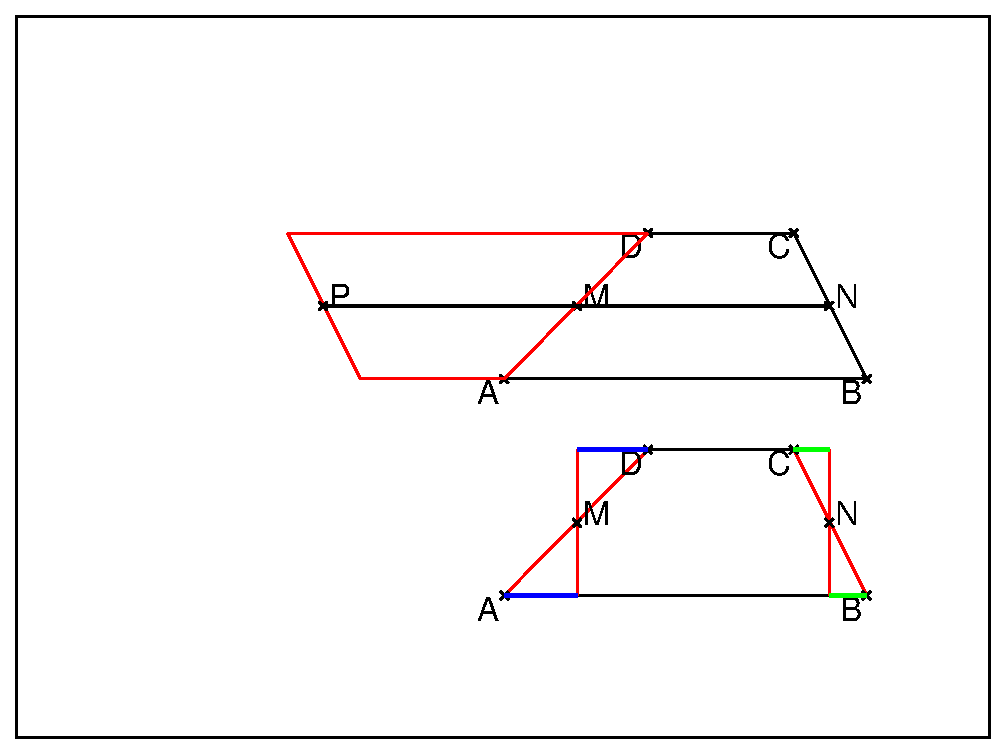
\includegraphics[width=\textwidth]{trapaire}\\
On montre facilement que
$\displaystyle MN=\frac{a+b}{2}$ et que 
l'aire du trap\`eze vaut 
$\displaystyle h(\frac{a+b}{2})$.\\
En effet :\\
la figure 1 est obtenue en tracant un trap\`eze et son sym\'etrique par rapport 
\`a $M$ ce qui forme un parall\'elogramme donc $2MN=a+b$. L'aire du trap\`eze 
est \'egale \`a l'aire du parall\'elogramme et vaut donc $\displaystyle h(\frac{a+b}{2})$.\\
la figure 2 on a $MN=AB-x-y=CD+x+y$ o\`u $x$ (resp $y$) sont les longueurs
 des segments en bleu (resp vert). Donc $2*MN=AB-x-yCD+x+y=AB+CD=a+b$.\\
L'aire du trap\`eze est \'egale \`a l'aire du rectangle et vaut donc
$\displaystyle h(\frac{a+b}{2})$.
\subsubsection{Pavage avec un trap\`eze}
%voir pythagores.xws
Soit un trap\`eze $ABCD$ rectangle en $A$ et v\'erifiant :  $AB=2DC=2AD$.\\
On dira que ce trap\`eze est \`a droite si $(\overrightarrow{AB},\overrightarrow{AD})=+\pi/2$  et qu'il est \`a gauche si $(\overrightarrow{AB},\overrightarrow{AD})=-\pi/2$ 
\begin{itemize}
\item Avec {\tt Xcas}, \'ecrire une fonction {\tt trapd(A,B)} (resp 
{\tt trapg(A,B)}) qui  \'etant 
donn\'e {\tt A} et {\tt B} dessine le trap\`eze  \`a droite (resp \`a gauche)
{\tt ABCD} (on pourra dans un premier temps suppos\'e que le segment $AB$ est
horizontal, dans un deuxi\`eme temps que le segment $AB$ est
horizontal ou vertical et dans un troisi\`eme temps (trop difficile pour la 
classe de troisi\`eme) que le segment $AB$ est quelconque.\\ 
\item Pour faire le dessin avec {\tt Xcas}, en colorant la surface de ces 
trap\`ezes, modifier les fonctions pr\'ec\'edentes en {\tt trapdr(A,B,c)} et
{\tt trapgr(A,B,c)} pour que  \'etant donn\'e {\tt A} et {\tt B} ces fonctions
dessinent le trap\`eze {\tt ABCD} \`a droite et le trap\`eze \`a gauche) dont 
la surface est de couleur {\tt c} (on pourra dans un 
premier temps suppos\'e que le segment $AB$ est horizontal etc...).\\ 
\item Lorsque $ABCD$ est un trap\`eze \`a droite trouver un pavage de 
$ABCD$ par 4 trap\`ezes de m\^eme dimension \`a savoir 3 trap\`ezes rectangles 
\`a droite et 1 trap\`eze rectangle \`a gauche.
\item m\^eme question lorsque $ABCD$ est un trap\`eze \`a gauche.
\item Faire le dessin de ces pavages avec {\tt Xcas} en utilisant 
{\tt trapd(A,B)} et {\tt trapg(A,B)}.
\item Modifier  {\tt trapd(A,B)} (resp {\tt trapg(A,B)}) en supposant que le 
segment $AB$ est horizontal ou vertical.\\
\item La chambre d'un trap\'eziste a la forme d'un rectangle $ABCD$ $AB=4.5m$ 
et $AD=3m$. Il veut paver sa chambre avec 4 trap\`ezes rectangles de couleur 
diff\'erentes (\`a droite ou \`a gauche). Donner lui un ou plusieurs exemple de
pavages. 
\item \'Ecrire une fonction {\tt trapd2(A,B)} et {\tt trapg2(A,B)} qui  \'etant 
donn\'e {\tt A} et {\tt B} ($AB$  horizontal ou vertical) dessine le trap\`eze 
{\tt ABCD} dans lequel les 4 trap\`ezes formant le pavage sont eux aussi 
pav\'es par 4 trap\`ezes.
\item Paver la chambre du trap\'eziste avec 4*4=16 trap\`ezes \`a droite ou \`a
gauche en utilisant trapg2(A,B). Donnerlui un ou plusieurs exemple de pavages. 
\end{itemize}
{\bf La solution}\\
\begin{itemize}
\item On suppose que $AB$ est horizontal, on tape :
\begin{verbatim}
trapd(A,B):={
local a1,a2,b1,b2,D,C;
a1:=abscisse(A);
b1:=abscisse(B);
a2:=ordonnee(A);
b2:=ordonnee(B);
si b2!=a2 alors retourne "AB n'est pas horizontal"; fsi;
D:=point(a1,a2+(b1-a1)/2);
C:=point(a1+(b1-a1)/2,a2+(b1-a1)/2);
retourne quadrilatere(A,B,C,D);
}:;
trapg(A,B):={
local a1,a2,b1,b2,D,C;
a1:=abscisse(A);
b1:=abscisse(B);
a2:=ordonnee(A);
b2:=ordonnee(B);
si b2!=a2 alors retourne "AB n'est pas horizontal"; fsi;
D:=point(a1,a2-(b1-a1)/2);
C:=point(a1+(b1-a1)/2,a2-(b1-a1)/2);
retourne quadrilatere(A,B,C,D);
}:;
\end{verbatim}
On tape :\\
{\tt trapd(0,10),trapg(20,10)}\\
On obtient :\\
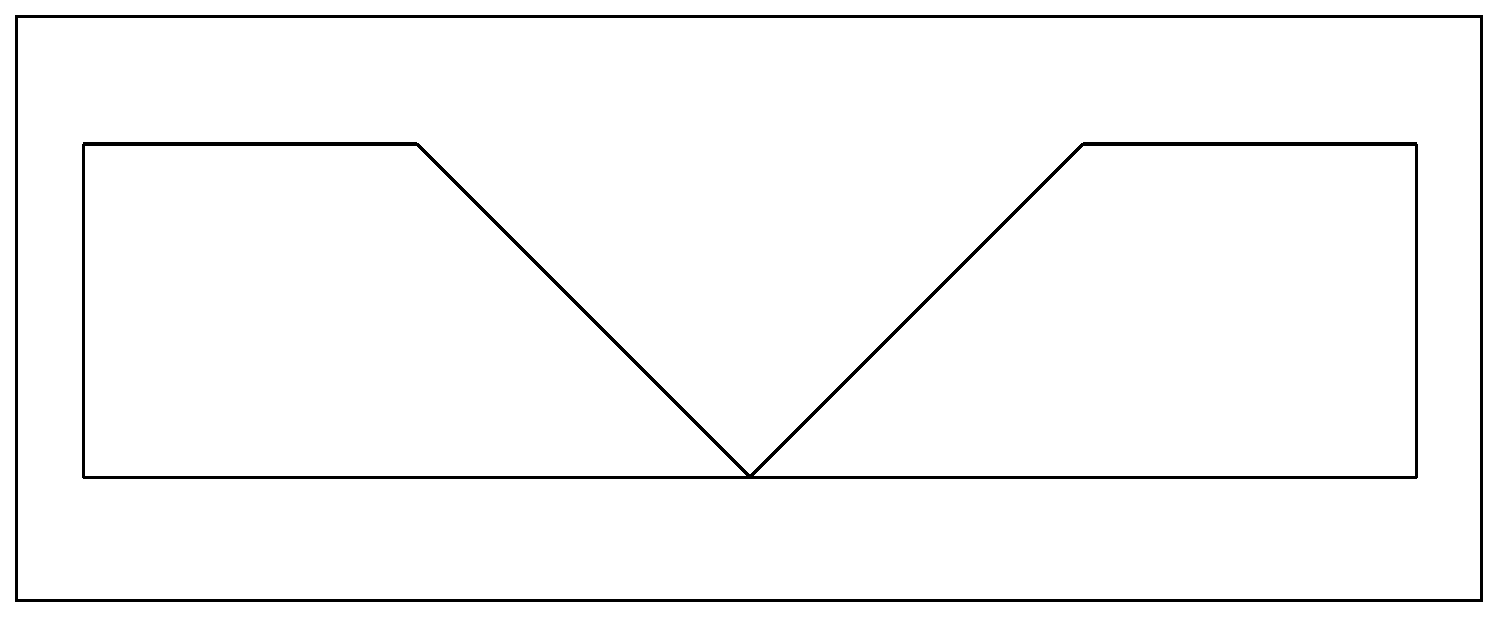
\includegraphics[width=\textwidth]{trapedg}
\item Avec des trap\`ezes remplis avec la couleur  $c$ :
\begin{verbatim}
trapdr(A,B,c):={
local a1,a2,b1,b2,D,C;
a1:=abscisse(A);
b1:=abscisse(B);
a2:=ordonnee(A);
b2:=ordonnee(B);
si b2!=a2 alors retourne "AB n'est pas horizontal"; fsi;
D:=point(a1,a2+(b1-a1)/2);
C:=point(a1+(b1-a1)/2,a2+(b1-a1)/2);
retourne quadrilatere(A,B,C,D,affichage=rempli+c);
}:;
trapgr(A,B,c):={
local a1,a2,b1,b2,D,C;
a1:=abscisse(A);
b1:=abscisse(B);
a2:=ordonnee(A);
b2:=ordonnee(B);
si b2!=a2 alors retourne "AB n'est pas horizontal"; fsi;
D:=point(a1,a2-(b1-a1)/2);
C:=point(a1+(b1-a1)/2,a2-(b1-a1)/2);
retourne quadrilatere(A,B,C,D,affichage=rempli+c);
}:;
\end{verbatim}
On tape :\\
{\tt trapdr(0,10,1),trapgr(20,10,2)}\\
On obtient :\\
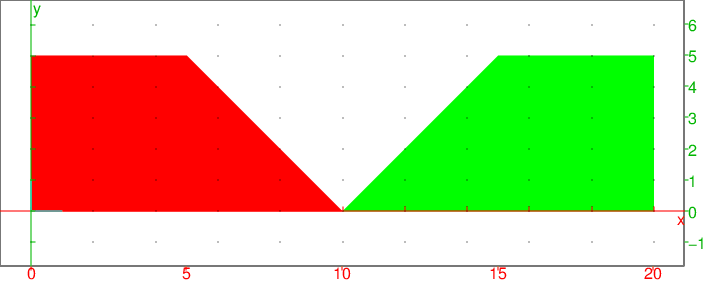
\includegraphics[width=\textwidth]{trapedgr}
\item Le pavage  du trap\`eze droit  (on suppose que $AB$ est horizontal) avec 
4 trap\`ezes non rempli et rempli.\\
On remarquera qu'il est inutile de tracer le trap\`eze pour lequel les bases 
sont verticales.  
\begin{verbatim}
pavaged(A,B):={
local a1,a2,b1,b2,E,F,G,L;
a1:=abscisse(A);
b1:=abscisse(B);
a2:=ordonnee(A);
b2:=ordonnee(B);
si b2!=a2 alors retourne "AB n'est pas horizontal"; fsi;
L:=trapd(A,B);
G:=milieu(A,B);
L:=L,trapd(G,B);
E:=point(a1+(b1-a1)/4,a2+(b1-a1)/4);
F:=point(a1+3*(b1-a1)/4,a2+(b1-a1)/4);
L:=L,trapd(E,F);
L:=L,trapg(G,A);
retourne L;
}:;
pavagedr(A,B,c1,c2,c3,c4):={
local a1,a2,b1,b2,E,F,G,L;
a1:=abscisse(A);
b1:=abscisse(B);
a2:=ordonnee(A);
b2:=ordonnee(B);
si b2!=a2 alors retourne "AB n'est pas horizontal"; fsi;
L:=trapdr(A,B,c1);
G:=milieu(A,B);
L:=L,trapdr(G,B,c2);
E:=point(a1+(b1-a1)/4,a2+(b1-a1)/4);
F:=point(a1+3*(b1-a1)/4,a2+(b1-a1)/4);
L:=L,trapdr(E,F,c3);
L:=L,trapgr(G,A,c4);
retourne L;
}:;
\end{verbatim}
On tape :\\
{\tt pavaged(0,10),pavagedr(point(12),point(25),1,2,3,4)}\\
On obtient :\\
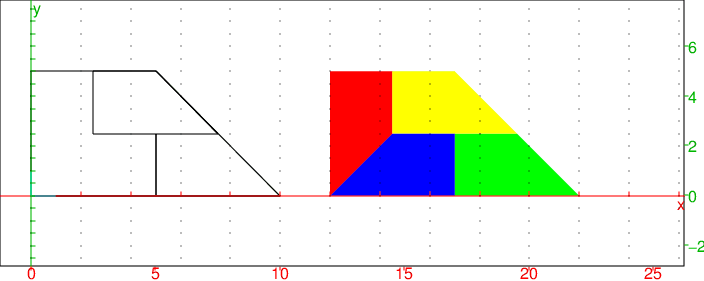
\includegraphics[width=\textwidth]{pavagedr}

\item Le pavage  du trap\`eze gauche (on suppose que $AB$ est horizontal) avec 
4 trap\`ezes non rempli et rempli.\\
On remarquera qu'il est inutile de tracer le trap\`eze pour lequel $AB$ est 
vertical.  
\begin{verbatim}
pavageg(A,B):={
local a1,a2,b1,b2,E,F,G,L;
a1:=abscisse(A);
b1:=abscisse(B);
a2:=ordonnee(A);
b2:=ordonnee(B);
si b2!=a2 alors retourne "AB n'est pas horizontal"; fsi;
L:=trapg(A,B);
L:=L,trapg(milieu(A,B),B);
E:=point(a1+(b1-a1)/4,a2-(b1-a1)/4);
F:=point(a1+3*(b1-a1)/4,a2-(b1-a1)/4);
L:=L,trapg(E,F);
G:=point(a1+(b1-a1)/2,a2)
L:=L,trapd(G,A);
retourne L;
}:;
pavagegr(A,B,c1,c2,c3,c4):={
local a1,a2,b1,b2,E,F,G,L;
a1:=abscisse(A);
b1:=abscisse(B);
a2:=ordonnee(A);
b2:=ordonnee(B);
si b2!=a2 alors 
 retourne "AB n'est pas horizontal"; 
fsi;
L:=trapgr(A,B,c1);
G:=milieu(A,B);
L:=L,trapgr(G,B,c2);
E:=point(a1+(b1-a1)/4,a2-(b1-a1)/4);
F:=point(a1+3*(b1-a1)/4,a2-(b1-a1)/4);
L:=L,trapgr(E,F,c3);
L:=L,trapdr(G,A,c4);
retourne L;
}:;
\end{verbatim}
On tape :\\
{\tt pavageg(10,0),pavagegr(point(22),point(12))}\\
On obtient :\\
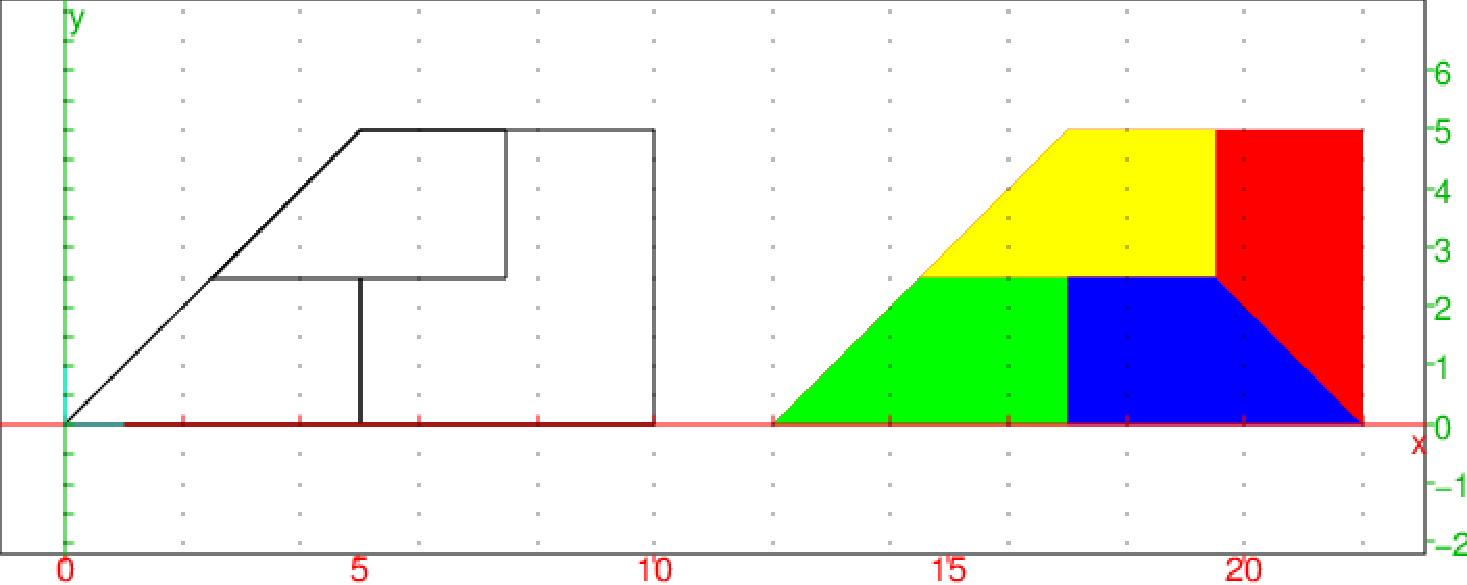
\includegraphics[width=\textwidth]{pavagegr}

\item On suppose que $AB$ est horizontal ou vertical, on tape :
\begin{verbatim}
trapdv(A,B):={
local a1,a2,b1,b2,D,C;
a1:=abscisse(A);
b1:=abscisse(B);
a2:=ordonnee(A);
b2:=ordonnee(B);
si (a1!=b1 et b2!=a2) alors 
 retourne "AB n'est ni horizontal ni vertical"; 
fsi;
si (a2==b2) alors 
  D:=point(a1,a2+(b1-a1)/2);
  C:=point(a1+(b1-a1)/2,a2+(b1-a1)/2);
sinon
  D:=point(a1-(b2-a2)/2,a2);
  C:=point(a1-(b2-a2)/2,a2+(b2-a2)/2);
fsi
retourne quadrilatere(A,B,C,D);
}:;
trapdvr(A,B,coul):={
local a1,a2,b1,b2,D,C;
a1:=abscisse(A);
b1:=abscisse(B);
a2:=ordonnee(A);
b2:=ordonnee(B);
si (a1!=b1 et b2!=a2) alors
  retourne "AB n'est ni horizontal ni vertical"; 
fsi;
si (a2==b2) alors 
  D:=point(a1,a2+(b1-a1)/2);
  C:=point(a1+(b1-a1)/2,a2+(b1-a1)/2);
sinon
  D:=point(a1-(b2-a2)/2,a2);
  C:=point(a1-(b2-a2)/2,a2+(b2-a2)/2);
fsi
retourne quadrilatere(A,B,C,D,affichage=rempli+coul);
}:;
trapgv(A,B):={
local a1,a2,b1,b2,D,C;
a1:=abscisse(A);
b1:=abscisse(B);
a2:=ordonnee(A);
b2:=ordonnee(B);
si (a1!=b1 et b2!=a2) alors 
  retourne "AB n'est ni horizontal ni vertical";
fsi;
si (a2==b2) alors 
  D:=point(a1,a2-(b1-a1)/2);
  C:=point(a1+(b1-a1)/2,a2-(b1-a1)/2);
sinon
  D:=point(a1+(b2-a2)/2,a2);
  C:=point(a1+(b2-a2)/2,a2+(b2-a2)/2);
fsi
retourne quadrilatere(A,B,C,D);
}:;
trapgvr(A,B,coul):={
local a1,a2,b1,b2,D,C;
a1:=abscisse(A);
b1:=abscisse(B);
a2:=ordonnee(A);
b2:=ordonnee(B);
si (a1!=b1 et b2!=a2) alors 
  retourne "AB n'est ni horizontal ni vertical"; 
fsi;
si (a2==b2) alors 
  D:=point(a1,a2-(b1-a1)/2);
  C:=point(a1+(b1-a1)/2,a2-(b1-a1)/2);
sinon
  D:=point(a1+(b2-a2)/2,a2);
  C:=point(a1+(b2-a2)/2,a2+(b2-a2)/2);
fsi
retourne quadrilatere(A,B,C,D,affichage=rempli+coul);
}:;
\end{verbatim}
\item On peut r\'e\'ecrire les fonctions pavages lorsqu'on suppose $AB$ 
horizontal ou vertical.\\
On tape pour avoir le pavage droit avec 4 trap\`ezes rempli avec les couleurs 
$c1,c2,c3,c4$ :
\begin{verbatim}
pavagedvr(A,B,c1,c2,c3,c4):={
local a1,a2,b1,b2,E,F,G,L;
a1:=abscisse(A);
b1:=abscisse(B);
a2:=ordonnee(A);
b2:=ordonnee(B);
si (b2!=a2 et a1!=b1) alors 
  retourne "AB n'est ni horizontal ni vertical"; 
fsi;
G:=milieu(A,B);
L:=trapdvr(G,B,c2);
L:=L,trapgvr(G,A,c4);
si (a2==b2) alors 
  L:=L,trapdvr(point(a1,a2+(b1-a1)/2),A,c1);
  E:=point(a1+(b1-a1)/4,a2+(b1-a1)/4);
  F:=point(a1+3*(b1-a1)/4,a2+(b1-a1)/4);
  L:=L,trapdvr(E,F,c3);
sinon 
  L:=L,trapdvr(point(a1-(b2-a2)/2,a2),A,c1);
  E:=point(a1-(b2-a2)/4,a2+(b2-a2)/4);
  F:=point(a1-(b2-a2)/4,a2+3*(b2-a2)/4);
  L:=L,trapdvr(E,F,c3);
fsi;
retourne L;
}:;
\end{verbatim}
On tape pour avoir le pavage droit avec 4 trap\`ezes rempli avec les couleurs 
$c1,c2,c3,c4$ :
\begin{verbatim}
pavagegvr(A,B,c1,c2,c3,c4):={
local a1,a2,b1,b2,E,F,G,L;
a1:=abscisse(A);
b1:=abscisse(B);
a2:=ordonnee(A);
b2:=ordonnee(B);
si (b2!=a2 et a1!=b1) alors 
  retourne "AB n'est ni horizontal ni vertical"; 
fsi;
G:=milieu(A,B);
L:=trapgvr(G,B,c2);
L:=L,trapdvr(G,A,c4);
si (a2==b2) alors 
  L:=L,trapgvr(point(a1,(a1-b1)/2),A,c1);
  E:=point(a1+(b1-a1)/4,a2-(b1-a1)/4);
  F:=point(a1+3*(b1-a1)/4,a2-(b1-a1)/4);
  L:=L,trapgvr(E,F,c3);
sinon 
  L:=L,trapgvr(point(a1+(b2-a2)/2,a2),A,c1);
  E:=point(a1+(b2-a2)/4,a2+(b2-a2)/4);
  F:=point(a1+(b2-a2)/4,a2+3*(b2-a2)/4);
  L:=L,trapgvr(E,F,c3);
fsi;
retourne L;
}:;
\end{verbatim}
On tape :\\
{\tt pavagedvr(0,10*i,1,2,3,4),pavagegvr(2,2+10i,1,2,3,4)}\\
On obtient :\\
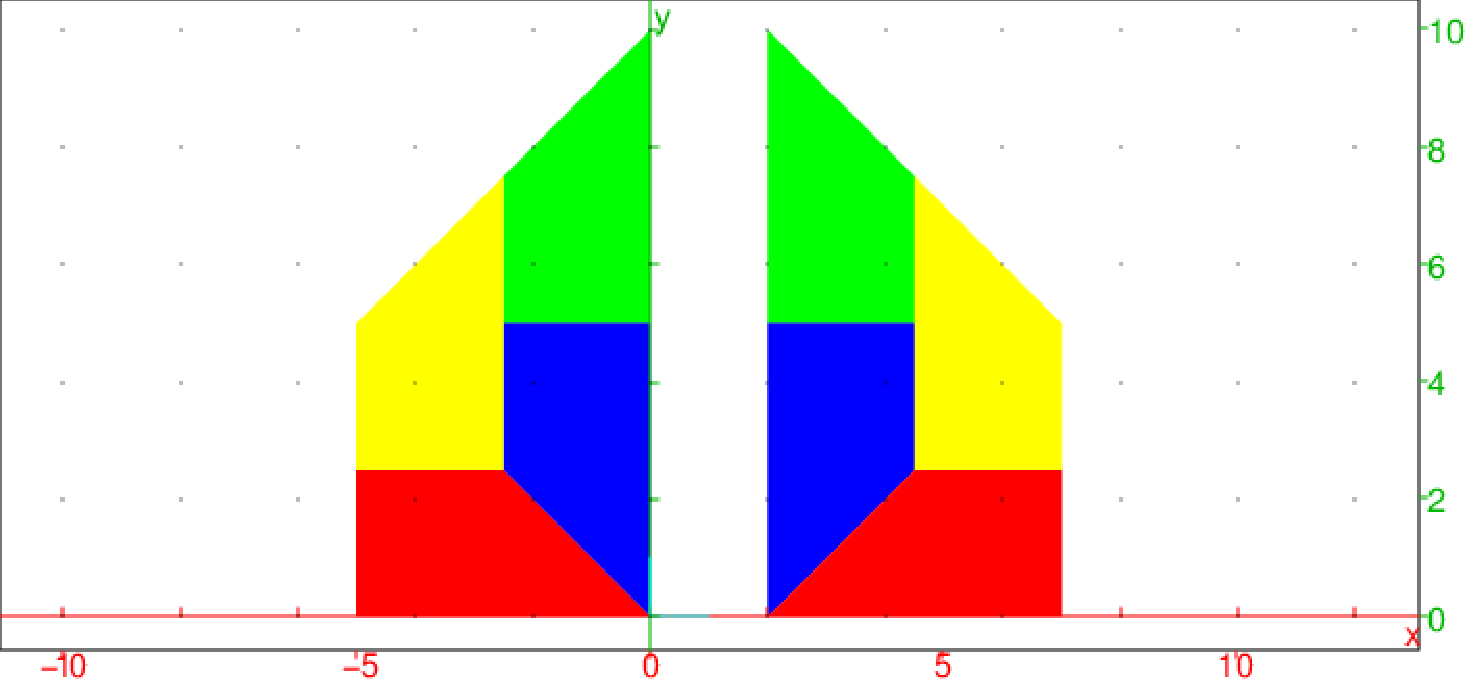
\includegraphics[width=\textwidth]{pavagedgv}

\item
\begin{verbatim}
trapezist4(c1,c2,c3,c4):={
local L;
L:=trapgvr(3,0,c1);
L:=L,trapdvr(3*i,0,c2);
L:=L,trapdvr(4.5,4.5+3*i,c3);
L:=L,trapgvr(1.5+3*i,4.5+3*i,c4);
retourne L;
}:;
\end{verbatim}
On tape :\\
{\tt trapezist4(1,2,3,4)}\\
On obtient :\\

\includegraphics[width=\textwidth]{trapezist4}\\
une autre possibilit\'e :
\begin{verbatim}
trapeziste4(c1,c2,c3,c4):={
local L;
L:=trapdvr(0,3,c1);
L:=L,trapdvr(4.5+1.5*i,1.5+1.5*i,c2);
L:=L,trapgvr(3*i,3+3*i,c3);
L:=L,trapgvr(4.5+1.5*i,1.5+1.5*i,c4);
retourne L;
}:;
\end{verbatim}
On tape :\\
{\tt trapeziste4(1,2,3,4)}\\
On obtient :\\

\includegraphics[width=\textwidth]{trapesiste4}
\item Pavage avec 16 trap\`ezes
\begin{verbatim}
trapezist16(c1,c2,c3,c4):={
local L;
L:=pavagegvr(3,0,c2,c3,c1,c4);
L:=L,pavagedvr(3*i,0,c4,c1,c2,c3);
L:=L,pavagedvr(4.5,4.5+3*i,c1,c4,c3,c2);
L:=L,pavagegvr(1.5+3*i,4.5+3*i,c3,c2,c4,c1);
retourne L;
}:;
\end{verbatim}
On tape :\\
{\tt trapezist16(1,2,3,4)}\\
On obtient :\\
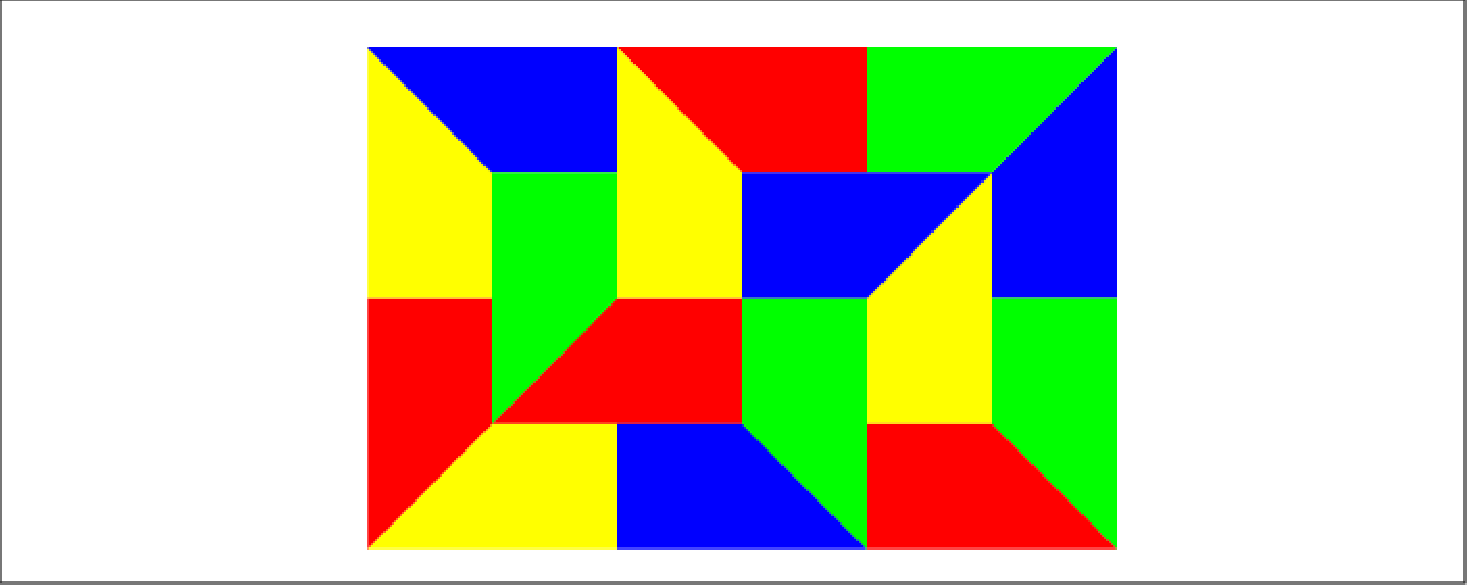
\includegraphics[width=\textwidth]{trapeze16}
\item Un exemple de pavage d'un carr\'e avec 24 trap\`ezes
\begin{verbatim}
tapis(c1,c2,c3,c4):={
local L;
L:=pavagedvr(0,3,c1,c2,c3,c4);
L:=L,pavagedvr(4.5,4.5+3*i,c1,c2,c3,c4);
L:=L,pavagedvr(4.5+4.5*i,1.5+4.5*i,c1,c2,c3,c4);
L:=L,pavagedvr(4.5*i,1.5*i,c1,c2,c3,c4);
L:=L,trapgvr(2.25+2.25*i,3.75+2.25*i,c1);
L:=L,trapgvr(2.25+2.25*i,2.25+3.75*i,c2);
L:=L,trapgvr(2.25+2.25*i,0.75+2.25*i,c1);
L:=L,trapgvr(2.25+2.25*i,2.25+0.75*i,c2);
L:=L,trapgvr(3+1.5*i,3,c4),trapgvr(3+3*i,4.5+3*i,c4);
L:=L,trapgvr(1.5+3*i,1.5+4.5*i,c4);
L:=L,trapgvr(1.5+1.5*i,1.5*i,c4);
return L;
}:;
\end{verbatim}
On tape :\\
{\tt tapis(1,2,3,4)}\\
On obtient :\\
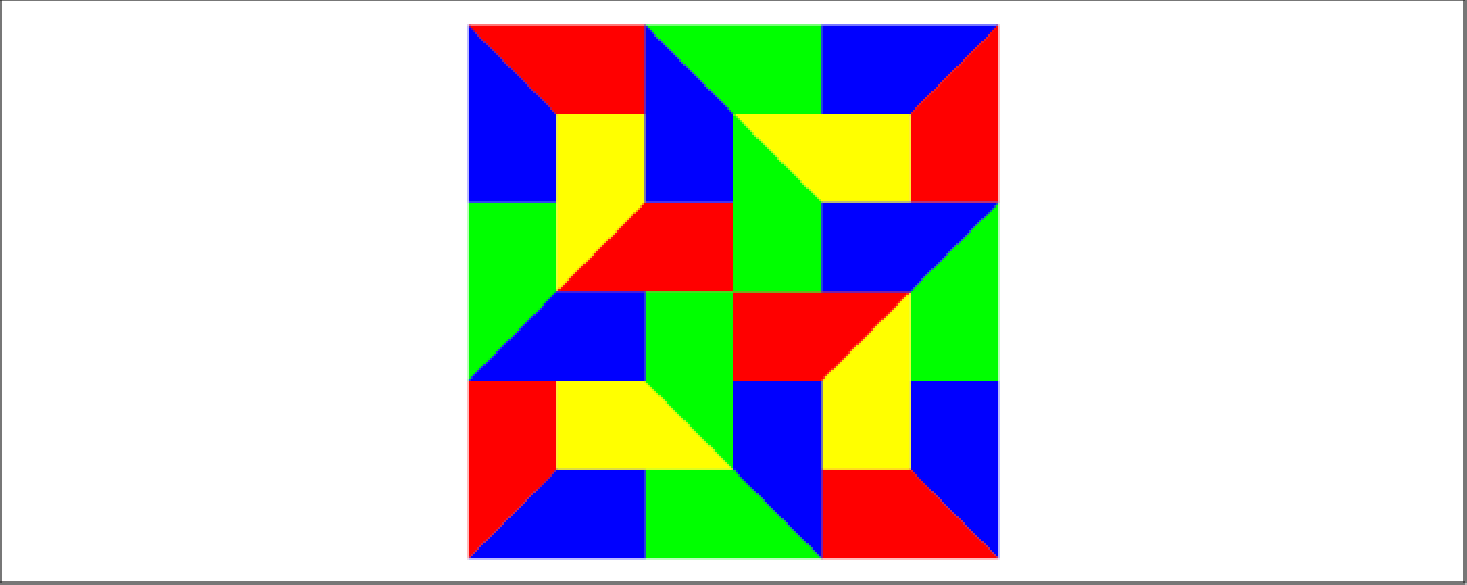
\includegraphics[width=\textwidth]{traptapis}
On tape :\\
{\tt tapis(161,172,183,194)}\\
On obtient :\\
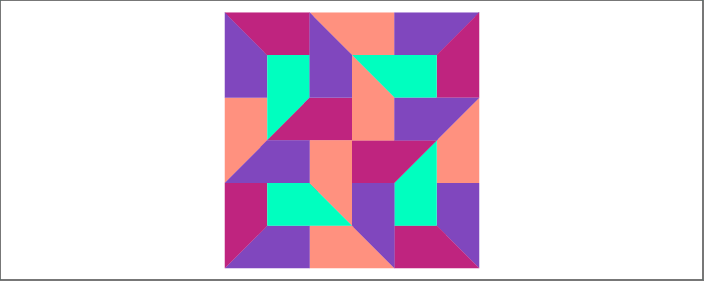
\includegraphics[width=\textwidth]{trapetap}
\end{itemize}

\subsection{Le bassin et la piscine}
{\bf Les Bassins}
%bassin.xws
Voici 4  bassins $B-0,B_1,B_2,B_3$. Ils sont form\'es par un arc de cercle de 
rayon $r$ et d'angle au centre $a_0=2\pi$, $a_1=5\pi/3$, $a_2=3\pi/2$, 
$a_3=4\pi/3$ et on ferme les 3 derniers  par un segment :\\
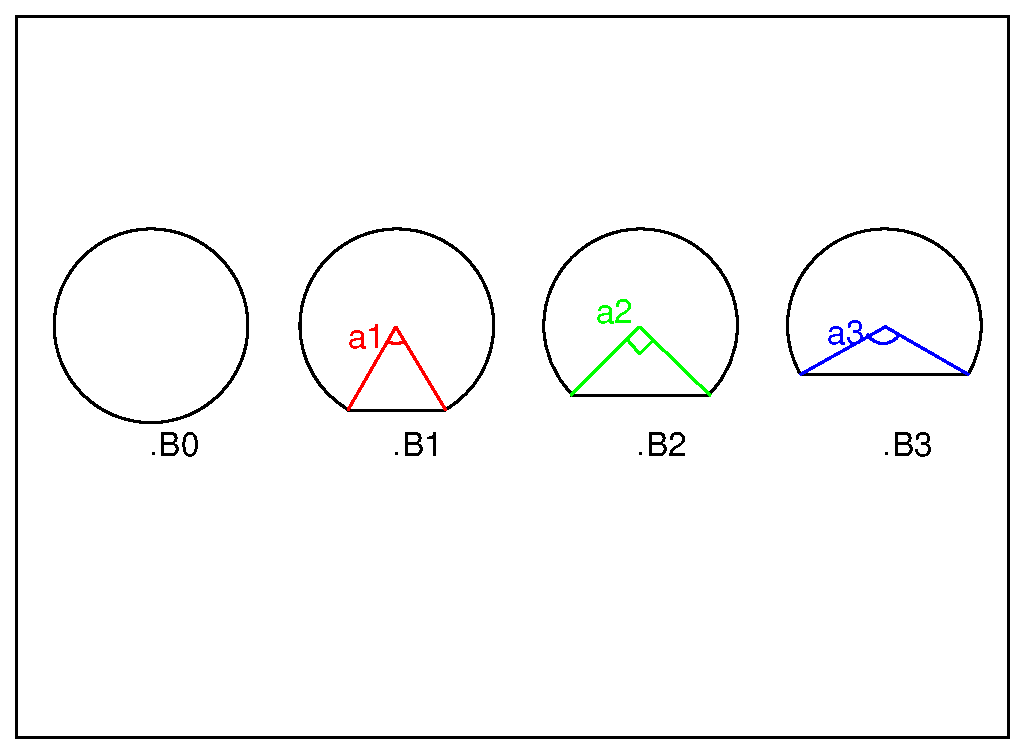
\includegraphics[width=\textwidth]{bassin}\\
Calculer les aires $S_k$ de 4 bassins $B_k$ ($k=1,2,3$) en fonction de $r$.\\
Sur une bande de terre de largeur $a$, on veut implanter l'un de ces bassins
(cf la figure ci-dessous).\\
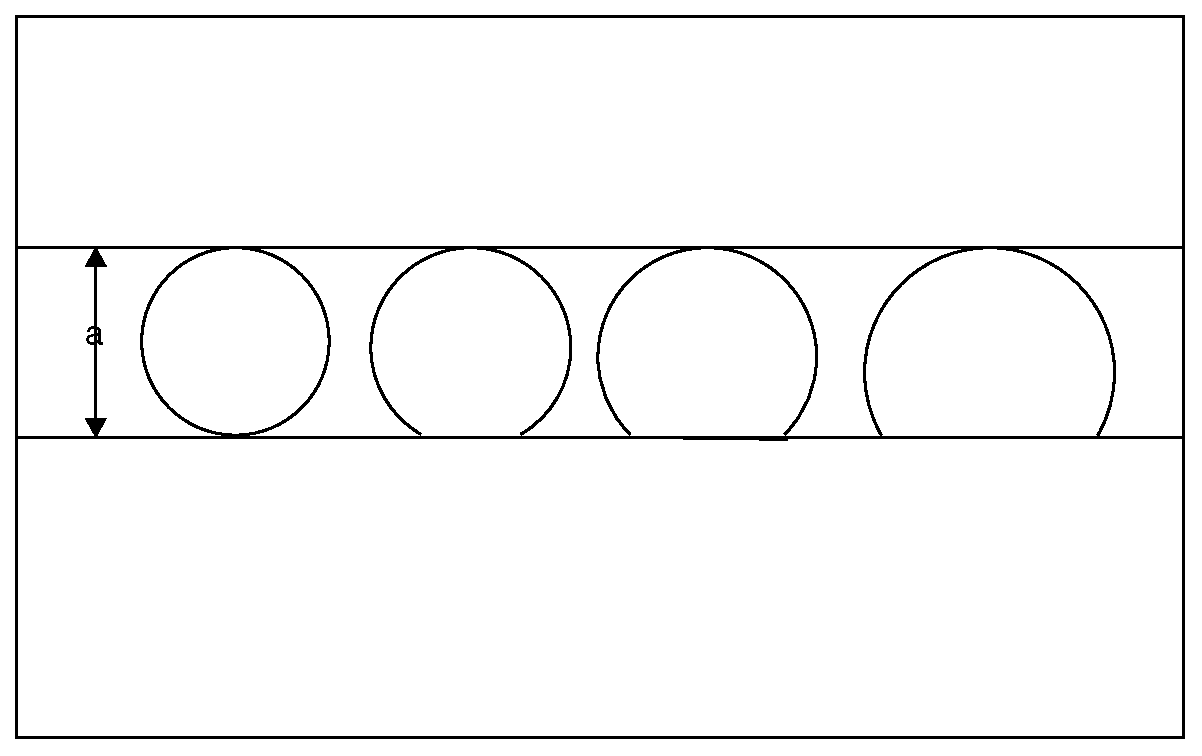
\includegraphics[width=\textwidth]{bassin1}\\
Calculer pour chaque bassin la valeur de $r$ en fonction de $a$.
Calculer en fonction de $a$ les aires $A_k$ de 4 bassins $B_k$ ($k=1,2,3$).\\
0n suppose maintenant que $a=3$. \\
Quel est alors le bassin qui a la plus grande surface ?\\
Montrer que $B_3$ est inscrit dans un rectangle de largeur 3 et de longueur 4.
On coupe alors les bassins $Bk$ ($k=0,1,2,3$) selon leur axe de sym\'etrie et 
on accole chacune des ces moiti\'es \`a un rectangle de fa\c{c}on \`a ce que 
chaque bassin soit inscrit dans un rectangle de largeur 3 et de longueur 4.\\
Calculer alors l'aire de ces nouveaux bassins $C_k$ ($k=0,1,2,3$)\\
Quel est alors le bassin $C_k$ ($k=0,1,2,3$) qui a la plus grande surface ?\\

{\bf Calcul \`a la main}\\
Pour calculer les aires des bassins, il faut connaitre l'aire d'un secteur
angulaire et l'aire d'un triangle.\\
L'aire d'un triangle equilat\'eral de c\^ot\'e $r$ est $\sqrt 3 r^2/4$.\\
L'aire d'un triangle rectangle isoc\`ele de c\^ot\'es $r,r,r\sqrt 2$ est 
$r^2/2$.\\
L'aire d'un triangle isoc\`ele d'angle $2\pi/3,\pi/6,\pi/6$, de c\^ot\'es 
$r,r,r\sqrt 3$ est $\sqrt 3 r^2/4$.\\
On a :\\
$S_0=\pi r^2$\\
$S_1=5\pi r^2/6+\sqrt 3 r^2/4$\\
$S_2=3\pi r^2/4+r^2/2$\\
$S_3=2\pi r^2/3+\sqrt 3 r^2/4$\\

Pour calculer les rayons des bassins implant\'es sur une bande de terre de 
largeur $a$, on doit r\'esoudre les \'equations :\\
$a=2*r_0$ donc $r_0=a/2$\\
$a=r_1+r_1\sqrt 3/2$ donc $r_1=2a/(2+\sqrt 3)=2a(2-\sqrt 3)$\\
$a=r_2+r_2\sqrt 2/2$ donc $r_2=2a/(2+\sqrt 2)=a(2-\sqrt 2)$\\
$a=r_3+r_3/2$ donc $r_3=2a/3$\\
Les aires $A_k$ ($k=1,2,3$) des diff\'erents bassins sont donc :\\
$A_0(a)=\pi a^2/4$
$A_1(a)=5\pi r_1^2/6+\sqrt 3 r_1^2/4=4a^2(2-\sqrt 3)^2(5\pi/6+\sqrt 3/4)=a^2(7-4\sqrt 3)(10\pi/3+\sqrt 3) $\\
$A_2(a)=3\pi r_2^2/4+r_2^2/2=a^2(2-\sqrt 2)^2(3\pi/4+1/2)=(3\pi/2+1) a^2(3-\sqrt 2)$\\
$A_3(a)=2\pi r_3^2/3+\sqrt 3 r_3^2/4=4a^2/9(2\pi /3+\sqrt 3/4)=a^2(8\pi /27+\sqrt 3/9)$\\
Puis, on fait un calcul approch\'e avec {\tt Xcas}.

{\bf Calcul avec {\tt Xcas}}\\
Pour le bassin $B_0$ son aire $S_0=\pi r^2$/
Pour les bassins $B_k$ ($k=1,2,3$), on cherche les coordonn\'ees des segments 
$A_kB_k$ qui ferment les bassins $B_k$.\\
Avec {\tt Xcas}, on tape pour faire le dessin :\\
{\tt assume(r=[1,-5,5,0.1])}\\
{\tt B0:=cercle(point(-5,0),r)}\\
{\tt B1:=cercle(-5/2,r,-pi/3,4*pi/3),
segment(-5/2+r*(-1/2-i*sqrt(3)/2),-5/2+r*(1/2-i*sqrt(3)/2))}\\
{\tt B2:=cercle(0,r,-pi/4,5*pi/4),
segment(r*(-sqrt(2)/2*(1+i)),r*(sqrt(2)/2*(1-i)))}\\
{\tt B3:=cercle(5/2,r,-pi/6,7*pi/6),
segment(5/2+r*(-sqrt(3)/2-i/2),5/2+r*(sqrt(3)/2-i/2))}\\
Pour calculer les aires, on tape :\\
{\tt S0:=aire(cercle(point(-5,0),r))}\\
On obtient :\\
{\tt pi*r\verb|^|2}\\
On tape :\\
{\tt S1:=aire(cercle(-5/2,r,-pi/3,4*pi/3))+aire(triangle(
 -5/2,-5/2+r*(-1/2-i*sqrt(3)/2),-5/2+r*(1/2-i*sqrt(3)/2)))}\\
On obtient :\\
{\tt 5*pi*r\verb|^|2/6+(sqrt(3))/4*r\verb|^|2}\\
On tape :\\
{\tt S2:=aire(cercle(0,1,-pi/4,5*pi/4))+aire(triangle(
0,r*(-sqrt(2)/2*(1+i)),r*(sqrt(2)/2*(1-i))))}\\
On obtient :\\
{\tt 3*pi*r\verb|^|2/4+1/2*r\verb|^|2}\\
On tape :\\
{\tt S3:=aire(cercle(5/2,r,-pi/6,7*pi/6))+aire(triangle(
5/2,5/2+r*(-sqrt(3)/2-i/2),5/2+r*(sqrt(3)/2-i/2)))}\\
On obtient :\\
{\tt 2*pi*r\verb|^|2/3+(sqrt(3))/4*r\verb|^|2}\\

Calcul des diff\'erents rayons.\\
On tape :\\
{\tt r0:=normal(solve(a=2*r,r))}\\
On obtient :\\
{\tt a/2}\\
On tape :\\
{\tt r1:=op(normal(solve(a=r+r*sqrt(3)/2,r)))}\\
On obtient :\\
{\tt (-2*sqrt(3)+4)*a}\\
On tape :\\
{\tt r2:=op(normal(solve(a=r+r*sqrt(2)/2,r)))}\\
On obtient :\\
{\tt (-(sqrt(2))+2)*a}\\
On tape :\\
{\tt r3:=op(normal(solve(a=r+r/2,r)))}\\
On obtient :\\
{\tt 2*a/3}\\
On tape :\\
{\tt A0:=evalf(subst(S0,r=r0))*a\verb|^|2}\\
On obtient :\\
{\tt 0.785398163397*a\verb|^|2}\\
On tape :\\
{\tt A1:=evalf(subst(S1,r=r1))*a\verb|^|2}\\
On obtient :\\
{\tt 0.876209667375*a\verb|^|2}\\
On tape :\\
{\tt evalf(subst(S2,r=r2))*a\verb|^|2}\\
On obtient :\\
{\tt A2:=0.980091001933*a\verb|^|2}\\
On tape :\\
{\tt A3:=evalf(factoriser(subst(S3,r=r3))*a\verb|^|2}\\
On obtient :\\
{\tt 1.12329235746*a\verb|^|2}\\
Donc :\\
$A_0\simeq 0.785398163397a^2$\\
$A_1\simeq 0.876209667375a^2$\\
$A_2\simeq 0.980091001933a^2$\\
$A_3\simeq 1.12329235746a^2$\\
Si $a=3$ on a alors :\\
$A_0\simeq 7.06858347057$\\
$A_1\simeq 7.88588700637$\\
$A_2\simeq 8.8208190174$\\
$A_3\simeq 10.1096312171$\\
Le bassin $C_0$ est constitu\'e de 2 demi-cercles de rayon 3/2 et d'un 
rectangle de c\^ot\'es 1 et 3.\\
Donc son aire vaut :\\
 $9\pi/4+3 \simeq A_0+3 \simeq 10.0685834706$\\
Le bassin $C_1$ est constitu\'e de 2 demi-cercles de rayon 
$r_1=6(2-\sqrt 3)\simeq 1.60769515459$ et d'un 
rectangle de c\^ot\'es $4-2r_1\simeq 0.784609690826$ et 3.\\
Donc son aire vaut :\\
 $(5*pi/6+\sqrt 3/4)*r1^2+3*(4-2*r1)\simeq A_1+3*0.784609690826\simeq 10.2397160788$\\
Le bassin $C_2$ est constitu\'e de 2 demi-cercles de rayon :
$r_2=3(2-\sqrt 2)\simeq 1.75735931288$ et d'un 
rectangle de c\^ot\'es $4-2r_2\simeq 0.485281374239$ et 3.
Donc son aire vaut :\\
$3\pi r_2^2/4+r_2^2/2+3(4-2r_2)\simeq A_2+3*0.485281374239\simeq 10.2766631401$\\
Le bassin $C_3$ est le m\^eme que $B_3$
Donc son aire vaut : $2\pi/3*2^2+\sqrt 3 \simeq 10.1096312171$\\
Dans ce cas le bassin le plus grand est $C_2$\\

{\bf La piscine}
Monsieur X veut faire une piscine s'inscrivant dans un rectangle de largeur
$2$unit\'es et de longueur $6$unit\'es mais il veut que les 2 bords les plus 
petits soient arrondis.
On lui propose les 4 solutions $P_k$ ($k=0,1,2,3$) suivantes : 
on coupe chaque bassin $Bk$ ($k=0,1,2,3$) selon son axe de sym\'etrie et on 
accole chacune des ces moiti\'es \`a un rectangle :\\
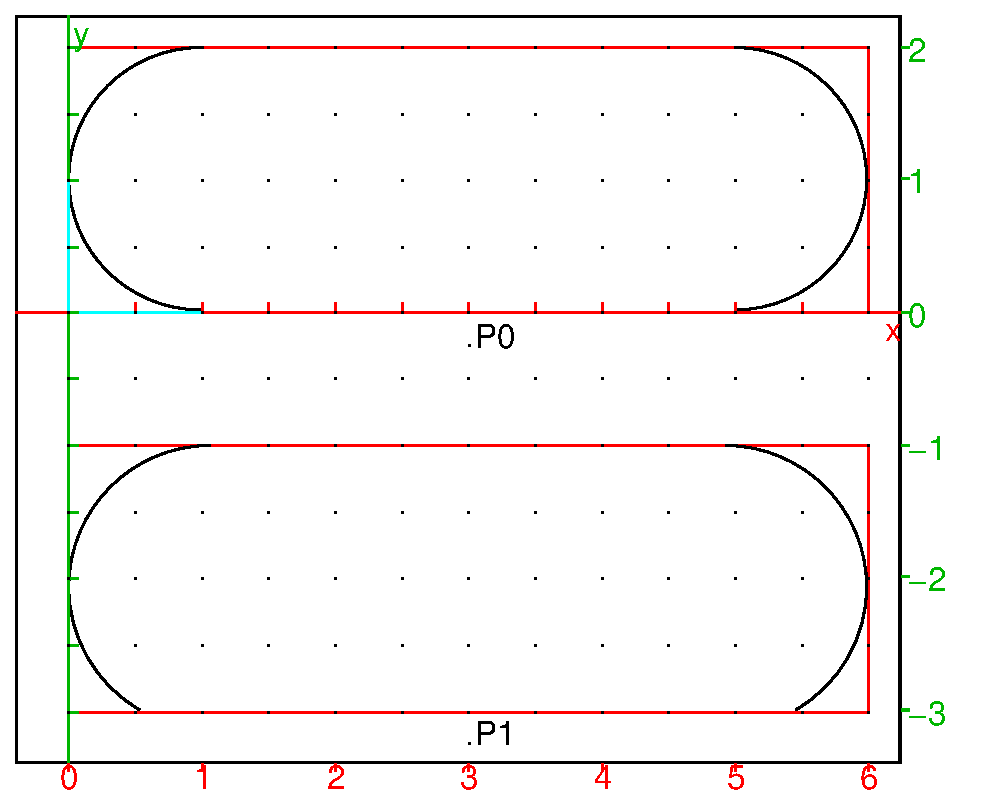
\includegraphics[width=\textwidth]{bassin01}\\
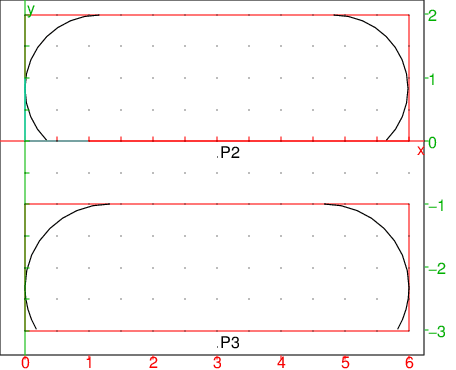
\includegraphics[width=\textwidth]{bassin23}\\
Dessiner ces 4 piscines avec {\tt Xcas} et calculer l'aire de ces 4 piscines.\\
Est-ce que l'aire de la plus grande piscine correspond \`a l'aire du plus 
grand bassin ? 

L'aire de la piscine $P_k$ est \'egale \`a la somme de l'aire du bassin $B_k$ 
et de l'aire du rectangle de largeur $a=2$ et de longueur $3a-2r_k=2(3-r_k)$.
On tape :\\
{\tt a:=2}\\
On tape :\\
{\tt evalf(A0+2*(6-2*r0))}\\
On obtient :\\
{\tt 11.1415926536}\\
On tape :\\
{\tt evalf(A1+4*(3-r1))}\\
On obtient :\\
{\tt 11.2176515906}\\
On tape :\\
{\tt evalf(A2+4*(3-r2))}\\
On obtient :\\
{\tt 11.2340725067}\\
On tape :\\
{\tt evalf(A3+4*(3-r3))}\\
On obtient :\\
{\tt 11.1598360965}\\
$P_2$ est la plus grande piscine et elle correspond \`a l'aire du bassin $B_2$.
En effet lorsque l'aire des bassins augmente, l'aire du rectangle int\'erieur
diminue...donc on ne peut rien dire \`a priori.
\end{document}
